% Tikz plot for UQ. This is based on the tikz code of
% Fabian Schuh for the tikz examples website
\documentclass[10pt,final,xcolor=dvipsnames]{beamer}
%\usepackage{etex}

\usetheme{Madrid}

\usepackage{xspace}
%\usepackage{enumitem}
\usepackage[mathscr]{euscript}
\usepackage{subfigure}
\hypersetup{colorlinks,linkcolor=,urlcolor=blue}

% \usetheme{Boadilla}
% \usecolortheme{seahorse}

% the macros, packages, etc:
\usepackage[absolute,overlay]{textpos}
\setbeamertemplate{items}[ball]
\setbeamertemplate{blocks}[rounded][shadow=true]
\setbeamertemplate{navigation symbols}{}
\newenvironment{reference}[2]{%
  \begin{textblock*}{\textwidth}(#1,#2)
  \scriptsize{\it\color{black}}}{\end{textblock*}}
\setbeamertemplate{blocks}[rounded]% [shadow=false]
\newenvironment{boxalertenv}{\begin{altenv}%
      {\usebeamertemplate{alerted text begin}\usebeamercolor[fg]{alerted text}\usebeamerfont{alerted text}\colorbox{bg}}
      {\usebeamertemplate{alerted text end}}{\color{.}}{}}{\end{altenv}}

\usepackage{graphicx}
\usepackage{multirow,color}
\usepackage{bbm}
\usepackage{amsfonts,amsmath,amssymb,amsbsy,amsthm}
\usepackage{movie15}
\definecolor{themec}{RGB}{51,108,121}

%\usepackage{movie15}
%\usepackage{multimedia}
% custom commands (add your own macros here)

\definecolor{bronze}{rgb}{0.8, 0.5, 0.2}
\definecolor{goldenyellow}{rgb}{1.0, 0.87, 0.0}
\definecolor{amber}{rgb}{1.0, 0.75, 0.0}
\definecolor{azure}{rgb}{0.94, 1.0, 1.0}
\definecolor{bittersweet}{rgb}{1.0, 0.44, 0.37}
\definecolor{brass}{rgb}{0.71, 0.65, 0.26}
\definecolor{camel}{rgb}{0.76, 0.6, 0.42}
\setbeamercolor{block body}{bg=camel!30}
\usefonttheme[onlymath]{serif}
\usepackage{color}

\usepackage{amsmath}
\usepackage{mathtools}
\usepackage{tikz}
\usepackage{amsfonts,amsmath,amssymb,amsbsy,amsthm}
%\usecolortheme{tango}

%\usefonttheme{serif}     % Font theme: serif
%\usefonttheme[stillsansseriftext]{serif} 
%\renewcommand*\familydefault{\sfdefault}

\usepackage{pgf}
%\usepackage{pgfplots}
\usepackage{amssymb}
\usepackage{amsmath}
\usepackage{tikz}
\usepackage{verbatim}
%\usepackage{movie15}
\usepackage{tikz,pgfplots}

%\usepackage[active,tightpage]{preview}
%\PreviewEnvironment{tikzpicture}
\usetikzlibrary{arrows,automata}
\usetikzlibrary{positioning}
\usetikzlibrary{fit}

%%%%%%%%%%%%%%%%%%%%%%%%%%%%%%%%%%%%%%%%%%%%%%%%%%%%%
%% this def file is based on the ccgodef
%%%%%%%%%%%%%%%%%%%%%%%%%%%%%%%%%%%%%%%%%%%%%%%%%%%%%
% packages
%\usepackage{booktabs}
%\usepackage[mathscr]{euscript}
%\usepackage{color}
%% mathdesgin or ams
%%\usepackage{amssymb,mathrsfs}
%\usepackage{graphicx}
%\usepackage{algorithmic,algorithm}
%\usepackage{tikz,pgfplots}
%\usepackage{upgreek}
%%\usepackage{showkeys,cite}
%\usepackage{multirow}
%\usepackage{yfonts}
%\usepackage{mathtools}
%\usepackage[normalem]{ulem}
%\usepackage{latexsym}
%\usepackage{url}
%\usepackage{amsmath,amssymb,amsbsy,amsfonts}
%\usepackage{enumitem}

\newcommand{\zapspace}{\topsep=0pt\partopsep=0pt\itemsep=0pt\parskip=0pt}

%% Notice macros
%\newcommand{\notice}[1]{\textcolor{Chameleon3}{#1}}
%\newcommand{\Notice}[1]{\textcolor{ScarletRed2}{#1}}
%\newcommand{\nnote}[1]{\noindent\emph{\textcolor{grass}{N: #1\,}}}
%\newcommand{\unote}[1]{\noindent\emph{\textcolor{blue}{U: #1\,}}}
%\newcommand{\onote}[1]{\noindent\emph{\textcolor{red}{O: #1\,}}}
%
%% colors
%\definecolor{utorange}{rgb}{0.8,0.33,0.}
%\definecolor{themec}{RGB}{51,108,121}
%\definecolor{darkred}{rgb}{.6,.1,.1}
%\definecolor{darkblue}{rgb}{.1,.1,.9}
%\definecolor{greenback}{rgb}{.19,.94,.13}
%\definecolor{orange}{rgb}{.76,.39,.13}
%\definecolor{grass}{rgb}{.19,.64,.13}
%\definecolor{sierp}{RGB}{209,28,209}
%\definecolor{bgorange}{rgb}{1.,.95,.78}
%\definecolor{grassgreen}{RGB}{92,135,39}
%\definecolor{thinbox}{rgb}{.7,.8,1.}

% general
\newcommand{\defeq}{\vcentcolon=}
%\newcommand{\del}[2]{\frac{\partial{#1}}{\partial{#2}}}
\renewcommand{\vec}[1]{{\mathchoice
                     {\mbox{\boldmath$\displaystyle{#1}$}}
                     {\mbox{\boldmath$\textstyle{#1}$}}
                     {\mbox{\boldmath$\scriptstyle{#1}$}}
                     {\mbox{\boldmath$\scriptscriptstyle{#1}$}}}}
\renewcommand{\ker}{\mathsf{ker}}
\newcommand{\ran}{\mathsf{range}}
\newcommand{\dom}{\mathsf{dom}}
\newcommand{\trace}{\mathsf{tr}}
\newcommand{\eps}{\varepsilon}
%\newcommand{\norm}[1]{\left\| {#1} \right\|}
\newcommand{\ip}[2]{{\left\langle {#1}, {#2} \right\rangle}}
\newcommand{\mip}[2]{\left\langle{#1}, {#2}\right\rangle_{\!\scriptscriptstyle{\text{M}}}}
\newcommand{\mat}[1]{\mathbf{{#1}}}
\newcommand\restr[2]{{
  \left.\kern-\nulldelimiterspace % automatically resize the bar with \right
  {#1}\vphantom{\big|} \right|_{#2}}}
\newcommand{\angles}[1]{\left\langle #1 \right\rangle}

% sets of numbers
\newcommand{\R}{\mathbb{R}}
\newcommand{\Z}{\mathbb{Z}}
\newcommand{\N}{\mathbb{N}}

\newcommand{\BB}{\mat{B}}
\newcommand{\Amat}{\mat{A}}
\newcommand{\VV}{\mat{V}}
\newcommand{\RR}{\mat{R}}

% commonly used mathcals
\newcommand{\A}{\mathcal{A}}
\newcommand{\B}{\mathcal{B}}
\newcommand{\C}{\mathcal{C}}
\newcommand{\D}{\mathcal{D}}
\newcommand{\E}{\mathcal{E}}
\newcommand{\F}{\mathcal{F}}
\newcommand{\G}{\mathcal{G}}
\newcommand{\J}{\mathcal{J}}
\newcommand{\U}{\mathcal{U}}
\newcommand{\Reg}{\mathcal{R}}

% shorthands
\newcommand{\bit}{\begin{itemize}}
\newcommand{\eit}{\end{itemize}}
\newcommand{\bdm} {\begin{displaymath}}
\newcommand{\edm} {\end{displaymath}}

% Probability (general)
\newcommand{\prob}{\mathsf{Prob}}
\newcommand{\borel}{\mathscr{B}}
\newcommand{\ave}{\mathsf{E}}
\newcommand{\GM}[2]{\mathcal{N}\!\left( {#1}, {#2}\right)}

% Bayesian stuff

\newcommand{\noisem}{\mu_{\text{noise}}}
\newcommand{\obs}{\vec{d}}
\newcommand{\ipar}{m}

\newcommand{\iparpr}{m_{\text{pr}}}
\newcommand{\iparref}{m_{\text{ref}}}
\newcommand{\iparmap}{m_{\scriptscriptstyle\text{MAP}}}
\newcommand{\dpar}{\vec{m}}
\newcommand{\dparmap}{\vec{m}_{\scriptscriptstyle\text{MAP}}}
%\newcommand{\priorm}{\mu_{\text{pr}}}
%\newcommand{\postm}{\mu_{\text{post}}}
\newcommand{\M}{\mat{M}}% the Mass matrix
%\newcommand{\ff}{\vec{f}}     % parameter-to-obs MAP
\newcommand{\ff}{\mathcal{F}} % parameter-to-obs MAP
\newcommand{\aff}{\tilde{\mathcal{F}}} % parameter-to-obs MAP
\newcommand{\noise}{\bs e}
\newcommand{\observables}{\bs d}
\newcommand{\data}{ \observables_{\rm{obs}} }
\newcommand{\uobs}{ \uu_{\rm{obs}} }
\newcommand{\datacomponent}[1]{ \observables_{\rm{obs}}^{#1} }
\newcommand{\FF}{{\ensuremath{\mat{F}}}}
\newcommand{\W}{{\ensuremath{\mat{W}}}}
\newcommand{\I}{{\ensuremath{\mat{I}}}}

\newcommand{\prior} {\pi_{\mbox{\tiny prior}}}
\newcommand{\like}{\pi_{\mbox{\tiny like}}}
\newcommand{\piobs}{\pi_{\mbox{\tiny obs}}}
\newcommand{\post}{\pi_{\mbox{\tiny post}}}
\newcommand{\pinoise}{\pi_{\mbox{\tiny noise}}}

\newcommand{\mupost}{\mu_{\mbox{\tiny post}}}
\newcommand{\muprior}{\mu_{\mbox{\tiny prior}}}

\newcommand{\ncov} {\bs{\Gamma}_{\!\mbox{\tiny noise}} }
\newcommand{\prcov} {\bs{\Gamma}_{\!\mbox{\tiny prior}} }
\newcommand{\postcov} {\bs{\Gamma}_{\!\mbox{\tiny post}} }
\newcommand{\aFF}{{\tilde{\ensuremath{\mat{F}}}}}
\newcommand{\ncovw} {\bs{W}}
\newcommand{\prcovr} {\bs{R}}

\newcommand{\Cprior}{\mathcal{C}_{\text{\tiny{prior}}}}
\newcommand{\Cpost}{\mathcal{C}_{\text{\tiny{post}}}}

\newcommand{\map} {{m}_{\mbox{\tiny MAP}} }
\newcommand{\dmap} {{\vec{m}}_{\mbox{\tiny MAP}} }
\newcommand{\mpr} {{\vec{m}}_{\mbox{\tiny pr}} }
\newcommand{\dbeta}{\vec{\beta}}
\newcommand{\dn}{\vec{n}}



\newcommand{\Hpost}  { \bs H }
\newcommand{\Hmisfit}{ \mat{H}_{\mbox{\tiny misfit}} }
\newcommand{\tHmisfit}{\tilde{\mat{H}}_{\mbox{\tiny misfit}} }
\newcommand{\HT}{\matrix{\tilde{H}}_{\mbox{\tiny misfit}}}
\newcommand{\HTinf}{\tilde{H}_{\text{misfit}}}
\newcommand{\Vr} {\bs V_r}
\newcommand{\Dr} {\bs D_r}
\newcommand{\Ir} {\bs I_r}

%\newcommand{\Ge}{ \ensuremath{\matrix{G}}_{\!\mbox{\tiny e}}}
%\newcommand{\Op}{ \ensuremath{\matrix{O}}_{\!\mbox{\tiny p}}}
\newcommand{\Ge}{ \mathcal{G}_{\!\mbox{\tiny e}}}
\newcommand{\Op}{ \mathcal{O}_{\!\mbox{\tiny p}}}
\newcommand{\HH}{ \ensuremath{\matrix{H}} }
\newcommand{\SI}{ \ensuremath{{\Sigma}} }
\newcommand{\PP}{ \ensuremath{\matrix{\Psi}} }
%\newcommand{\WW}{ \ensuremath{\matrix{W}} }
\newcommand{\WW}{ \mathcal{W}}

% Macros for three different forms of adjoint operator
\newcommand{\adjMacroMM}[1]{{#1}^*}
\newcommand{\adjMacroME}[1]{{#1}^\natural}
\newcommand{\adjMacroEM}[1]{{#1}^\diamond}
\newcommand{\adjMacroEMINV}[1]{{#1}^{-\diamond}}
\newcommand{\Aadj}{\adjMacroMM{\A}}
\newcommand{\Badj}{\adjMacroMM{\BB}}
\newcommand{\iFadj}{\adjMacroME{\iF}}
\newcommand{\Fadj}{\adjMacroME{\F}}
\newcommand{\Vadj}{\adjMacroEM{\VV}}
\newcommand{\Ladj}{\adjMacroEM{\L}}

\def\bfG{\mbox{\boldmath$G$}}
\newcommand{\mc}[1]{\mathcal{#1}}

%%%%%%%%%%%%%%%%%%%%%%%%%%%%%%%%%%%%
% custom commands to the sc14 paper
%%%%%%%%%%%%%%%%%%%%%%%%%%%%%%%%%%%%
\newcommand{\SNR}{\ensuremath{\text{SNR}}}

\newcommand{\gbf}[1]{\boldsymbol{#1}}
\newcommand{\bs}[1]{\ensuremath{\boldsymbol{#1}}}

\newcommand{\edot}{\dot{\gbf{\varepsilon}}}
\newcommand{\edotsec}{\edot_\mathrm{II}}
\newcommand{\secinve}{\edot_\mathrm{II}}

\DeclareMathOperator{\sym}{sym}
%\DeclareMathOperator{\trace}{tr}
%\DeclareMathOperator{\diag}{diag}

\newcommand{\Div}{\mbox{div}}
\newcommand{\Grad}{{\bf \nabla}}
\newcommand{\grad}{\nabla}

\newcommand{\pt}{\tilde{p}}
\newcommand{\vt}{\tilde{\vv}}
\newcommand{\qt}{\tilde{q}}
\newcommand{\betat}{\tilde{\beta}}

\newcommand{\uh}{\hat{\uu}}
\newcommand{\ph}{\hat{p}}
\newcommand{\vh}{\hat{\vv}}
\newcommand{\qh}{\hat{q}}
\newcommand{\betah}{\hat{\beta}}

\renewcommand{\vec}[1]{\gbf{#1}}
\newcommand{\cvec}[1]{{#1}}

\newcommand{\uu}{\ensuremath{\vec{u}}}
\newcommand{\vv}{\ensuremath{\vec{v}}}

\definecolor{darkblue}{rgb}{.1,.1,.9}
\definecolor{utorange}{rgb}{0.8,0.33,0.}
% this are only needed for presentations
\newcommand{\tcb}[1]{\textcolor{blue}{{#1}}}
\newcommand{\tcdb}[1]{\textcolor{utorange}{{#1}}}
\newcommand{\tcr}[1]{\ensuremath{\textcolor{red}{{#1}}}}
\newcommand{\tcdr}[1]{\textcolor{darkred}{{#1}}}
\newcommand{\tcm}[1]{\textcolor{ForestGreen}{{#1}}}
\newcommand{\tcmag}[1]{\textcolor{magenta}{{#1}}}
\newcommand{\tco}[1]{\textcolor{VioletRed}{{#1}}}
\newcommand{\tcc}[1]{\textcolor{cyan}{{#1}}}
\newcommand{\dg}[1]{\textcolor{black!65!green}{{#1}}}
\newcommand{\tcg}[1]{\textcolor{blue!70!black!30!green}{{#1}}}
\newcommand{\tcdg}[1]{\textcolor{blue!20!black!50!green}{{#1}}}
\newcommand{\tcch}[1]{\textcolor{cyan}{\hat{{#1}}}}
\newcommand{\tcmhb}[1]{\textcolor{magenta}{\hat{\gbf{{#1}}}}}
\newcommand{\tcmh}[1]{\textcolor{magenta}{\hat{{#1}}}}
\newcommand{\tcbb}[1]{\textcolor{blue}{\gbf{{#1}}}}
\newcommand{\tcgb}[1]{\textcolor{grass}{\gbf{{#1}}}}
\newcommand{\tcct}[1]{\textcolor{cyan}{\tilde{{#1}}}}
\newcommand{\tcmtb}[1]{\textcolor{magenta}{\tilde{\gbf{{#1}}}}}
\newcommand{\tcmt}[1]{\textcolor{magenta}{\tilde{{#1}}}}
\newcommand{\tcotb}[1]{\textcolor{utorange}{\tilde{\gbf{{#1}}}}}
\newcommand{\tcot}[1]{\textcolor{utorange}{\tilde{{#1}}}}
\newcommand{\tcohb}[1]{\textcolor{utorange}{\hat{\gbf{{#1}}}}}
\newcommand{\tcoh}[1]{\textcolor{utorange}{\hat{{#1}}}}

\renewcommand{\matrix}[1] {\ensuremath{\boldsymbol{#1}}}

\newcommand{\bndFS}{\Gamma_{\!\mbox{\scriptsize $FS$}}}
\newcommand{\bndB}{\Gamma_{\!\mbox{\scriptsize $B$}}}
\newcommand{\bndT}{\Gamma_{\!\mbox{\scriptsize $T$}}}

\usepackage{xspace}
\newcommand{\software}[1]{\texttt{#1}\xspace}
\newcommand{\hip}{\texttt{hIPPYlib}\xspace}
\newcommand{\bhip}{\texttt{{\bf hIPPYlib}}\xspace}
\newcommand{\Fe}{\texttt{FEniCS}\xspace}
\newcommand{\pet}{\texttt{PETSc}\xspace}


\newcommand{\del}{\partial}
%\newcommand{\D}{\mathcal{D}}
\newcommand{\Ns}{{N_s}}
\newcommand{\Ntau}{{N_{\tau}}}
\newcommand{\iFF}{\mathcal{F}}
%\newcommand{\priorm}{\muprior}
\newcommand{\Acal}{\mc{A}}
%\newcommand{\postm}{\mupost}
\newcommand{\iparpost}{\ipar_\text{post}}
\newcommand{\dd}{\vec{\bar{d}}}
\newcommand{\obsop}{\mathcal{B}}

\newcommand{\GN}{\ensuremath{\Gamma_{\!\!N}}}
\newcommand{\Exp}[1]{e^{{#1}}}
\newcommand{\GD}{\ensuremath{\Gamma_{\!\!D}}}
\newcommand{\Vg}{\mathscr{V}_{\!g}}
\newcommand{\V}{\mathscr{V}_{\!\scriptscriptstyle{0}}}
\newcommand{\eip}[2]{\left\langle{#1}, {#2}\right\rangle_{\!{\R^q}}}
\newcommand{\Wn}{\mat{W}_{\!\sigma}}
\newcommand{\cip}[2]{\left\langle{#1}, {#2}\right\rangle_{\!\CM}}
\newcommand{\CM}{\mathscr{E}}
\newcommand{\LI}{\mathscr{L}}
\renewcommand{\H}{\mathcal{H}}
\newcommand{\Nd}{{n_{\text{d}}}}
\newcommand{\Ntr}{{n_{\text{tr}}}}
\newcommand{\ipart}{m_{\scriptscriptstyle\text{true}}}
\newcommand{\ut}[1]{\ensuremath{\tilde{#1}}}

\newcommand{\LRp}[1]{\left( #1 \right)}
\newcommand{\LRs}[1]{\left[ #1 \right]}
\newcommand{\LRa}[1]{\left< #1 \right>}
\newcommand{\LRc}[1]{\left\{ #1 \right\}}

\newcommand{\xx}{\ensuremath{\boldsymbol x}}
\newcommand{\rr}{\ensuremath{\boldsymbol r}}
\newcommand{\e}{\ensuremath{\boldsymbol e}}
\newcommand{\x}{\xx}
\newcommand{\y}{\ensuremath{\boldsymbol y}}
\newcommand{\z}{\ensuremath{\boldsymbol z}}
\renewcommand{\r}{\ensuremath{\boldsymbol r}}
\newcommand{\s}{\ensuremath{\boldsymbol s}}

\newcommand{\hilb}{\mathscr{H}}
\newcommand{\half} {\ensuremath{\frac{1}{2}}}
\newcommand{\nor}[1]{\left\| #1 \right\|}
\newcommand{\equaldef}{{:=}}
\newcommand{\iFFadj}{\adjMacroMM{\iFF}}

\newcommand{\istate}{u}
\newcommand{\iparspace}{\mathcal{M}}
\newcommand{\iadj}{p}
\DeclareMathOperator*{\argmin}{argmin} 
\DeclareMathOperator{\diag}{diag} 


\newcommand{\err}{\vec{\eta}}
\newcommand{\beps}{\bs{\eps}}
\newcommand{\bbeps}{\bar{\bs{\eps}}}
\newcommand{\bnu}{\bs{\nu}}
\newcommand{\ncovbeps} {\bs{\Gamma}_{\!\mbox{\tiny \beps}} }
\newcommand{\ncovbnu} {\bs{\Gamma}_{\!\mbox{\tiny \bnu}} }
\newcommand{\norm}[2][]{\left\Vert #2\right\Vert_{#1}}
\newcommand{\dbetamap}{\vec{\beta}_{\scriptscriptstyle\text{MAP}}}
\newcommand{\betamap}{{\beta}_{\scriptscriptstyle\text{MAP}}}
\newcommand{\smallB}{\scriptscriptstyle\text{B}}
\definecolor{lightblue}{cmyk}{0.88,0.44,0,0.07}
\newcommand{\betapr}{\beta_{\text{pr}}}
\newcommand{\ntrue}{a_{\scriptscriptstyle\text{true}}}
\newcommand{\NoiseForcing}{\xi}
\newcommand{\ProbMeasClass}{\mathcal{P}}
\newcommand{\ProbMeas}{\mathbbm{P}}
\newcommand{\SigmaAlg}{F}

\newcommand{\Hmatrix}{\bs{H}}

\newcommand{\iparb}{\bar{\ipar}}
\newcommand{\euclidnorm}[1]{\left\| {#1} \right\|_2}
\newcommand{\incu}{\upupsilon}
\newcommand{\incp}{\uprho}
\newcommand{\QoIquad}{\QoI_\text{quad}}
\newcommand{\tcblue}[1]{\textcolor{blue}{#1}}
\newcommand{\betad}{\bs{\beta}}

\newcommand{\preconditioner}{\widetilde{H}}
\newcommand{\impulseresponse}{\phi}
\newcommand{\spatialmean}{\mu}
\newcommand{\Aop}{\mathcal{A}}

\tikzset{
    state/.style={
           rectangle,
           rounded corners,
           draw=black, very thick,
           minimum height=3em,
           inner sep=1pt,
           text centered,
           },
}

\newcommand{\Aker}{\Phi}
%\DeclareMathOperator{\diag}{diag}
%\newcommand{\Hmatrix}{\bs{H}}
\newcommand{\Hm}{\mathcal{H}}

% argument #1: any options
\newenvironment{customlegend}[1][]{%
    \begingroup
    % inits/clears the lists (which might be populated from previous
    % axes):
    \csname pgfplots@init@cleared@structures\endcsname
    \pgfplotsset{#1}%
}{%
    % draws the legend:
    \csname pgfplots@createlegend\endcsname
    \endgroup
}
\def\addlegendimage{\csname pgfplots@addlegendimage\endcsname}

% title, authors, etc:
\title[Bayesian ice sheet inverse
  problems]{Exploiting Low-Dimensional Structure in Bayesian Inverse
  Problems Governed by Ice Sheet Flow Models\thanks{Research supported
    partially by NSF-DMS-CAREER-1654311 and NSF-OAC-1550547.}}
%\author[{Noemi
%    Petra}]{No\'{e}mi~Petra\inst{1}}

\author[Noemi Petra]{{No\'{e}mi~Petra},\inst{1}\\[2ex]
  {\small \textcolor{themec}{Joint work with:}}
  \\
  {\small Nick Alger},\inst{2}
  {\small Tucker Hartland},\inst{3}
  {\small Omar Ghattas}\inst{2}
}

\institute[UC Merced]{%
  {Department of Applied Mathematics, University of California, Merced}\\\smallskip
  \inst{2}{Oden Institute for Computational Engineering and Sciences, The University of Texas at Austin}\\\smallskip
  \inst{3}{Center for Applied Scientific Computing (CASC), Lawrence Livermore National Laboratory}
}

\date[February 27, 2024]
     {\footnotesize SIAM Conference on Uncertainty Quantification (UQ24) \\
       Tuesday, February 27}

 \begin{document}

 % -------------------------------------------------------------------
%%\AtBeginSubsection[]  % "Beamer, do the following at the start of every section"
%\AtBeginSection[]  % "Beamer, do the following at the start of every section"
%{
%  \begin{frame}<beamer>
%    \frametitle{Outline} % make a frame titled "Outline"
%    \small
%  %\tableofcontents[currentsubsection]  % show TOC and highlight current section
%  \tableofcontents[currentsection]  % show TOC and highlight current section
%\end{frame}
%}
%----------- titlepage ----------------------------------------------%
\begin{frame}[plain]
  \titlepage
\end{frame}
%% ----------------------------------------------------------------------------
%\begin{frame}
%  \frametitle{Acknowledgements}
%
%  {\bf Various parts of this research is joint work with:}
%  \vspace{0.02in}
%  \begin{itemize}
%  \item Omar Ghattas (UT Austin)
%  \item Toby Isaac (Georgia Tech)
%  \item Georg Stadler (NYU)
%  \item Umberto Villa (Washington University, St. Louis)
%  \item Hongyu (Alice) Zhu (United Technologies)
%  \end{itemize}
%
%  \begin{itemize}
%  \item Olalekan (Lekan) Babaniyi (Rochester Institute of Technology)
%  \item Tucker Hartland and Radoslav Vuchkov (UC Merced) 
%  \item Ruanui (Ru) Nicholson (University of Auckland)
%  \end{itemize}
%
%  \vspace{0.05in}
%  {\bf Funding:}
%  \vspace{0.02in}
%  \begin{itemize}
%  \item Partial funding for this research was provided by the
%    U.S. National Science Foundation, Software Infrastructure for
%    Sustained Innovation (SI2: SSE \& SSI) Program under grants
%    ACI-1550593, and ACI-1550547 and by the NSF Division of
%    Mathematical Sciences under the CAREER grant 1654311.
%  \end{itemize}
%\end{frame}
%% ----------------------------------------------------------------------------
\begin{frame}
  \frametitle{Outline}


  \begin{itemize}
  \item Motivation
    \vspace{0.02in}
    \begin{itemize}
    \item Why we need predictive models with quantified uncertainties
      to accurately anticipate future sea level rise?
      \vspace{0.02in}
    \item Why we need more efficient approximations of high rank
      Hessians?
    \end{itemize}
    \vspace{0.02in}
  \item Bayesian inverse problems governed by PDEs (preliminaries)
    \vspace{0.02in}
  \item Exploiting low-dimensional structure in Bayesian inverse problems governed by PDEs
    \vspace{0.02in}
    \begin{itemize}
    \item (Global) low rank approximation
      \vspace{0.02in}
    \item Hierarchical off-diagonal low rank (HODLR) approximation
      \vspace{0.02in}
    \item Point spread function approximation combined with
      hierarchical matrix (H-matrix) approximation
    \end{itemize}
    \vspace{0.02in}
  \item Example: Inversion for the basal friction
    coefficient in an ice sheet flow problem
    \vspace{0.02in}
  \item Conclusions
  \end{itemize}

\end{frame}
%-------------------------------------------------------------------
\begin{frame}
  \frametitle{Need predictive models with quantified uncertainties to accurately anticipate future sea
   level rise.}
\framesubtitle{Sea level projections from the IPCC 6th Assessment Report, 2021}
 \vspace{0.2in}
  \begin{columns}
    \begin{column}{0.7\paperwidth}
       \centering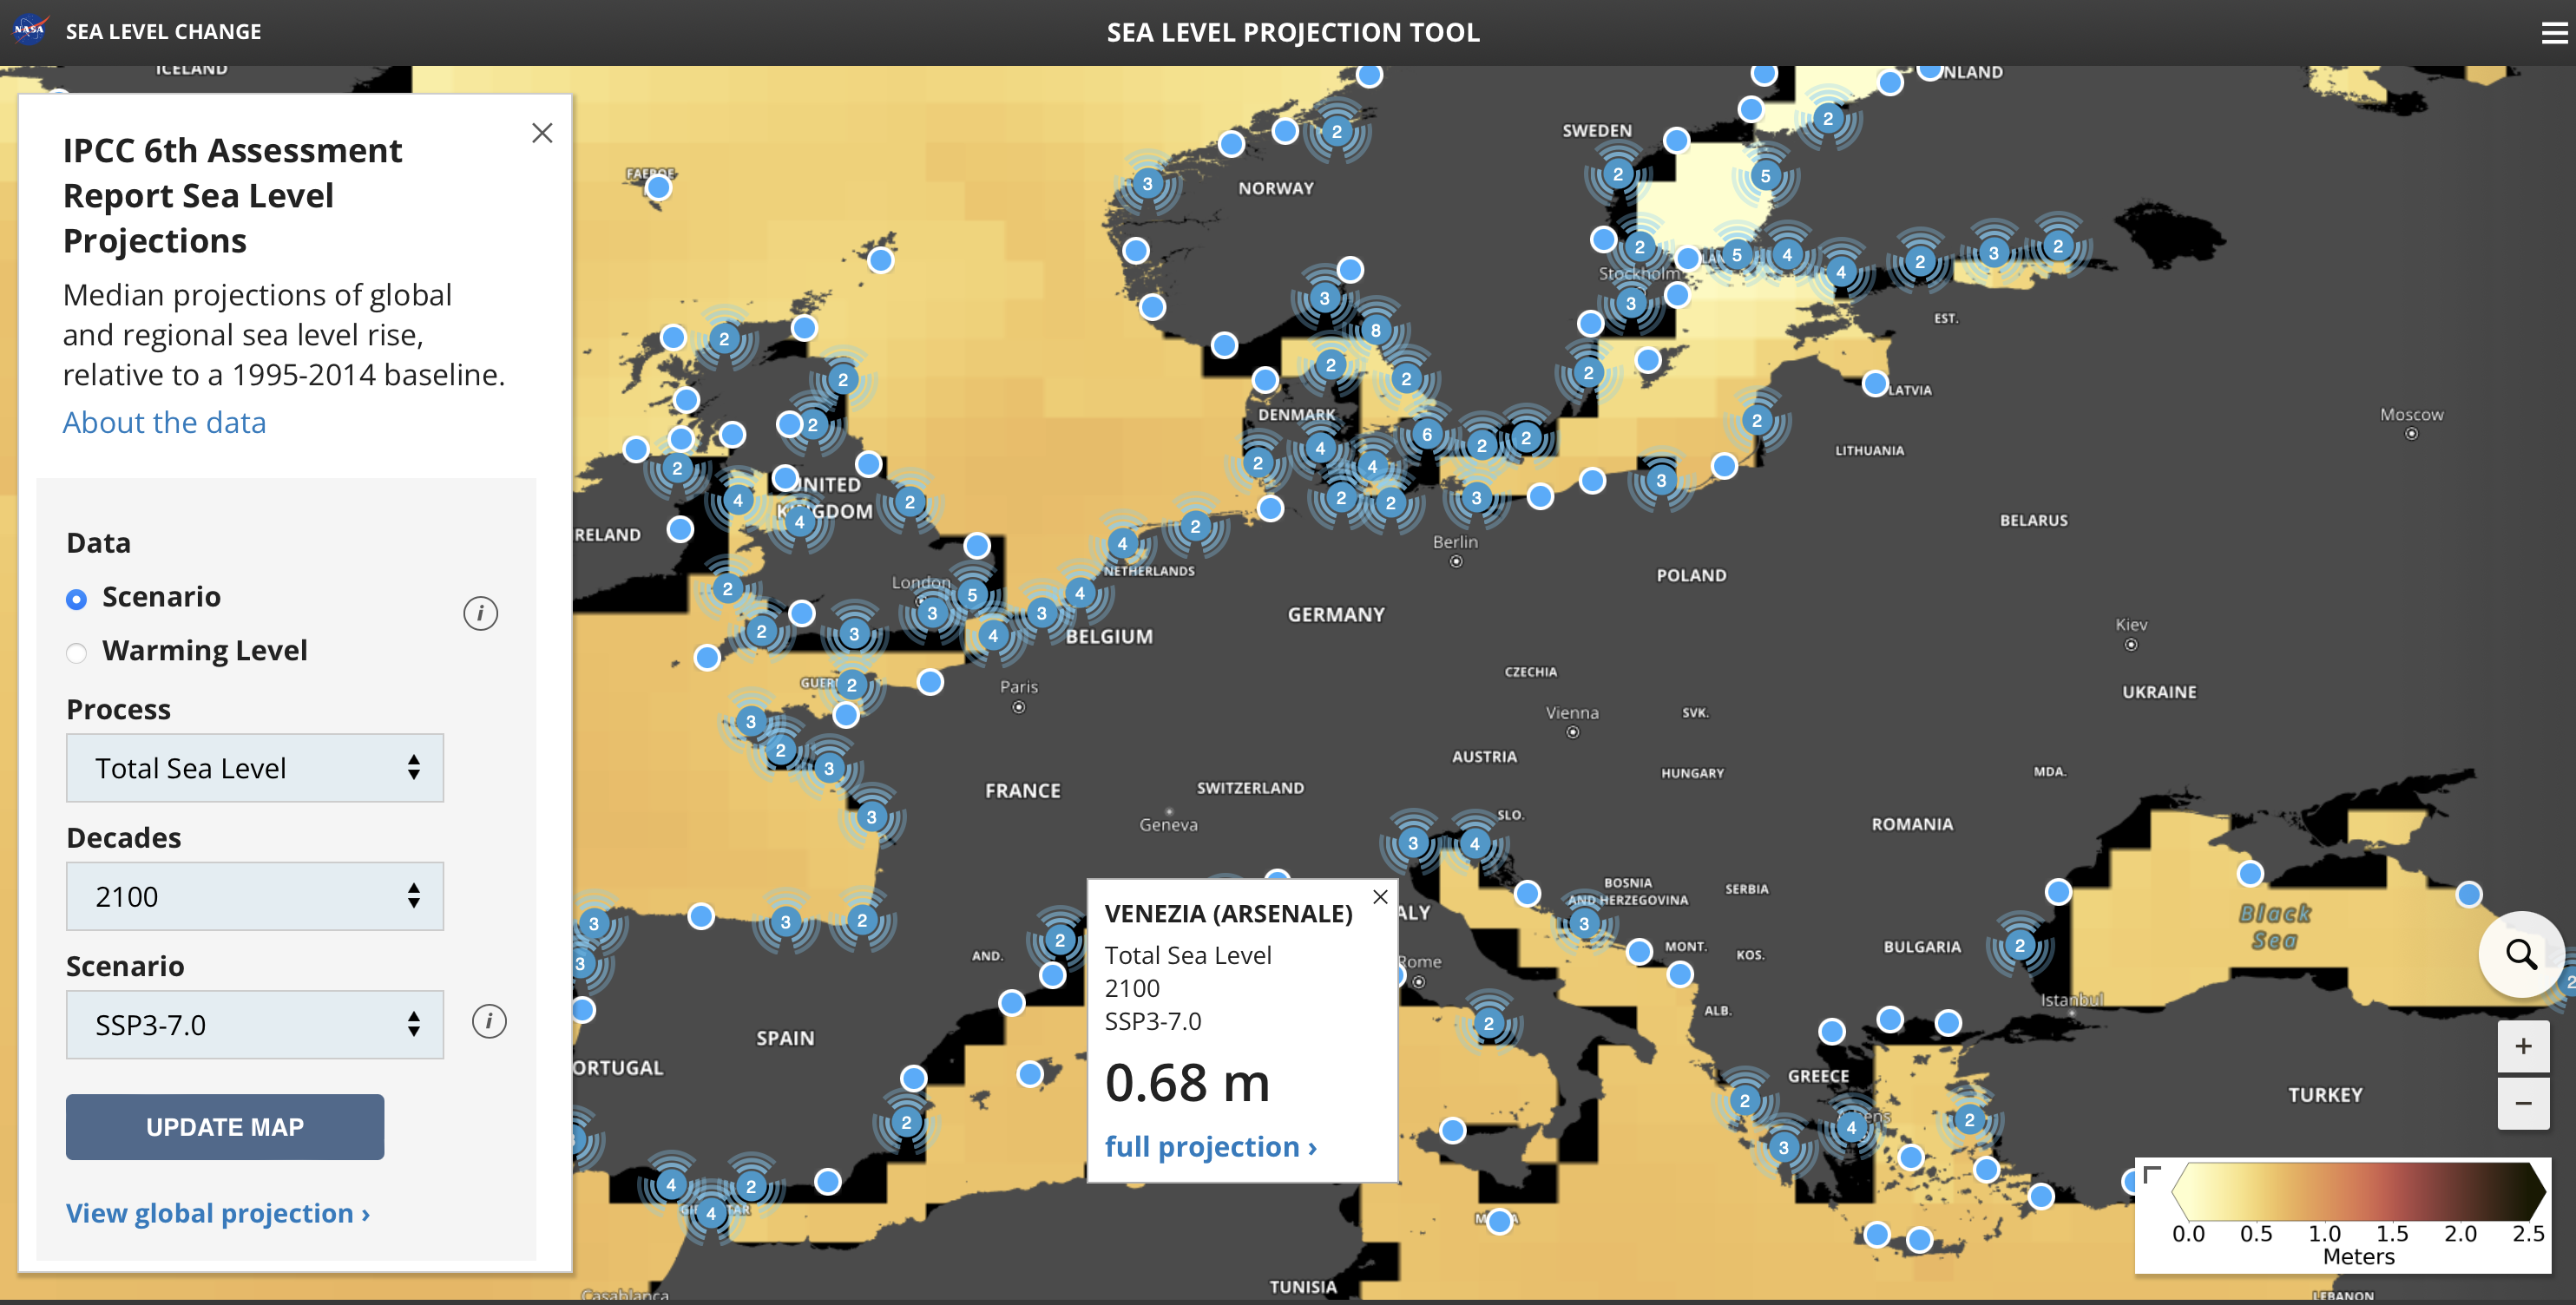
\includegraphics[width=0.85\columnwidth]{extraplots/venezia}
    \end{column}
    \hspace{-0.4in}
    \begin{column}{0.3\paperwidth}
    \vspace{0.1in}
      \centering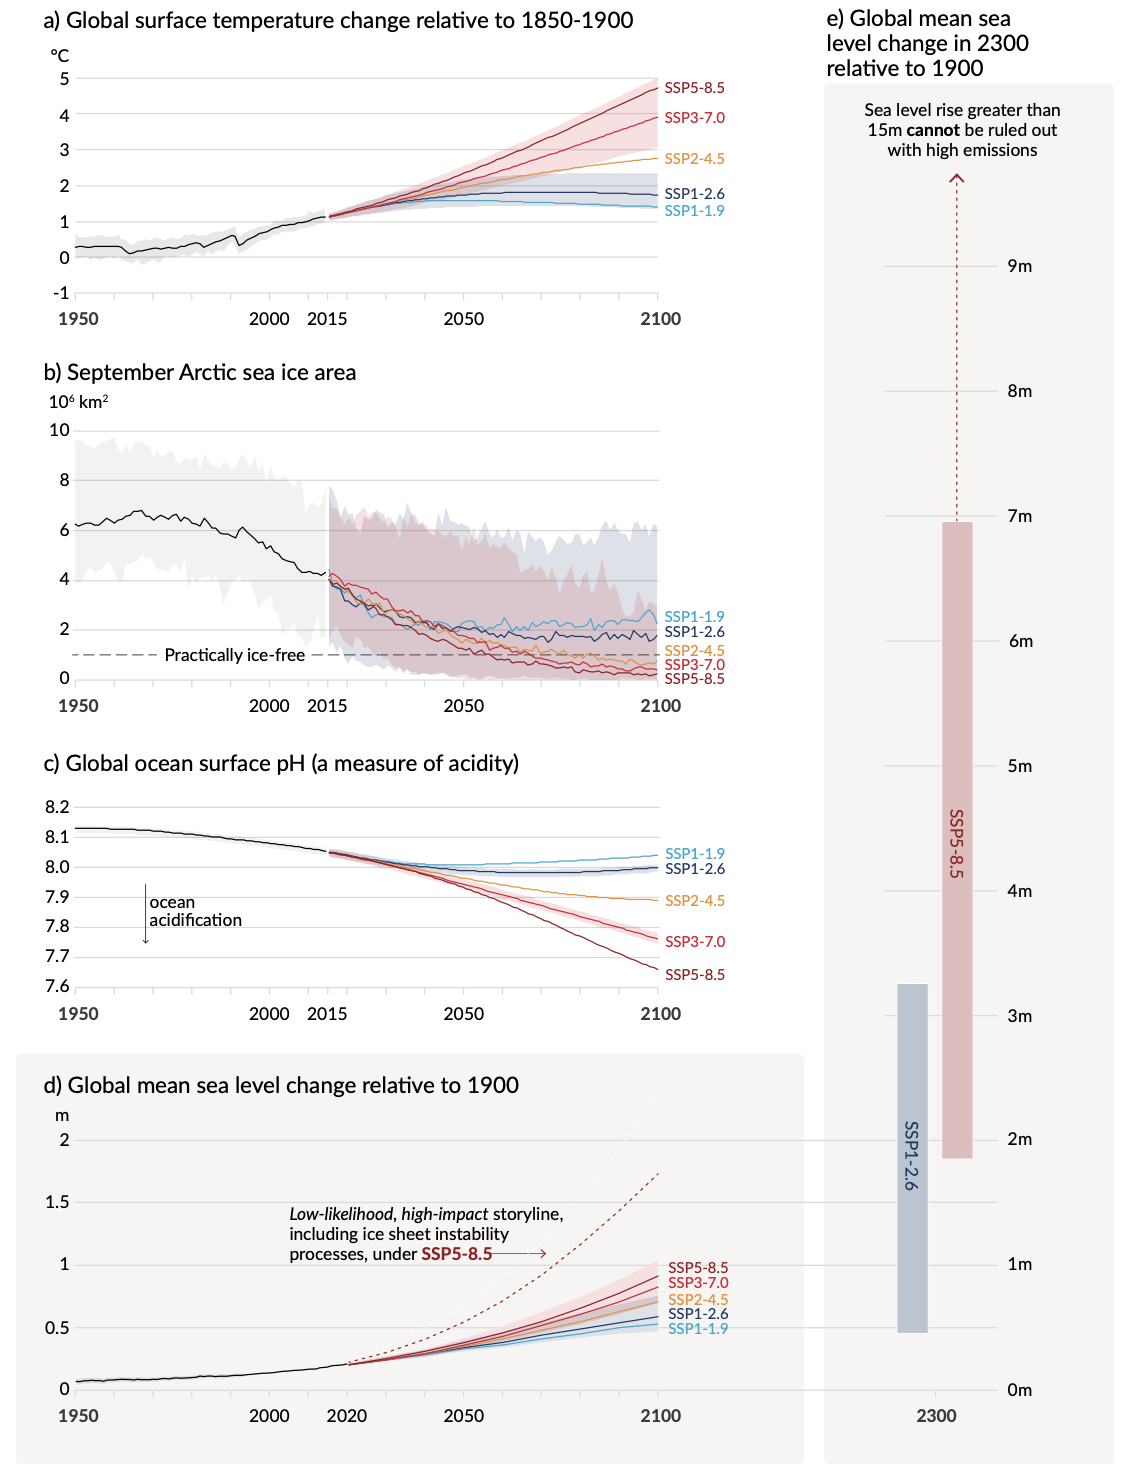
\includegraphics[width=0.85\columnwidth]{extraplots/ipcc-ar6-wgi-2021.png}
    \end{column}
  \end{columns}

  %\centering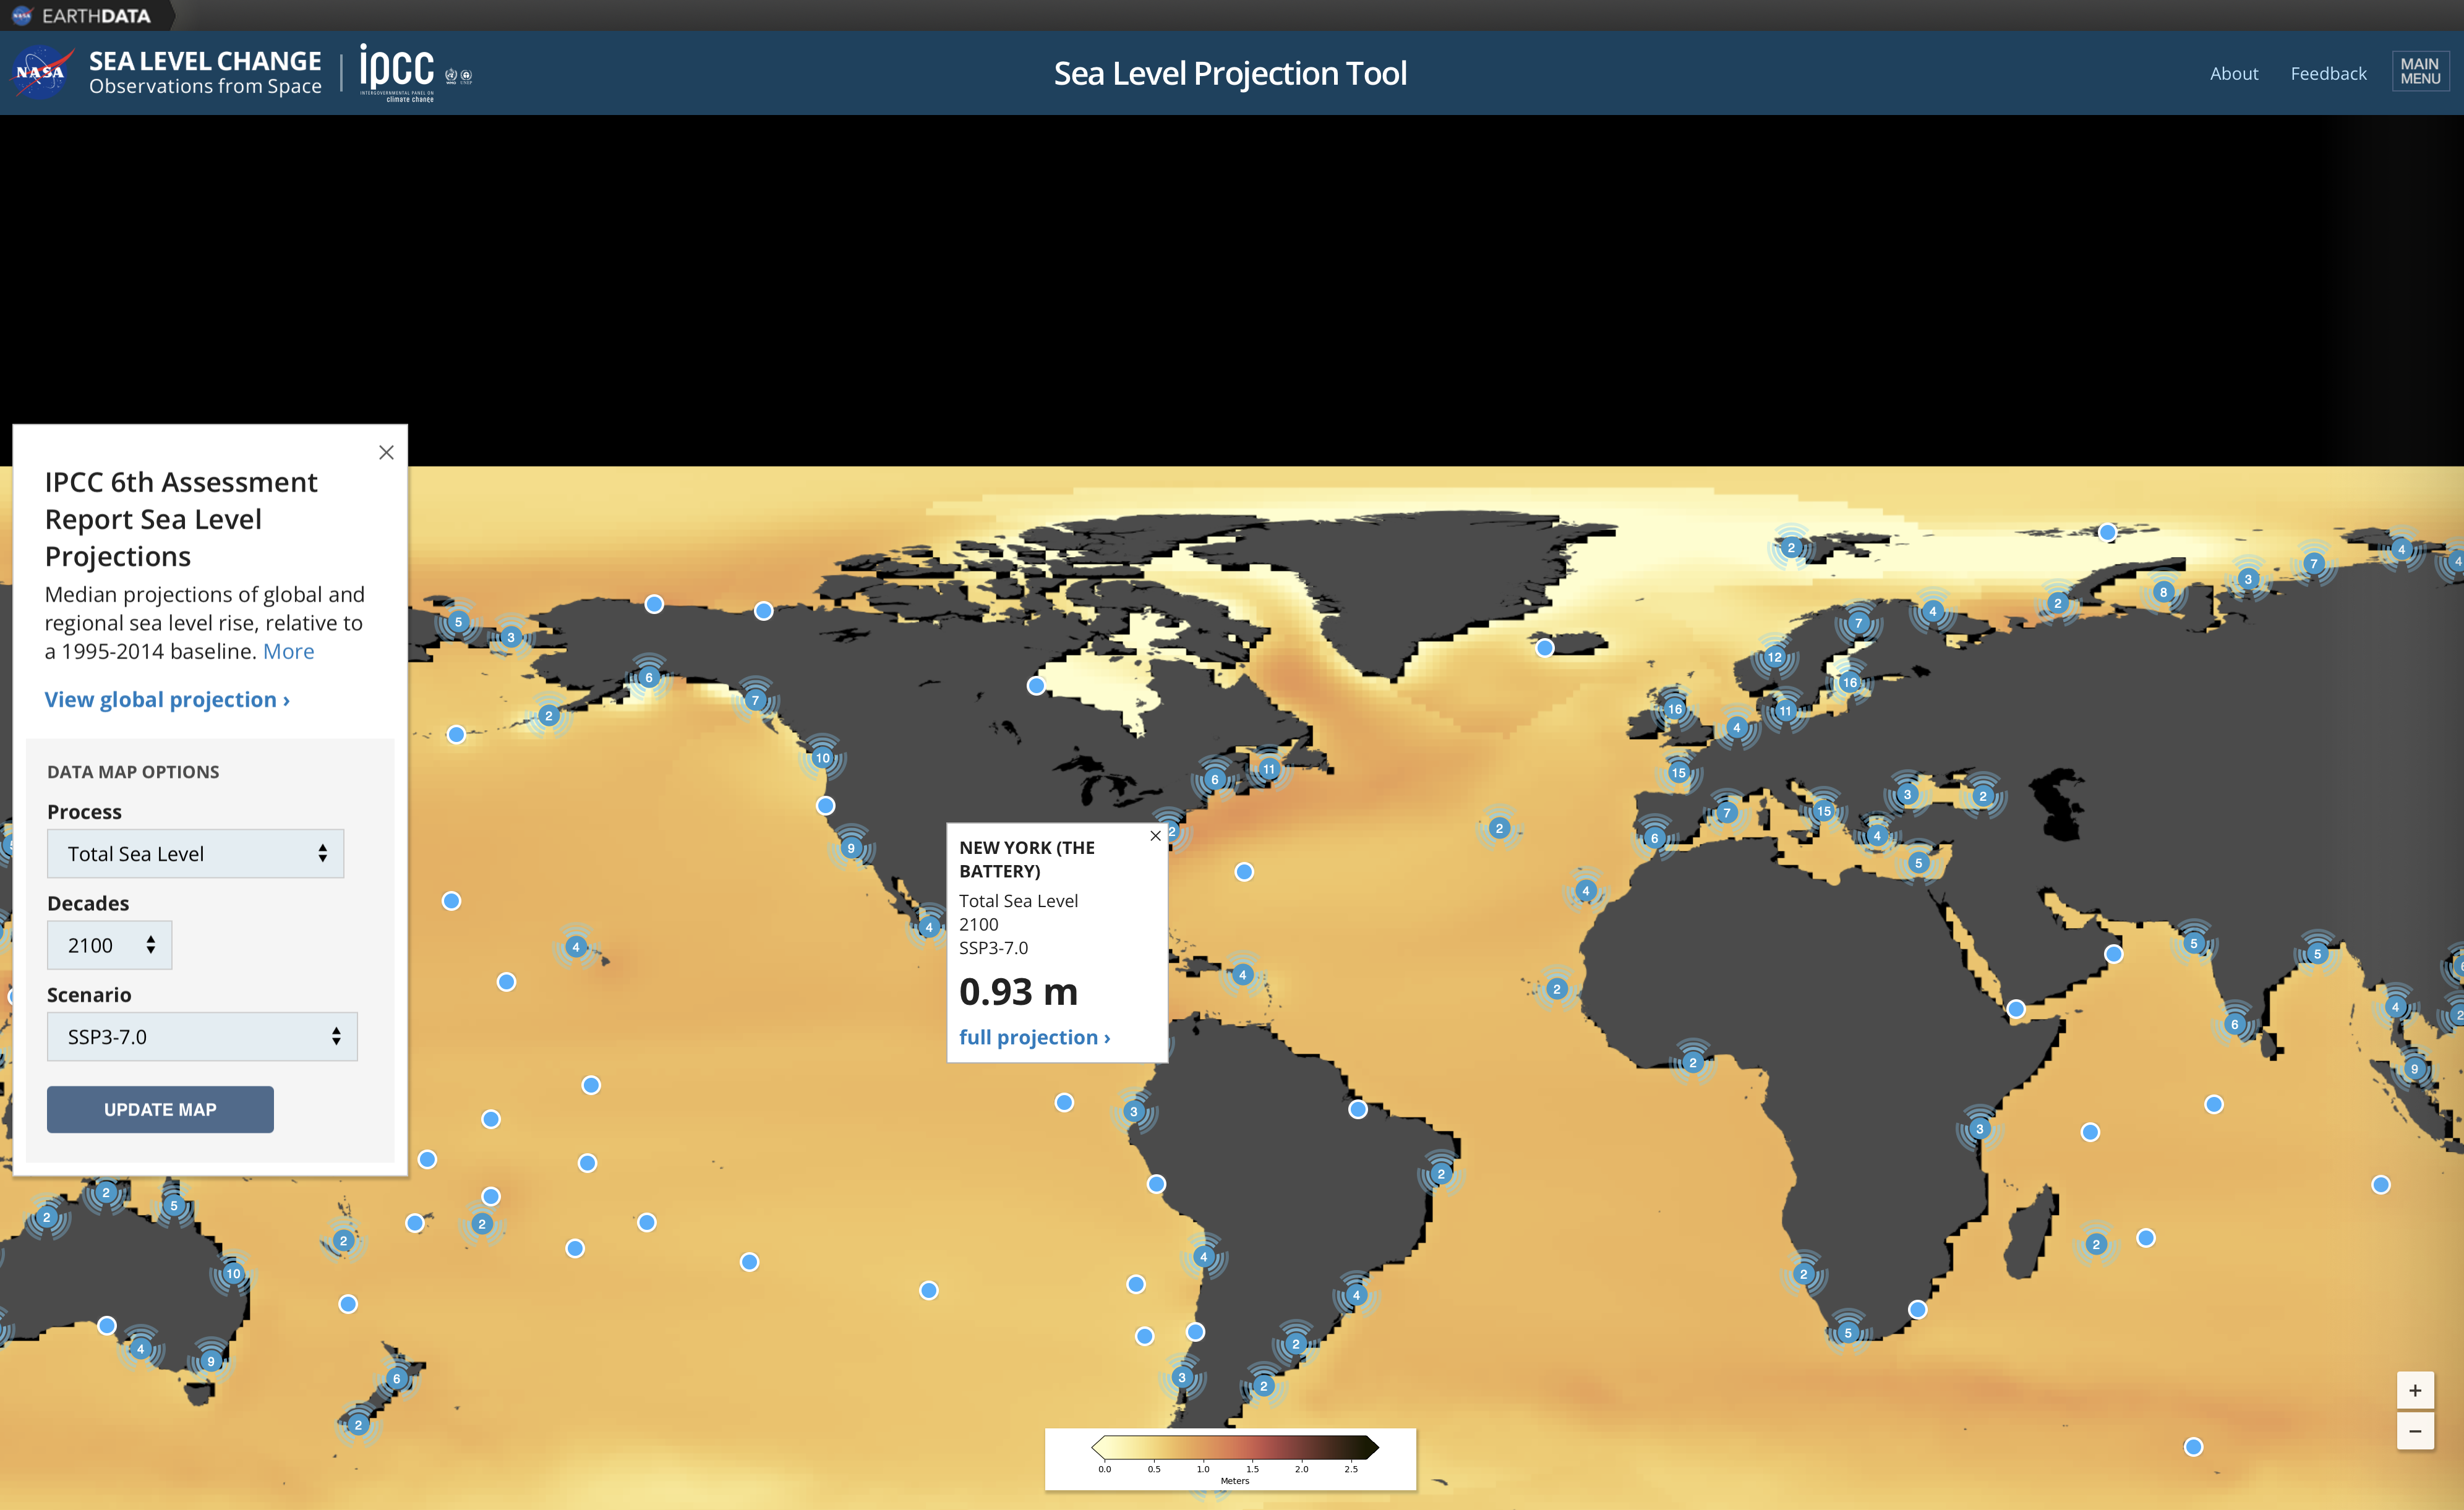
\includegraphics[width=0.55\columnwidth]{extraplots/nasa-sea-level-projection-tool.png}
  
 \vspace{0.1in}
%\begin{block}{IPCC Fourth Assessment Report: Climate Change 2007}
%  {\small
%    {\em [T]he uncertainty in the projections of the land ice
%      contributions [to sea level rise] is dominated by the various
%      uncertainties in the land ice models themselves
%      ... rather than in the temperature projections.''} %[10.A.6]
%  }
 %\end{block}
 \begin{itemize}
 \item Several port cities will be at risk from coastal
   flooding in the future.
 \item Ice flowing from ice sheets to ocean is primary contributor
   to sea level rise.
 \end{itemize}

 \begin{itemize}
  \item [] \scriptsize{Details in: Masson-Delmotte, V. et al. ``IPCC,
    2021: Summary for Policymakers. In: Climate Change 2021: The
    Physical Science Basis. Contribution of Working Group I to the
    Sixth Assessment Report of the Intergovernmental Panel on Climate
    Change'', Cambridge University Press. In Press.}
  \end{itemize}

 
 
\end{frame}
%-----------
%--------------------------------------------------------
\begin{frame}
  %\frametitle{Motivations: Infer basal sliding in an ice sheet model and characterize the associated uncertainties}
  \frametitle{Challenges and the need to exploit problem structure}

  Severe mathematical and computational challenges place significant
  barriers on improving predictability of ice sheet flow models, e.g.,
  
  \begin{minipage}{.6\columnwidth}
    \begin{itemize}
    \item complex and very high-aspect ratio (thin) geometry,
    \item highly nonlinear and anisotropic rheology,
    \item extremely ill-conditioned and large-scale linear and
      nonlinear algebraic systems that arise upon discretization,
    \item uncertain basal sliding parameter, basal topography,
      geothermal heat flux, and rheology,
    \item modeling error, etc.
    \end{itemize}
    
  \end{minipage}\hfill
  \begin{minipage}{.4\columnwidth}
    \begin{figure}\centering
      \includegraphics[width=0.99\columnwidth]{extraplots/antarctica_uobs_rotsurface_larger}\\
      \vspace{0.2in}
      \centering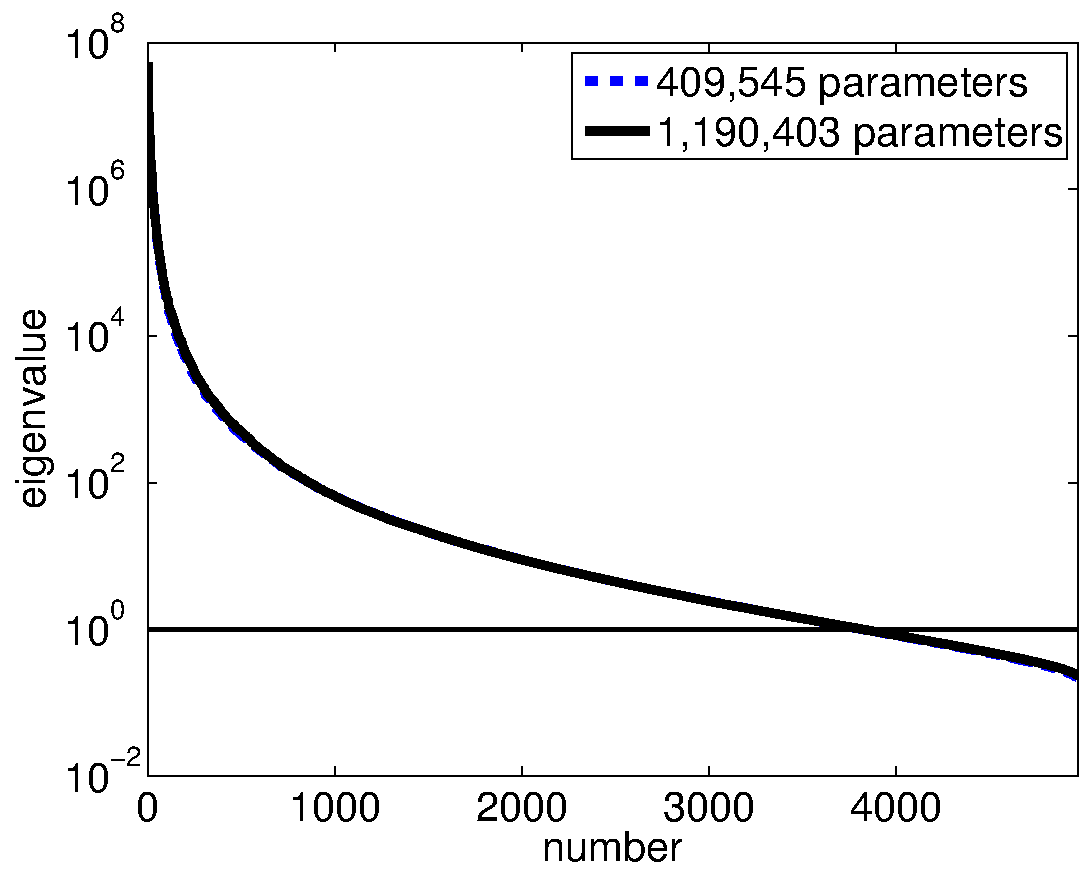
\includegraphics[width=0.65\columnwidth]{extraplots/spec_ppmisfit_hess_coarseandfine_new.pdf}
    \end{figure}
  \end{minipage}

  \vspace{0.1in}
  \begin{itemize}
  \item [] \scriptsize{Details in: T. Isaac, N. Petra, G. Stadler, and
    O. Ghattas. ``Scalable and efficient algorithms for the
    propagation of uncertainty from data through inference to
    prediction for large-scale problems, with application to flow of
    the Antarctic ice sheet'', Journal of Computational Physics, 296,
    348-368 (2015). {\it Selected as the 2019 SIAM Activity Group on
    Computational Science and Engineering Best Paper.}}
  \end{itemize}

  %``To address the challenges of learning models from data in the
  %large-scale setting of partial differential equations, we must
  %exploit the low-dimensional structure of the map from inputs to
  %outputs.'' (O. Ghattas and K. Willcox, ``Learning physics-based
  %models from data: perspectives from inverse problems and model
  %reduction'', Acta Numerica (2021).)

\end{frame}
%-------------------------------------------------------------------
\begin{frame}
  %\frametitle{Motivations: Infer basal sliding in an ice sheet model and characterize the associated uncertainties}
  \frametitle{How can we address (some of) these challenges?}

  %To address some of these challenges, we
  %\vspace{0.05in}
  \begin{minipage}{.6\columnwidth}
    \begin{itemize}
    \item Learn models from data, i.e., infer unknown/uncertain
      parameters from available data, e.g., satellite measurements of
      surface ice flow velocity ({\bf statistical inverse problems
        governed by PDEs})
    \item Apply/adapt/design fast, mesh-independent, structure
      exploiting, inner-product- and additional uncertainty-aware
      methods ({\bf scalable, robust and efficient algorithms})
    \item Collect data in an optimal way in order to minimize the
      uncertainty in the inferred parameters or in some predictive
      quantity of interest ({\bf optimal experimental design}).
    \end{itemize}
  \end{minipage}\hfill
  \begin{minipage}{.4\columnwidth}
    \begin{figure}\centering
      \includegraphics[width=0.99\columnwidth]{extraplots/antarctica_uobs_rotsurface_larger}\\
      \vspace{0.2in}
      \centering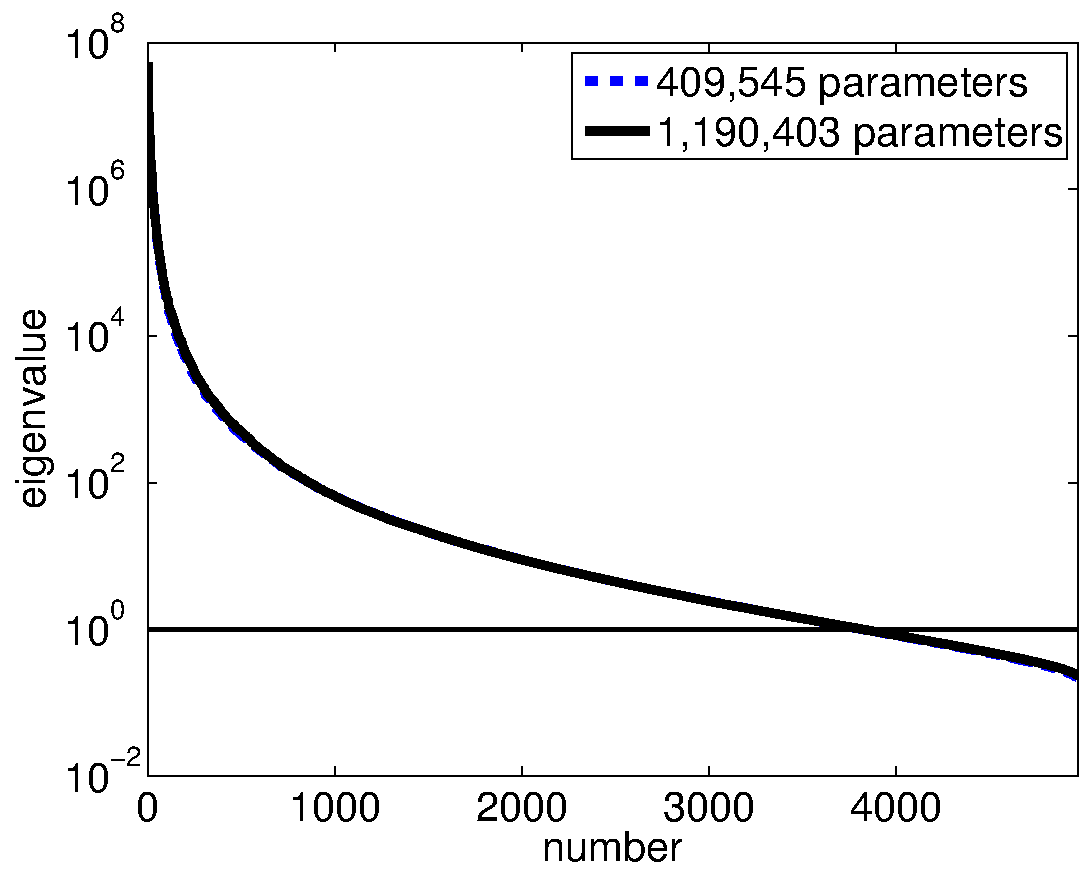
\includegraphics[width=0.65\columnwidth]{extraplots/spec_ppmisfit_hess_coarseandfine_new.pdf}
    \end{figure}
  \end{minipage}

  \vspace{0.15in}
  \begin{itemize}
  \item [] \scriptsize{Details in: O. Ghattas and
    K. Willcox. ``Learning physics-based models from data:
    perspectives from inverse problems and model reduction'', Acta
    Numerica, Cambridge University Press (2021).}
  \end{itemize}

  %``To address the challenges of learning models from data in the
  %large-scale setting of partial differential equations, we must
  %exploit the low-dimensional structure of the map from inputs to
  %outputs.'' (O. Ghattas and K. Willcox, ``Learning physics-based
  %models from data: perspectives from inverse problems and model
  %reduction'', Acta Numerica (2021).)

\end{frame}
%% -------------------------------------------------------------------
%\begin{frame}
%  \frametitle{The forward problem}
%  \framesubtitle{Nonlinear Stokes ice sheet model (for viscous, shear-thinning, incompressible fluid)}
%
%  Invoking the balance of mass and linear momentum:
%  %  \small
%  \vskip 0.1in
%  \begin{minipage}{.4\columnwidth}
%    \begin{alignat}{2}\nonumber
%      % mass
%      % momentum
%      - \gbf{\nabla} \cdot \left[ 2\gamma(\gbf{u}, n) \, \edot_{\gbf{u}}
%      -\gbf{I}p \right] &= \rho \gbf{g} \ & &\text{ in }
%      \Omega \nonumber\\
%      \gbf{\nabla} \cdot \gbf{u} &= 0 & &\text{ in }
%      \Omega \nonumber\\
%      \gbf{\sigma}_{\gbf{u}} \gbf{n} &= \gbf{0}  & &\text{ on }
%      \Gamma_{\!\scriptsize t}  \nonumber\\
%      \gbf{u}\cdot \gbf{n} = 0, \, \gbf T \gbf{\sigma}_{\gbf{u}} \gbf{n} +
%      {\exp(\beta)}\gbf{T}\gbf{u} &= \gbf{0}
%      & &\text{ on } \Gamma_{\!\scriptsize
%        b}\nonumber
%    \end{alignat}
%%\gbf{u}\cdot \gbf{n} = 0, \, \gbf T \gbf{\sigma}_{\gbf{u}} \gbf{n} +
%%      \tcr{\exp(\beta)} |\gbf{T}\gbf{u}|^{m-1}\gbf{T}\gbf{u} &= \gbf{0}
%%      & &\text{ on } \Gamma_{\!\scriptsize
%%        b}\nonumber
%%%    \hskip 0.75in + \; \text{additional B.C.s}
%  \end{minipage}\hfill
%  \begin{minipage}{.4\columnwidth}
%    \begin{figure}\centering
%      \includegraphics[width=0.99\columnwidth]{../extraplots/ymir/antarctica_uobs_rotsurface_larger}
%    \end{figure}
%  \end{minipage}
%  \\[3.5ex]
%  \begin{minipage}{0.565\columnwidth}
%    \begin{center}
%      \begin{minipage}{\columnwidth}
%	\vfill
%	\begin{itemize}
%	\item $\gbf u$ ice flow velocity, $p$ pressure
%	\item $\gbf{\sigma}_{\gbf{u}} = -\gbf{I}p + 2\gamma(\gbf{u},
%          n)\edot_{\gbf{u}}$ stress tensor
%	\item $\edot_{\gbf{u}} = \frac12 (\gbf{\nabla u} + \gbf{\nabla
%          u}^T)$ strain rate tensor
%        \item $\gamma(\gbf u, {n}) = \frac12 {A}^{-\frac{1}{{n}}} \;
%          \secinve^{\frac{1-{n}}{2{n}}}$ effective viscosity
%        \item $\secinve = \frac12 \mathrm{tr}(\edot_{\gbf{u}}^2)$
%          second invariant of the strain rate tensor
%	\end{itemize}
%        \vfill
%      \end{minipage}
%      %}
%    \end{center}
%  \end{minipage}\hfill
%  \begin{minipage}{0.43\columnwidth}
%    \begin{itemize}
%    \item $\rho$ density, $\gbf g$ gravity
%    \item $\gbf n$ unit normal vector
%    \item ${\beta}$ log basal sliding coefficient
%      %\item $m$ the basal sliding exponent
%    \item $ \gbf{T} = \gbf I - \gbf n \otimes \gbf  n$
%      tangential operator
%    \item $\Gamma_{\!\scriptsize t}$ and $\Gamma_{\!\scriptsize b}$
%      top and base boundaries
%    \end{itemize}
%    \vfill
%  \end{minipage}\\[1ex]
%
%\end{frame}
%
%%-----------------------------------------------------------
\begin{frame}
  \frametitle{The inverse problem}
  %\framesubtitle{\hip Model}

  %\begin{itemize}
  %  \uncover<1-2>{
  %\item \alert{The forward problem}: Given some input parameter field
  %  (coefficient, right hand side, initial condition, boundary
  %  condition, etc.)  $\tcr{\ipar}$ solve
  %  \begin{align*}
  %    r(\tcb{\istate}, \tcr{\ipar}) = 0,
  %  \end{align*}
  %  for $\tcb{\istate}$, where $r: \mathcal{V}\times\iparspace \to
  %  \mathcal{V}^*$ represents the PDE problem with $\mathcal{V}$ a
  %  suitable Hilbert space of functions defined on a bounded domain
  %  $\D \subset \R^d$, and $\iparspace \subseteq L^2(\D)$.
  %  }
  %  \uncover<2-2>{
    % \item \alert{The inverse problem}
  %consists of
  Use available observations/data $\obs$ to infer the
  values of the unknown parameter field $\tcr{\ipar}$ that
  characterize a physical process modeled by PDEs, i.e.,
  %Mathematically
      %this inverse relationship is expressed as
      \begin{align*}
        \obs = \ff(\tcr{\ipar}) + \vec{\eta}.
      \end{align*}
      \vspace{-0.2in}
      \begin{itemize}
      \item The map $\ff: \iparspace \to \mathbb{R}^q$ is the so-called
        {\it parameter-to-observable} map.
      \item Evaluations of $\ff$ involve the solution of the Stokes
        PDE given $\tcr{\ipar}$, followed by the application of an
        observation operator $\mathcal{B}: \mathcal{V} \to
        \mathbb{R}^q$ to extract the observations from the state.
      \item $\vec{\eta}$ accounts for noisy measurements and model
        errors and is modeled as $\vec{\eta} \sim
        \GM{\vec{0}}{\ncov}$, i.e., a centered Gaussian at $\vec{0}$
        with covariance $\ncov$.
      \end{itemize}
   % }
  %\end{itemize}
\end{frame}
%-----------------------------------------------------------
\begin{frame}
  \frametitle{Bayesian formulation of the inverse problem}

   Describes probability of all models that are consistent with the
   observations/data and any prior knowledge about the parameters:
    %\begin{block}
    \begin{equation*}
      d\mupost \propto \exp\Big\{-\half \| \ff(\tcr{\ipar}) -
      \vec{d} \|^2_{\ncov^{-1}} -\half\| \tcr{\ipar} - \iparpr\|^2_{\Cprior^{-1}} \Big\}.
    \end{equation*}
    %\end{block}
    \begin{itemize}
    \item The first term in the exponential is the negative log-likelihood.
    \item The second term represent the negative log-prior (e.g.,
      Gaussian prior, i.e., $\tcr{\ipar} \sim \GM{\iparpr}{\Cprior}$).
    \end{itemize}

    \begin{block}{Goal:}
      \begin{itemize}
      \item characterize the posterior statistically (MAP point, mean, covariance, etc.)
      \item for functions $\bs m$ (large vectors after discretization)
      \item for expensive $\ff(\cdot)$
      \item exploit connection to PDE-constrained optimization
      \end{itemize}
    \end{block}
\end{frame}
%--------------------------------------------------------------------
\begin{frame}
  \frametitle{Inverse problems governed by PDEs}
  %\framesubtitle{\hip Model}
  \begin{itemize}
    \uncover<1-2>{
    \item The \emph{maximum a posteriori} (MAP) point $\iparmap$ is
    defined as the parameter field that maximizes the posterior
    distribution: %It can be obtained by solving the following
    %deterministic optimization problem
    \begin{align*}
      \iparmap :&= \argmin_{\tcr{\ipar} \in \iparspace} (- \log
      d\mupost(\tcr{\ipar}) ) \\
      &= \argmin_{\tcr{\ipar} \in \iparspace} \half \|
      \ff(\tcr{\ipar}) - \vec{d} \|^2_{\ncov^{-1}} + \half\| \tcr{\ipar} -
      \iparpr\|^2_{\Cprior^{-1}} \\
      &=\argmin_{\tcr{\ipar} \in \iparspace} \half \|
      \mathcal{B}(\tcb{\istate}) - \vec{d} \|^2_{\ncov^{-1}} + \half\| \tcr{\ipar} -
      \iparpr\|^2_{\Cprior^{-1}},
    \end{align*}
    where $\tcb{\istate}$ solves the forward Stokes (PDE) problem. %$r(\tcb{\istate}, \tcr{\ipar}) = 0$.
    %We note that, the prior information plays the role of Tikhonov
    %regularization in \eqref{eq:optpb}; in fact the deterministic
    %optimization problem \eqref{eq:optpb} is the same as
    %\eqref{eq:map_continuum} for the choice $\R(\ipar) = \half\| m -
    %\iparpr\|^2_{\Cprior^{-1}}$.  The Hessian $\mathcal{H}(\iparmap)$
    %of the negative log-posterior evaluated at $\iparmap$ plays a
    %fundamental role in quantifying the uncertainty in the inferred
    %parameter. In particular, this indicates which directions in the
    %parameter space are most informed by the data
    %\cite{Bui-ThanhGhattasMartinEtAl13}.
    }
    \uncover<2-2>{
    \item When $\iFF$ is
    linear, due to the particular choice of prior and noise model, the
    posterior measure is Gaussian, $\GM{\iparmap}{\Cpost}$
    \begin{equation*}
      \iparmap = \Cpost(\iFFadj\ncov^{-1}\obs + \Cprior^{-1}\iparpr),
      \qquad 
      \Cpost = \mathcal{H}^{-1} = (\iFFadj \ncov^{-1} \iFF + \Cprior^{-1})^{-1},
    \end{equation*}
    where $\iFFadj:\R^q \to \iparspace$ is the adjoint of $\iFF$, and
    $\mathcal{H}$ is the Hessian (second derivative) of the
    negative-log posterior.
    %\vspace{0.15in}
    \item {\bf Note:} In the general case of nonlinear
      parameter-to-observable map $\iFF$ the posterior distribution is
      not Gaussian. %In this case
      %one would need to use sampling to characterize the posterior.
     }
  \end{itemize}
\end{frame}
%%%% --------------------------------------------------------------------
%\begin{frame}
%  \frametitle{Data$\rightarrow$Inference$\rightarrow$Prediction}
%
%  \begin{itemize}
%  \item While one can formulate a {\bf data-to-prediction framework}
%    to {\bf quantify uncertainties from data to inferred model
%      parameters to predictions} with an underlying model of
%    non-Newtonian ice sheet flow, attempting to execute this framework
%    for the Antarctic ice sheet (or other large-scale complex models)
%    is intractable for high-dimensional parameter fields using current
%    algorithms.
%    \vspace{0.05in}
%    
%  \item Yet, quantifying the uncertainties in predictions of ice sheet
%    models is essential if these models are to play a significant role
%    in projections of future sea level.
%    \vspace{0.05in}
%    
%  \item {\bf Goal:} design an integrated framework and efficient,
%    scalable algorithms (under Gaussian approximations of the
%    posterior and prediction) for carrying out this data-to-prediction
%    process.
%    \vspace{0.05in}
%    
%    %Two key ideas are needed to produce such scalable
%    %algorithms. First, we use Gaussian approximations of both the
%    %posterior pdf that results from Bayesian solution of the inverse
%    %problem of inferring ice sheet parameter fields from satellite
%    %observations of surface velocity, as well as the pdf resulting
%    %from propagating the uncertain parameter fields through the
%    %forward ice sheet model to yield predictions of present-day mass
%    %flux into the ocean. This is accomplished by linearizing the
%    %parameter-to-observable map as well as the parameter-to-prediction
%    %map around the maximum a posterior point.
%    
%  \item {\bf Scalable:} the cost-measured in number of PDE solves-is
%    independent of not only the number of processor cores, but
%    importantly the state variable dimension, the parameter dimension,
%    and the data dimension.
%  \end{itemize}
%  
%  \begin{itemize}
%  \item [] \scriptsize{Details in: T. Isaac, N. Petra, G. Stadler, and
%    O. Ghattas. ``Scalable and efficient algorithms for the
%    propagation of uncertainty from data through inference to
%    prediction for large-scale problems, with application to flow of
%    the Antarctic ice sheet'', Journal of Computational Physics, 296,
%    348-368 (2015).}
%  \end{itemize}
%\end{frame}
%
%------------------------
%---------------------------------------------------------------------------------%
\begin{frame}
  \frametitle{The Hessian (of the negative log posterior) plays a
    critical role in inverse problems}
  \begin{itemize}
  \item Its spectral properties characterize the degree of
    ill-posedness.
  \item The Hessian drives Newton-type optimization algorithms for
    solving the inverse problem.
  \item The inverse of the Hessian locally characterizes the uncertainty
    in the solution of the inverse problem (under the Gaussian
    assumption, it is precisely the posterior covariance matrix).
  \item \alert{Goal:} rapidly perform linear algebraic operations, i.e.,
    manipulation of the Hessian (and its square root and inverse)
    actions needed by sampling or CG solvers, hence \alert{seek
      approaches to approximate the Hessian(-applies)}.
  \item These approximations can then be used as
    \alert{pre-conditioners}, and to \alert{build MCMC proposals} based
    on local Gaussian approximations.
  \end{itemize}
\end{frame}
%---------------------------------------------------------------------------------%
\begin{frame}
\frametitle{Scalability of an ice sheet inverse solver}
\framesubtitle{Inexact Newton-CG}

  \only<1>{
\begin{table}
\begin{center}
  \small
  \label{tbl:performance}
  \begin{tabular}{|r|r|r|r|r|r|}
    \hline
        {\bf \#sdof}    &   {\bf \#pdof}   &    {\bf  \#N}   &  {\bf  \#CG}
        & {\bf  avgCG}   &  {\bf \#Stokes} \\
        \hline
        %69101 &   7485 &  36 &  2534 &    70 & 1609 &     6713 \\
        95,796 &  10,371 &  42 &  2718 &    65         &     7031 \\
                                              % 1553 &    
        233,834 &  25,295 &  39 &  2342 &    60        &     6440 \\
                                              % 1717 &
        848,850 &  91,787 &  39 &  2577 &    66        &     6856 \\
                                              % 1663 &
        3,372,707 & 364,649 &  39 &  2211 &    57       &     6193 \\
                                              % 1732 
        %5667771 & 365709 &  43 &  2139 &    50 &     1978 &     6299\\
        22,570,303 & 1,456,225 &  40 &  1923 &    48     &     5376\\
                                              % 1490
        \hline
  \end{tabular}
\end{center}
\end{table}
  }
  \only<2>{
\begin{table}
\begin{center}
  \small
  %\caption{Scalability of inverse solver}
  \label{tbl:performance}
  \begin{tabular}{|r|r|r|r|r|r|}
    \hline
        {\bf \#sdof}    &   {\bf \#pdof}   &    {\bf  \#N}   &  {\bf  \#CG}
        & {\bf  avgCG}   &  {\bf \#Stokes} \\
        \hline
        %69101 &   7485 &  36 &  2534 &    70 & 1609 &     6713 \\
        95,796 &  10,371 &  42 &  2718 &    65         &     {\bf\alert{7031}} \\
                                              % 1553 &    
        233,834 &  25,295 &  39 &  2342 &    60        &     {\bf\alert{6440}} \\
                                              % 1717 &
        848,850 &  91,787 &  39 &  2577 &    66        &     {\bf\alert{6856}} \\
                                              % 1663 &
        3,372,707 & 364,649 &  39 &  2211 &    57       &     {\bf\alert{6193}} \\
                                              % 1732 
        %5667771 & 365709 &  43 &  2139 &    50 &     1978 &     6299\\
        22,570,303 & 1,456,225 &  40 &  1923 &    48     &     {\bf\alert{5376}}\\
                                              % 1490
        \hline
  \end{tabular}
\end{center}
\end{table}
  }
  
\small
\begin{itemize}
\item {\bf \#sdof}: number of degrees of freedom for the
  state variables;
\item {\bf \#pdof}: number of degrees of freedom for the
  inversion parameter field;
\item {\bf \#N}: number of Newton iterations;
\item {\bf \#CG}, {\bf avgCG}: total and average (per Newton
  iteration) number of CG iterations;
\item {\bf \#Stokes}: total number of
  linear(ized) Stokes solves (from forward, adjoint, and incremental
  forward and adjoint problems)
\end{itemize}

\begin{itemize}
\item [] \scriptsize{Details in: T. Isaac, N. Petra, G. Stadler, and
  O. Ghattas. {\em Scalable and efficient algorithms for the
    propagation of uncertainty from data through inference to
    prediction for large-scale problems, with application to flow of
    the Antarctic ice sheet}, Journal of Computational Physics, 296,
  348-368 (2015).}
\end{itemize}

\end{frame}

%---------------------------------------------------------------------------------%
\begin{frame}
\frametitle{Low-rank approximation of the Hessian of the likelihood}
% (Gauss-Newton)

\framesubtitle{Under the assumption of Gaussian noise and linearized
  parameter-to-observable map}

\begin{itemize}

\item Invoke low-rank approximation  given by the inverse of the Hessian:
  \begin{minipage}{0.9\textwidth}
  \begin{block}{}
    %\vspace{-0.5cm} 
    \[
    \postcov = \Hmatrix^{-1} =
    \left( \prcov \Hmatrix_{\text{misfit}} + \bs{I} \right)^{-1} \prcov
    \approx \prcov - \bs{W}_r \bs{D}_r \bs{W}^T_r,
    %\left ( {\bs{F}^T\ncov^{-1}\bs{F}} + \prcov^{-1} \right)^{-1}
    %\approx \prcov^{1/2} (\bs{V}_r \bs{\Lambda}_r \bs{V}^T_r + \bs{I})^{-1}
    %\prcov^{1/2} 
    % - \bs{V}_r \bs{D}_r \bs{V}^T_r
    \]
  \end{block}
  \end{minipage}

  \vspace{0.15in} where $\bs{W}_r$ contains the largest $r$
  eigenvectors of $\prcov \Hmatrix_{\text{misfit}}$, and $\bs{D}_r =
  \diag(\lambda_i/(\lambda_i +1))\in \R^{r \times r}$, where
  $\lambda_i$ are eigenvalues of $\prcov \Hmatrix_{\text{misfit}}$.
%  the eigenvalue problem 
%$\bs{F}^T\ncov^{-1}\bs{F} \bs{v}_i = \lambda_i \prcov^{-1} \bs{v}_i $
  %, \bs{\Lambda}_r = \diag(\lambda_i)_{i=1}^r$
%  are truncated
%  generalized eigenvectors of the data misfit
%  Hessian, $\bs{D}_r =\diag(\lambda_i/(\lambda_i+1))$, and used
%  the Sherman-Morrison-Woodbury th. % to invert/factor.

%\item Spectrum of the prior-preconditioned likelihood Hessian for the
%  Arolla glacier (139 parameters, left) and
%  Antarctica (1.19M parameters, right) 
  %
  \end{itemize}
\begin{figure}[htb]
    \centering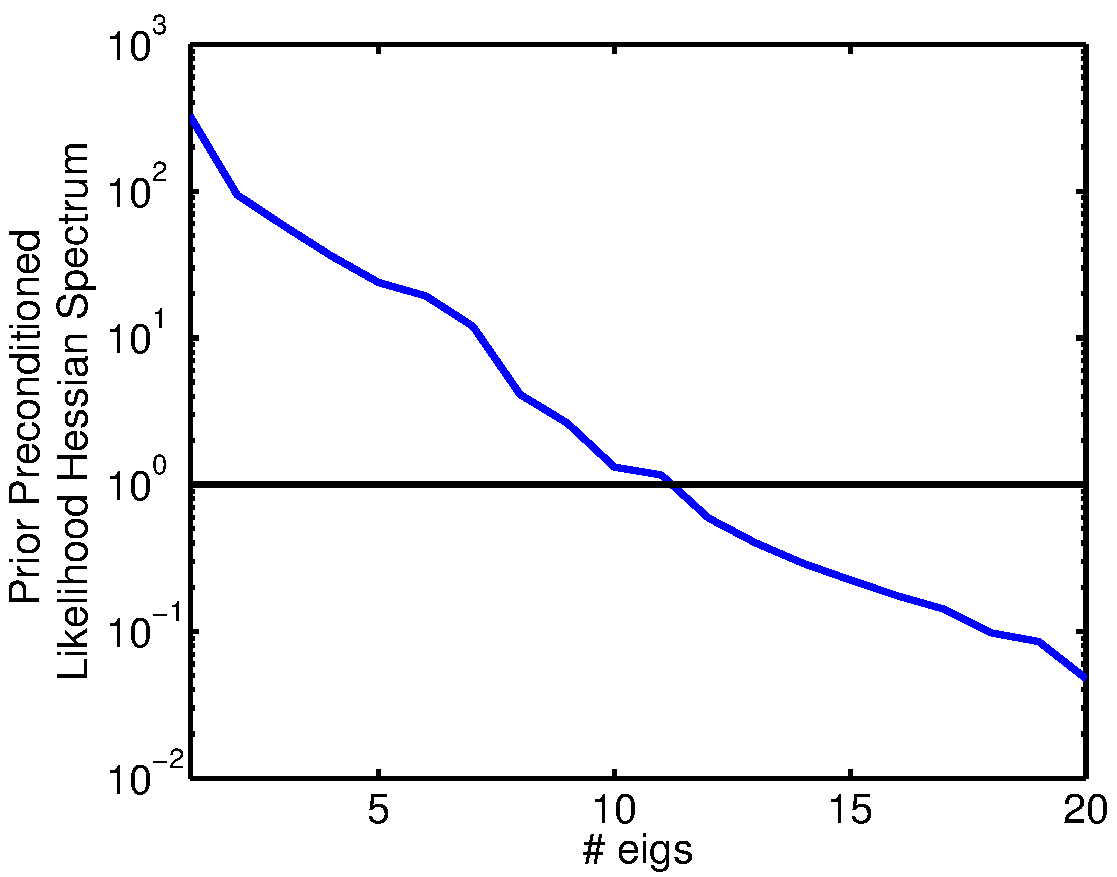
\includegraphics[width=0.35\textwidth]{extraplots/spectrum.pdf}
    \hspace{0.2in}
    \centering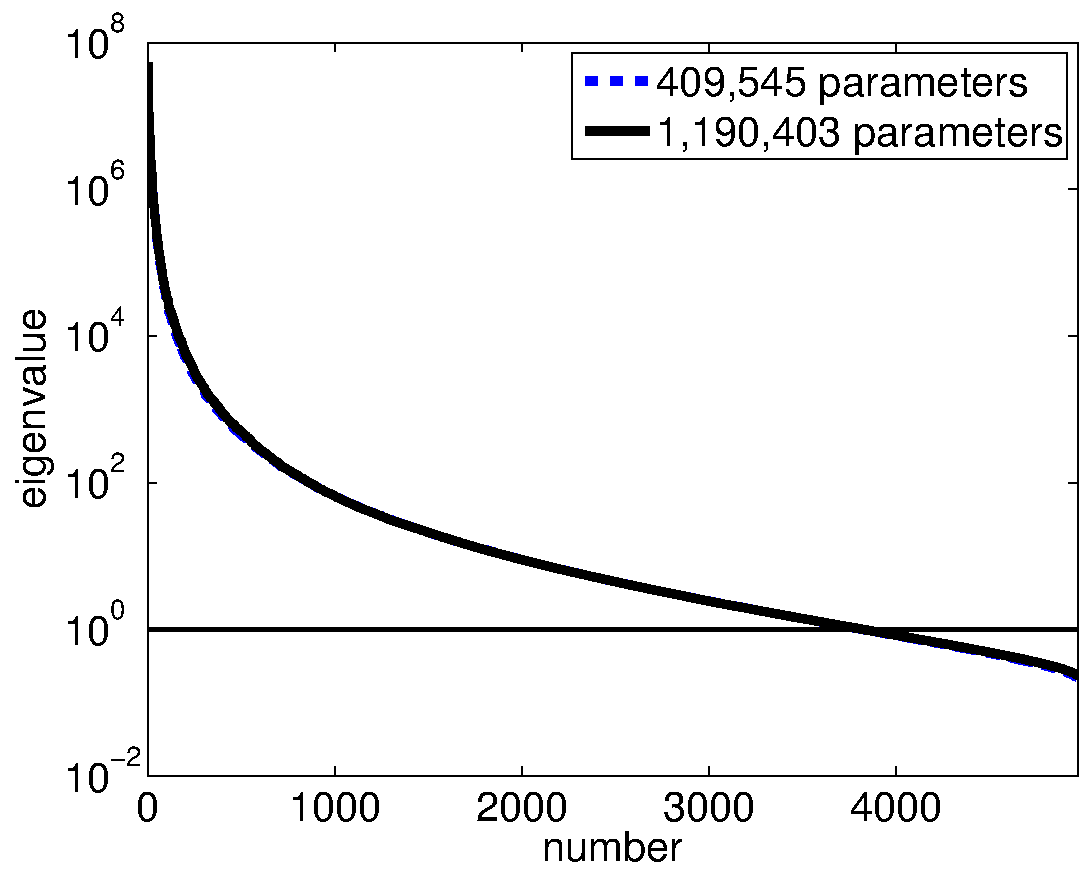
\includegraphics[width=0.35\textwidth]{extraplots/spec_ppmisfit_hess_coarseandfine_new.pdf}
  \end{figure}
  %
%\end{itemize}
\begin{center}
  The spectrum of the prior-preconditioned likelihood Hessian for the
  Arolla glacier (139 parameters, left) and Antarctica (1.19M
  parameters, right).
  \end{center}
\end{frame}

%---------------------------------------------------------------------------------%
\begin{frame}
\frametitle{MCMC sampling: stochastic Newton}
\framesubtitle{Performance results / Convergence diagnostics}
%\vspace{0.1in}
\small

\newcommand{\proposal}{\bs y}
\newcommand{\params}{\bs m}


\only<1>{
\begin{table}[t]
  \begin{center}
    %\def\firstrowcolor{}
    %\def\secondrowcolor{}
    %\only<1>{\def\firstrowcolor{\rowcolor{gray}}}
    %\only<2>{\def\secondrowcolor{\rowcolor{red}}}
    \begin{tabular}{|l|c|c|c|c|c|c|c|}
      \hline\hline
          {} & {\bfseries MPSRF} & {\bfseries IAT} & {\bfseries ESS} & {\bfseries
            MSJ} & {\bfseries ARR} & {\bfseries $\#$Stokes} & {\bfseries time (s)}\\
          \hline%\hline
          %\multicolumn{8}{|c|}{small noise case (more Gaussian) }\\
          %\hline
          %ind. sampler & 1.210 & 253 & 2075  & 1456 & 41 & 2783  & 139\\
          %frozen Hessian  & 1.001 & 6 & 84004 & 1390 & 40 & 72     & 4  \\
          %dynamic Hessian & 1.073 & 125 & 4032  & 565  & 17 & 1375 & 69\\
          %\hline
          %\multicolumn{8}{|c|}{large noise case (more non-Gaussian)}\\
          %\hline
          %SNIS  & 1.507 & 435 & 1207 & 280 & 9  & 4350 &  218\\
          %SNMAP  & 1.045 & 80 & 6563 & 190  & 6  & 960  & 48 \\
          SN & 1.348 & 600 & 875  & 64   & 2  & {\bf \alert{8400}} & 420 \\
          \hline\hline
    \end{tabular}
  \end{center}
\end{table}
}
\vspace{-0.05in}

\begin{columns}
  \begin{column}{0.45\columnwidth}
    \begin{itemize}
    \item {\bfseries MPSRF:} multivariate potential scale reduction factor
      \vspace{-0.02in}
    \item {\bfseries IAT:} integrated autocorrelation time
      \vspace{-0.02in}
    \item {\bfseries ESS:} effecitive sample size
      \vspace{-0.02in}
    \item {\bfseries MSJ:} mean squared jump distance
    \end{itemize}
  \end{column}
  \begin{column}{0.45\columnwidth}
    \begin{itemize}
    \item {\bfseries ARR:} average rejection rate
      \vspace{-0.02in}
    \item {\bfseries $\#$Stokes:} $\#$ of Stokes solves per independent sample
      \vspace{-0.02in}
    \item {\bfseries time:} time per independent sample
    \end{itemize}
  \end{column}
\end{columns}

\begin{columns}
  \hspace{0.26in}
  \begin{column}{0.95\columnwidth}
    \begin{itemize}
    \item {\bfseries Statistics:} 21 parallel chains (each 25k); $\#$
      samples: 525k; dof: 139; rank Hessian: 15
    %\item SNIS, SNMAP and SN are variants of the stochastic Newton
    %  MCMC method
    \end{itemize}
  \end{column}
  \begin{column}{0.5\columnwidth}
  \end{column}
\end{columns}

\vspace{0.05in}

%\vspace{-0.05in}
 \begin{align*}
   %\tcdb{q(\params_k,\proposal) =
     \mbox{ Proposal density: } \frac { \det \bs H^{1/2} }{(2\pi)^{n/2} }
      \exp \left( - \frac 12 \left( \proposal - \bs{\beta}_k + \bs H^{-1} \bs
      g \right) ^T \bs H \left( \proposal - \bs{\beta}_k + \bs H^{-1} \bs g \right)
      \right)
      %}
 \end{align*}
 
\begin{itemize}
\item [] \scriptsize{Details in: N. Petra, J. Martin, G. Stadler,
  O. Ghattas. {\em A computational framework for
    infinite-dimensional Bayesian inverse problems: Part
    II. Stochastic Newton MCMC with application to ice sheet inverse
    problems}, SIAM Journal on Scientific Computing, 2014}
\end{itemize}

\end{frame}
%---------------------------------------------------------------------
\begin{frame}
  \frametitle{Motivation to go beyond ``{\it global} low-rank approximation''}

    \begin{columns}
    \begin{column}{0.6\paperwidth}
        \begin{itemize}
  \item Existing Hessian approximations are based on low-rank approximation
    methods, which require computing twice as many linearized forward or
    adjoint partial differential equation (PDE) solves as the numerical
    rank of the Hessian.
    \vspace{0.05in}
  \item These methods are inefficient when the numerical rank of the Hessian
    is large, as is the case in continental scale ice sheet inverse
    problems.

  \end{itemize}
    \end{column}
    \begin{column}{0.35\paperwidth}
    \vspace{0.1in}
      \centering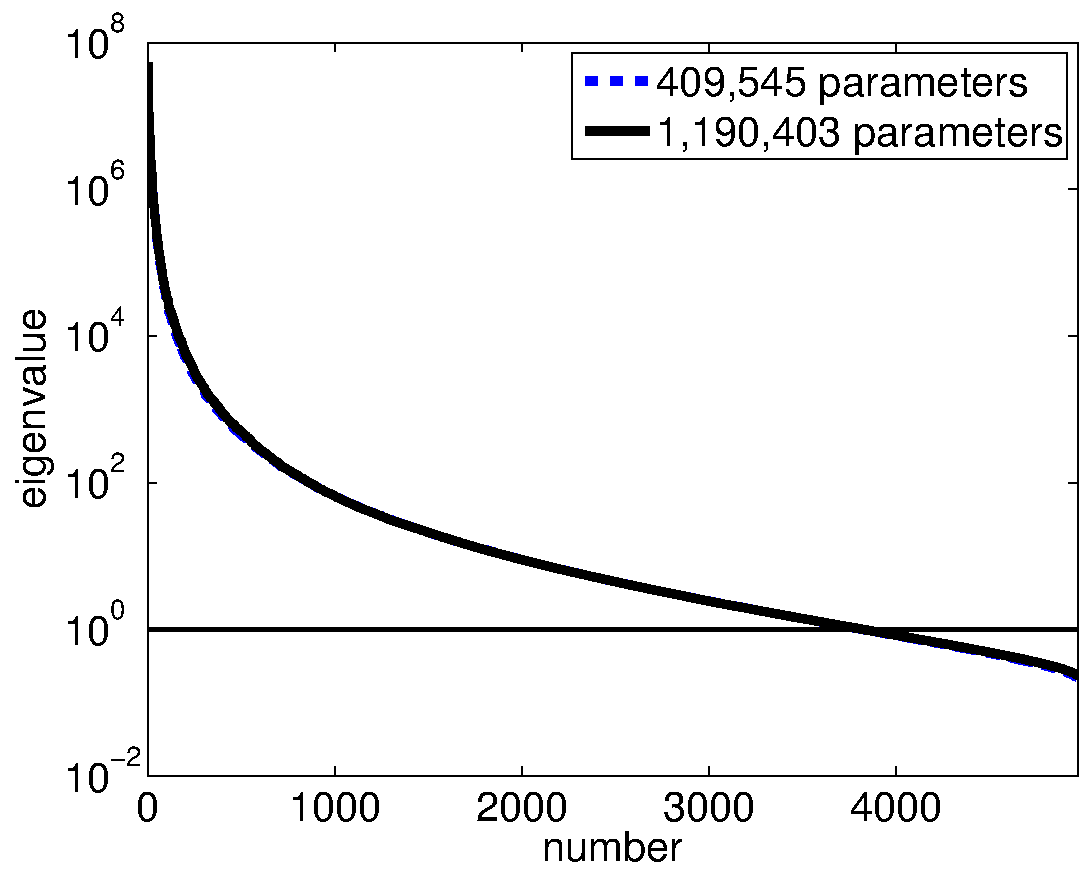
\includegraphics[width=0.95\columnwidth]{extraplots/spec_ppmisfit_hess_coarseandfine_new.pdf}
    \end{column}
    \end{columns}

    \vspace{0.1in}
    \begin{center}
      \alert{Our goal is to use additional structure combined with
        hierarchical matrix compression to reduce the
        computational cost of solving the (Bayesian) ice sheet inverse
        problem.}
    \end{center}
\end{frame}
%---------------------------------------------------------------------------
\begin{frame}
 \frametitle{Exploiting the problem structure}
 \framesubtitle{Local sensitivities}
 \center

 \begin{tikzpicture}
   \fill[red!90,nearly transparent] (5,0) -- (7,.5) -- (3,.5) -- (1,0) -- cycle;
   \draw [fill=red!40!white,opacity=1] (3,2.25) -- (3.5,2.25) -- (3.25,.25) -- cycle;
   \draw [fill=red] (3.25,2.25) circle (.25cm and 0.07cm);
   \draw (3.25,2.25) -- (2,3);
   \draw [thick] (2,3) node[above]{sensitivities, $\frac{\partial u}{\partial\beta_j}$};
   \draw[red,dashed] (7,.5) -- (3,.5) -- (1,0);
   \draw [fill=blue!40!white,opacity=1] (4.25,.25) -- (4.5,2.25) -- (4.75,.25) -- cycle;
   \draw [fill=blue] (4.5,.25) circle (.25cm and 0.07cm);
   \draw (4.5,.25) -- (2,-.5);
   \draw [thick] (2,-.5) node[below]{sensitivities, $\frac{\partial u_i}{\partial\beta}$};
   \draw (1,0) -- (5,0) -- (5,2) -- (1,2) -- (1,0);
   \draw  (5,2) -- (7,2.5) -- (3,2.5) -- (1,2);
   \draw  (7,2.5) -- (7,.5) -- (5,0);
   \draw  (5,2.25) -- (6,3) ;
   \draw [thick] (6,3) node[above]{measurements, $\boldsymbol{d}$};
   \draw[red]   (5.5,.25) -- (5.5,.125) ;
   \draw  (5.5,.125) -- (5.5,-.5) ;
   \draw [thick] (5.5,-.5) node[below]{parameter, $\beta(x)$};
   
   \draw[dashed] (3,.5) -- (3,2);
   \draw[blue,dashed] (3,2) -- (3,2.5);
   \fill[blue!90,nearly transparent] (5,2) -- (7,2.5) -- (3,2.5) -- (1,2) -- cycle;
 \end{tikzpicture}
%----------------------------------------------------------------------
\end{frame}
\begin{frame}
  \frametitle{Relevant literature}
  \scriptsize
  \vspace{-0.04in}
  \begin{itemize}
  \item {\bf (Global) low rank approximation}
    \vspace{0.02in}
    \begin{enumerate}
      \scriptsize
    \item Flath, Wilcox, Ak\c{c}elik, Hill, Van Bloemen Waanders, and
      Ghattas, {\it Fast algorithms for Bayesian uncertainty
        quantification in large-scale linear inverse problems based on
        low-rank partial Hessian approximations}, SISC, 2011.
    \item Halko, Martinsson, and Tropp, {\it Finding structure with
      randomness: Probabilistic algorithms for constructing
      approximate matrix decompositions}, SIAM review, 2011.
    \item Ghattas and Willcox, {\it Learning physics-based models from
      data: perspectives from inverse problems and model reduction},
      Acta Numerica, 2021.
    \end{enumerate}
    \vspace{-0.02in}
  \item {\bf Hierarchical (H-)matrix approximations}
    \vspace{0.02in}
    \begin{enumerate}
      \scriptsize
    \item Hackbusch, {\it Hierarchical matrices: algorithms and
      analysis}, Springer, 2015.
    \item Martinsson, {\it Fast direct solvers for elliptic PDEs},
      SIAM, 2020.
    \item Lin, Lu, and Ying, {\it Fast construction of hierarchical
      matrix representation from matrix-vector multiplication},
      JCP,2011.
    \item Ambartsumyan, Boukaram, Bui-Thanh, Ghattas, Keyes, Stadler,
      Turkiyyah, and Zampini, {\it Hierarchical matrix approximations
        of Hessians arising in inverse problems governed by PDEs},
      SISC, 2020.
    \item Hartland, Stadler, Perego, Liegeois, and Petra, {\it
      Hierarchical off-diagonal low-rank approximation of Hessians in
      inverse problems, with application to ice sheet model
      initialization}, Inverse Problems, 2023.
    \item Chen, Anitescu, {\it calable Physics-based Maximum
      Likelihood Estimation using Hierarchical Matrices}, JUQ, 2023.
    \end{enumerate}
    \vspace{-0.02in}
  \item {\bf Point spread function approximation combined with
    hierarchical matrix (H-matrix) approximation}
    \vspace{0.02in}
    \begin{enumerate}
      \scriptsize
    \item Gentile, Courbin, and Meylan, {\it Interpolating point
      spread function anisotropy} Astronomy \& Astrophysics, 2013.
    \item Escande and Weiss, {\it Approximation of integral operators using product-convolution
expansions}, Journal of Mathematical Imaging and Vision, 2017.
    \item Alger, {\it Data-scalable Hessian preconditioning for
      distributed parameter PDE-constrained inverse problems}, PhD
      thesis, The University of Texas at Austin, 2019.
    \end{enumerate}
  \end{itemize}
\end{frame}
%---------------------------------------------------------------------
\begin{frame}
  \frametitle{Hierarchical matrices ($\mathcal{H}$-matrices)}

    \begin{columns}
    \begin{column}{0.7\paperwidth}
       \begin{itemize}
		\item Matrix is reordered and subdivided recursively
		\item Many off-diagonal blocks are low-rank
		\item Overall matrix may be high rank
		\item $O(N \left(\log N\right)^a)$ complexity matrix operations, $a \in \{0,1,2,3\}$
		\begin{itemize}
			\item matrix-vector products, matrix-matrix addition, matrix-matrix multiplication, matrix factorization, matrix inversion, ...
		\end{itemize}
	\end{itemize}
    \end{column}
    \hspace{-0.4in}
    \begin{column}{0.3\paperwidth}
    \vspace{0.1in}
      \centering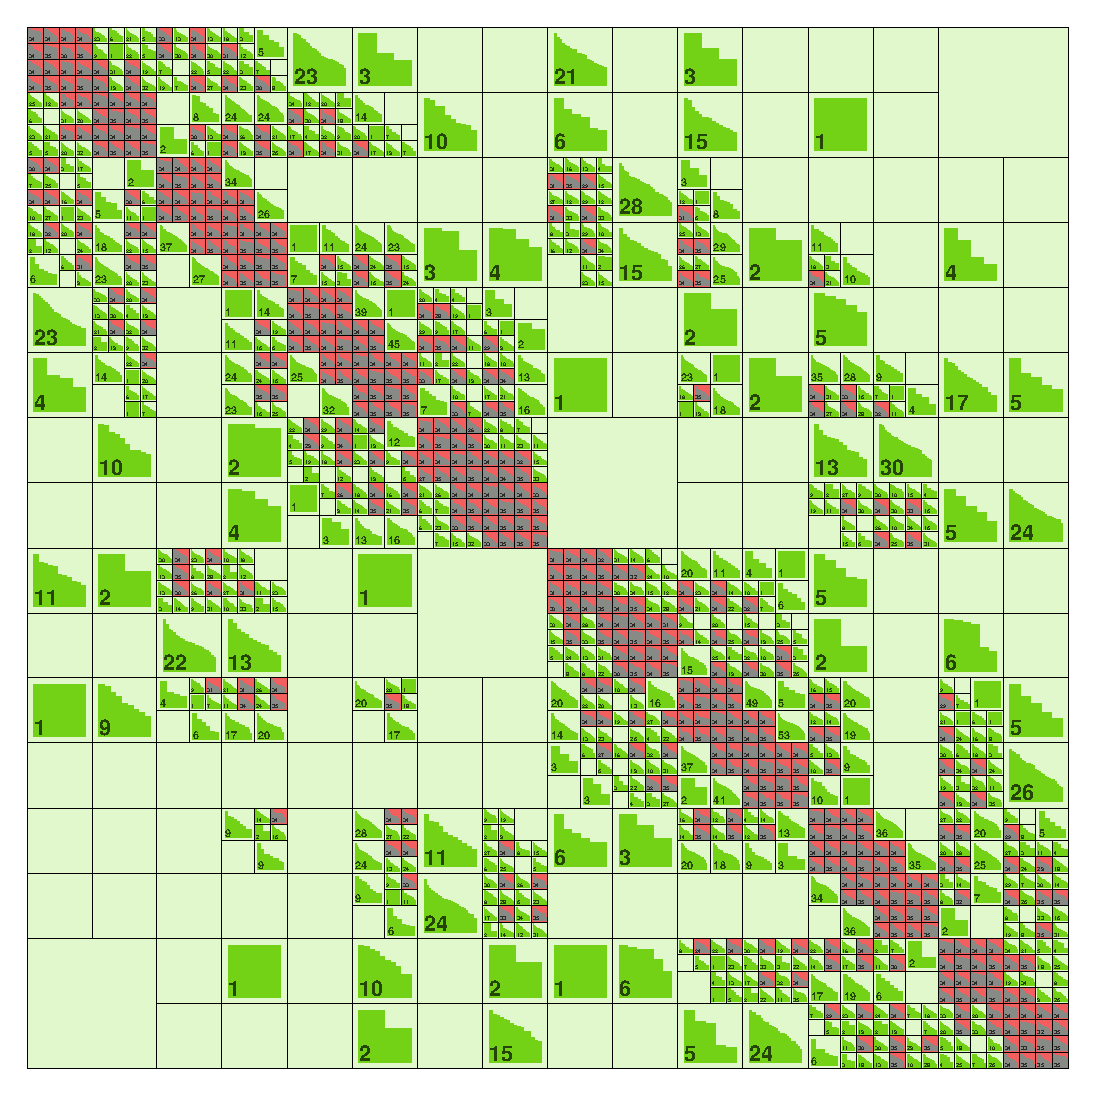
\includegraphics[width=0.85\textwidth]{extraplots/heat_inverse_problem_Hfull_hmatrix.eps}
    \end{column}
    \end{columns}

    \vspace{0.1in}
        \begin{itemize}
        \item We use H1 matrices in the numerical results via the
          HLIBpro software package, but any other H-matrix format
          could be used instead.
        \item Details in:
          \scriptsize
          \begin{itemize}
        \item W. Hackbusch, ``A sparse matrix arithmetic based on
          $\mathcal{H}$-matrices. Part I: Introduction to $\mathcal{H}$-matrices'', Computing,
          62 (1999), pp. 89-108.
        \item  R. Kriemann,
          ``HLIBpro user manual'', Max-Planck-Institute for
          Mathematics in the Sciences, Leipzig, 48 (2008).
          \end{itemize}
        \end{itemize}
        
\end{frame}
%---------------------------------------------------------------------
\begin{frame}
	\frametitle{Hierarchical matrix versus matrix free}
	\begin{itemize}
	\item Classical methods for building $\mathcal{H}$-matrix require matrix entries $\mathbf{H}_{ij}$
          \vspace{0.05in}
	\item New algebraic methods based on ``peeling process'' can build $\mathcal{H}$-matrix from matrix-vector products
          \vspace{0.05in}
	\item \textbf{Problem:} peeling process better than low rank, but \textbf{still expensive} (see for instance [*] below)
          \vspace{0.05in}
	\item Here we build the $\mathcal{H}$-matrix faster by taking advantage of the problem structure (details in [**])
	  \begin{itemize}
	  \item \textbf{Local sensitivities}
	  \item \textbf{Local mean-displacement invariance}
	  \item \textbf{Non-negative impulse responses}
	  \end{itemize}
	\end{itemize}

        \vspace{0.1in}
        \scriptsize
        \begin{itemize}
        \item [*] {T. Hartland, G. Stadler, M. Perego,
          K. Liegeois, N. Petra. ``Hierarchical off-diagonal low-rank
          approximation of Hessians in inverse problems, with application to
          ice sheet model initialization'', Inverse Problems, 39 (8), 2023. }
          \item [**] {Details in: N. Alger, T. Hartland, N. Petra,
            O. Ghattas. ``Point spread function approximation of high
            rank Hessians with locally supported non-negative integral
            kernels'', To appear in SIAM Journal on Scientific
            Computing (SISC).}
     \end{itemize}

\end{frame}
%---------------------------------------------------------------------------------%
\begin{frame}
  \frametitle{Fast high-rank Hessian approximation for Bayesian ice
    sheet inverse problems}
      \begin{itemize}
      \item {\bf Stage 1: Hessian approximation via product-convolution
        approximation:}
        %leads to fast access to matrix entries, which
        %makes
        %the approximation well-suited for hierarchical matrix compression.
        %to reduce the computational cost of the
        %{$\mathcal{H}$-matrice compression, we first approximate the Hessian
        %  using a {\note product-convolution approximation approach} that
        %  takes advantage of the Hessian's local translation invariance.
        \begin{itemize}
        \item Compute {\bf the impulse responses} of the Hessian operator at
          many points by applying the operator to a small number of Dirac
          combs of point sources.
          %\item Within each Dirac comb, the point sources must be spaced
          %  sufficiently far apart so that the impulse responses to those
          %  point sources do not overlap with each other or with the boundary.
        \item Estimate the required spacing of point sources by applying the
          operator to a small number of constant, linear, and quadratic
          functions.
        \item Once computed, the impulse responses are interpolated to approximate arbitrary Hessian entries.
        \end{itemize}
      \item {\bf Stage 2: $\mathcal{H}$-matrix compression:}
        \begin{itemize}
        \item Convert the product-convolution Hessian approximation to
          hierarchical matrix format.
        \item Invert the compressed matrix using fast hierarchical matrix
          arithmetic.
        \end{itemize}

        \item {\bf Stage 3: Hessian-approximation via
          $\mathcal{H}$-matrix compression:}
          \begin{itemize}
            \item Use this approximation to precondition linear systems involving the Hessian (e.g., solve the Newton system to
              compute the MAP point) and/or draw samples from the
              posterior.
          \end{itemize}
      \end{itemize}
\end{frame}


%-------------------------------------------------------------
\begin{frame}
  \frametitle{Stage1: Hessian approximation via PSF}
  \framesubtitle{Intuitively, one may think of
    impulse responses as ``columns'' of the integral kernel.}

  \begin{figure}
    \begin{center}
      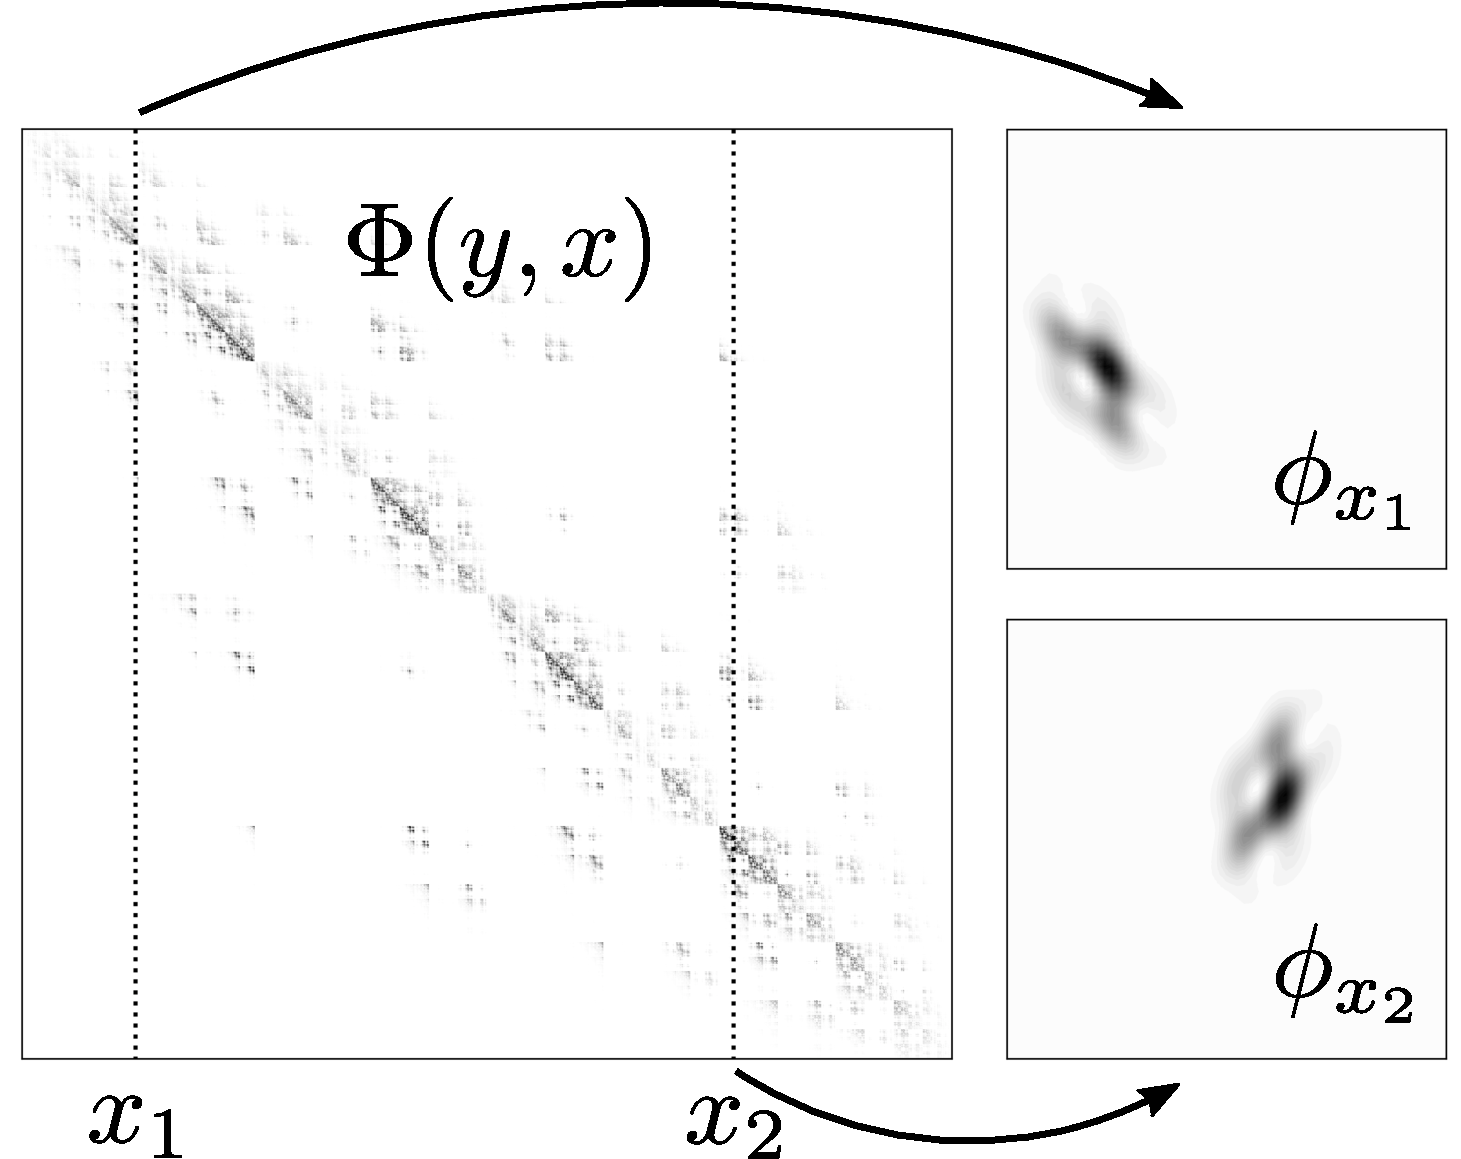
\includegraphics[scale=0.25]{localpsf_revised_figures/kernel_impulse_illustration2.pdf}
    \end{center}
    %\caption{Left: Matrix created by evaluating the integral
    %  kernel $\Phi$ for $\Aop$
    %  (Equation~\ref{eq:kernel_representation}) at all pairs of
    %  mesh vertices. This illustration is for the integral kernel
    %  given in Equation~\ref{eq:frog_kernel} in
    %  Section~\ref{sec:frog}. Dark colors indicate large entries
    %  and light colors indicate small entries. Rows and columns
    %  are ordered according to a kd-tree hierarchical
    %  clustering. Right: Impulse responses associated with points
    %  $x_1,x_2\in \Omega$, shown by the two dotted vertical
    %  lines. Intuitively, one may think of impulse responses as
    %  ``columns'' of the integral kernel.  }
    %\label{fig:frog_kernel_impulse_responses}
  \end{figure}

  \begin{center}
    Left: Integral kernel matrix. Right: Impulse responses associated
    with points $x_1,x_2\in \Omega$, shown by the two dotted vertical
    lines.
  \end{center}
\end{frame}
%-------------------------------------------------------------
\begin{frame}
  \frametitle{Stage1: Hessian approximation via PSF}

  \def \pos {0.5\columnwidth}
  \begin{figure}[ht]\centering
    \begin{tikzpicture}
      \only<1>{
        \node (1) at (0*\pos-0.4*\pos,  0*\pos){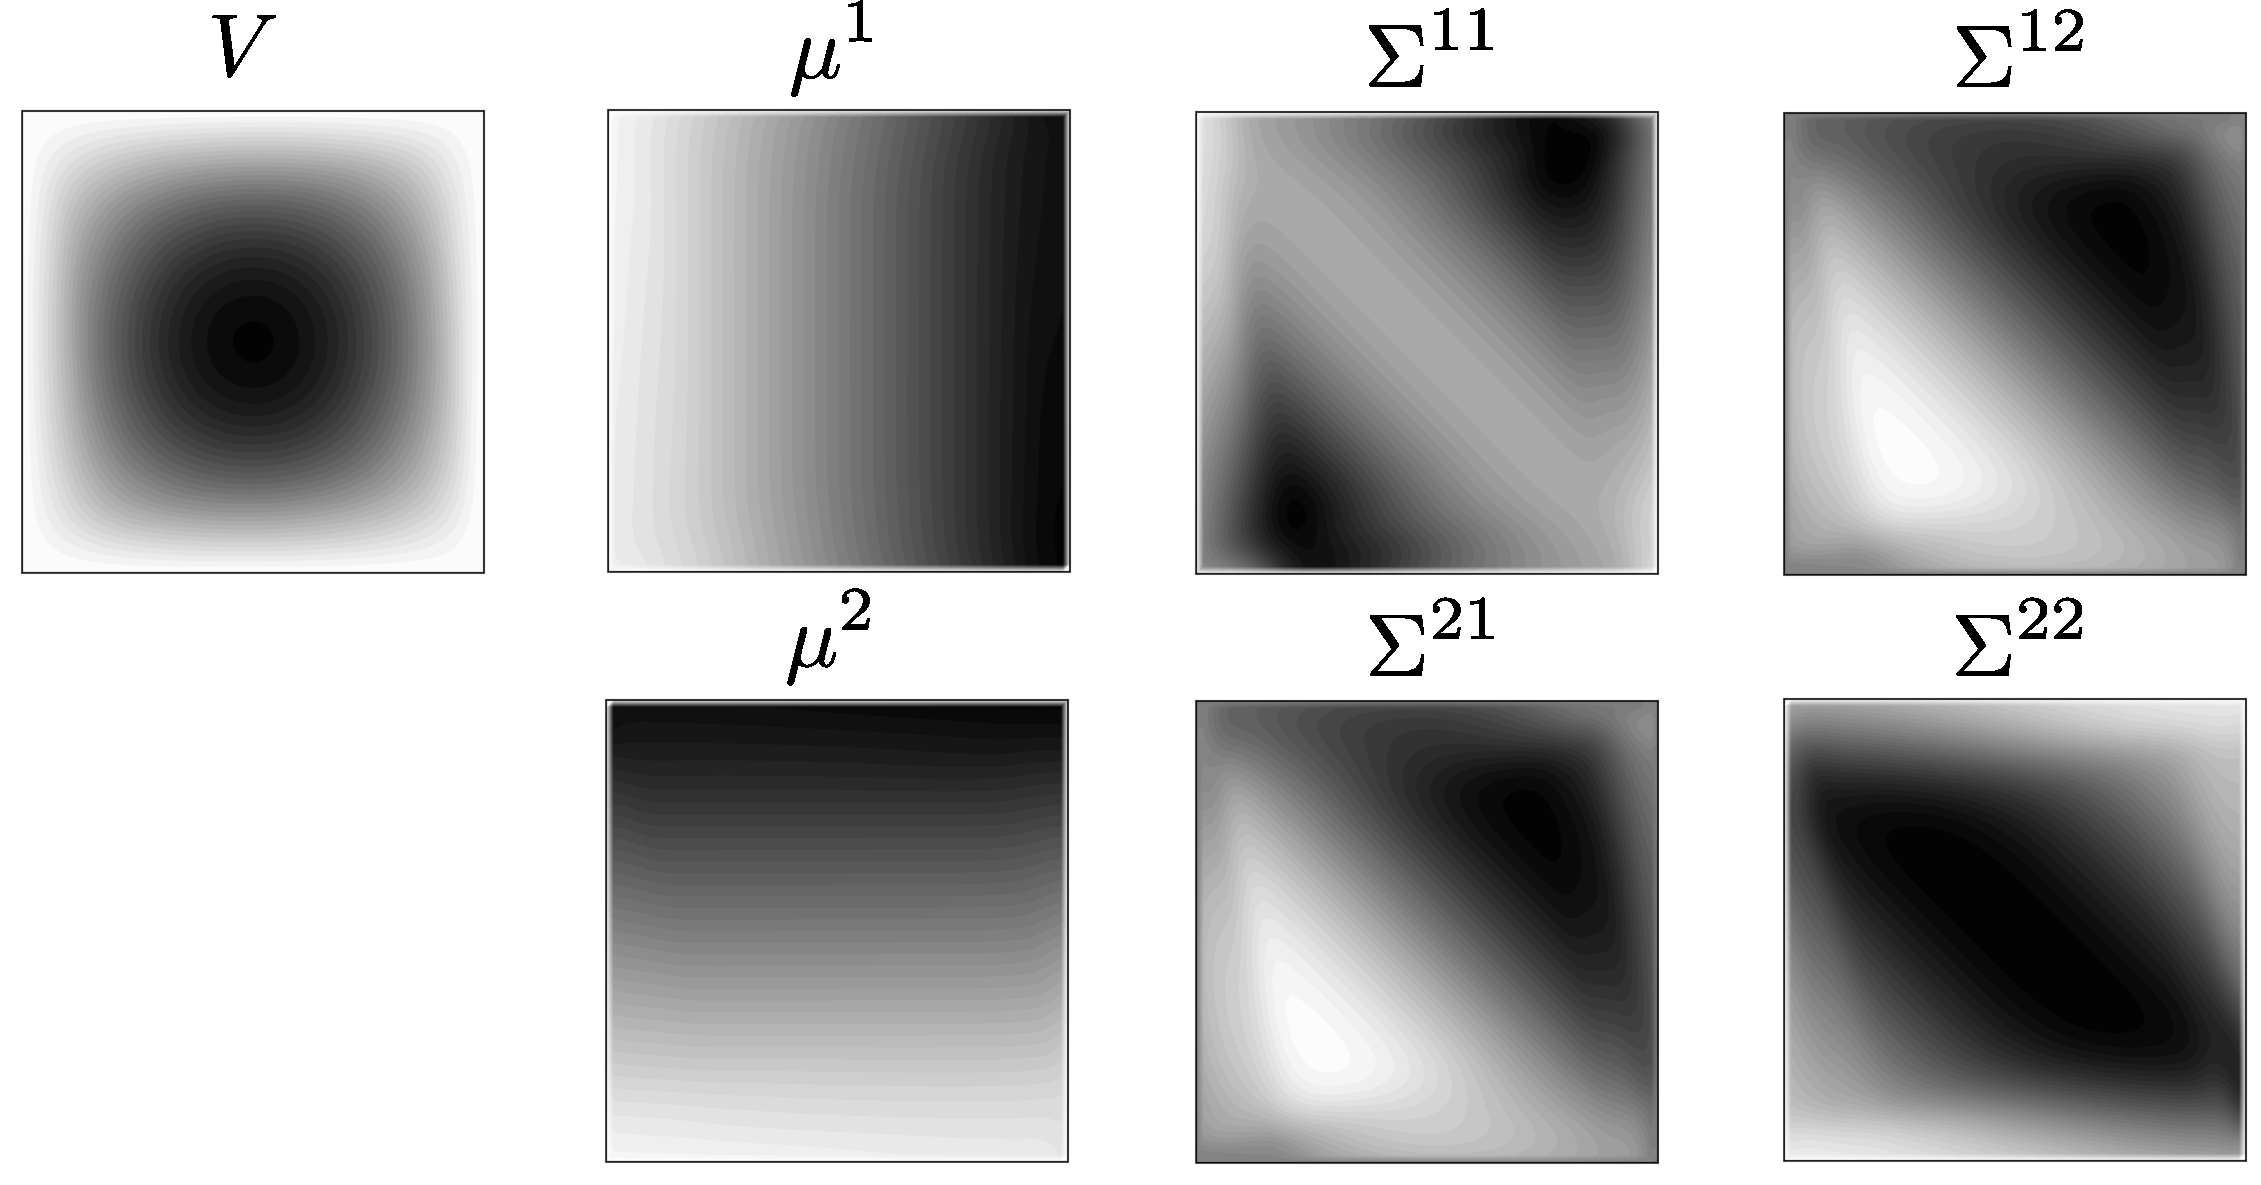
\includegraphics[scale=0.30]{localpsf_revised_figures/frog_moments3.pdf}};
      }
      \only<2>{
        \node (1) at (0*\pos-0.4*\pos,  0*\pos){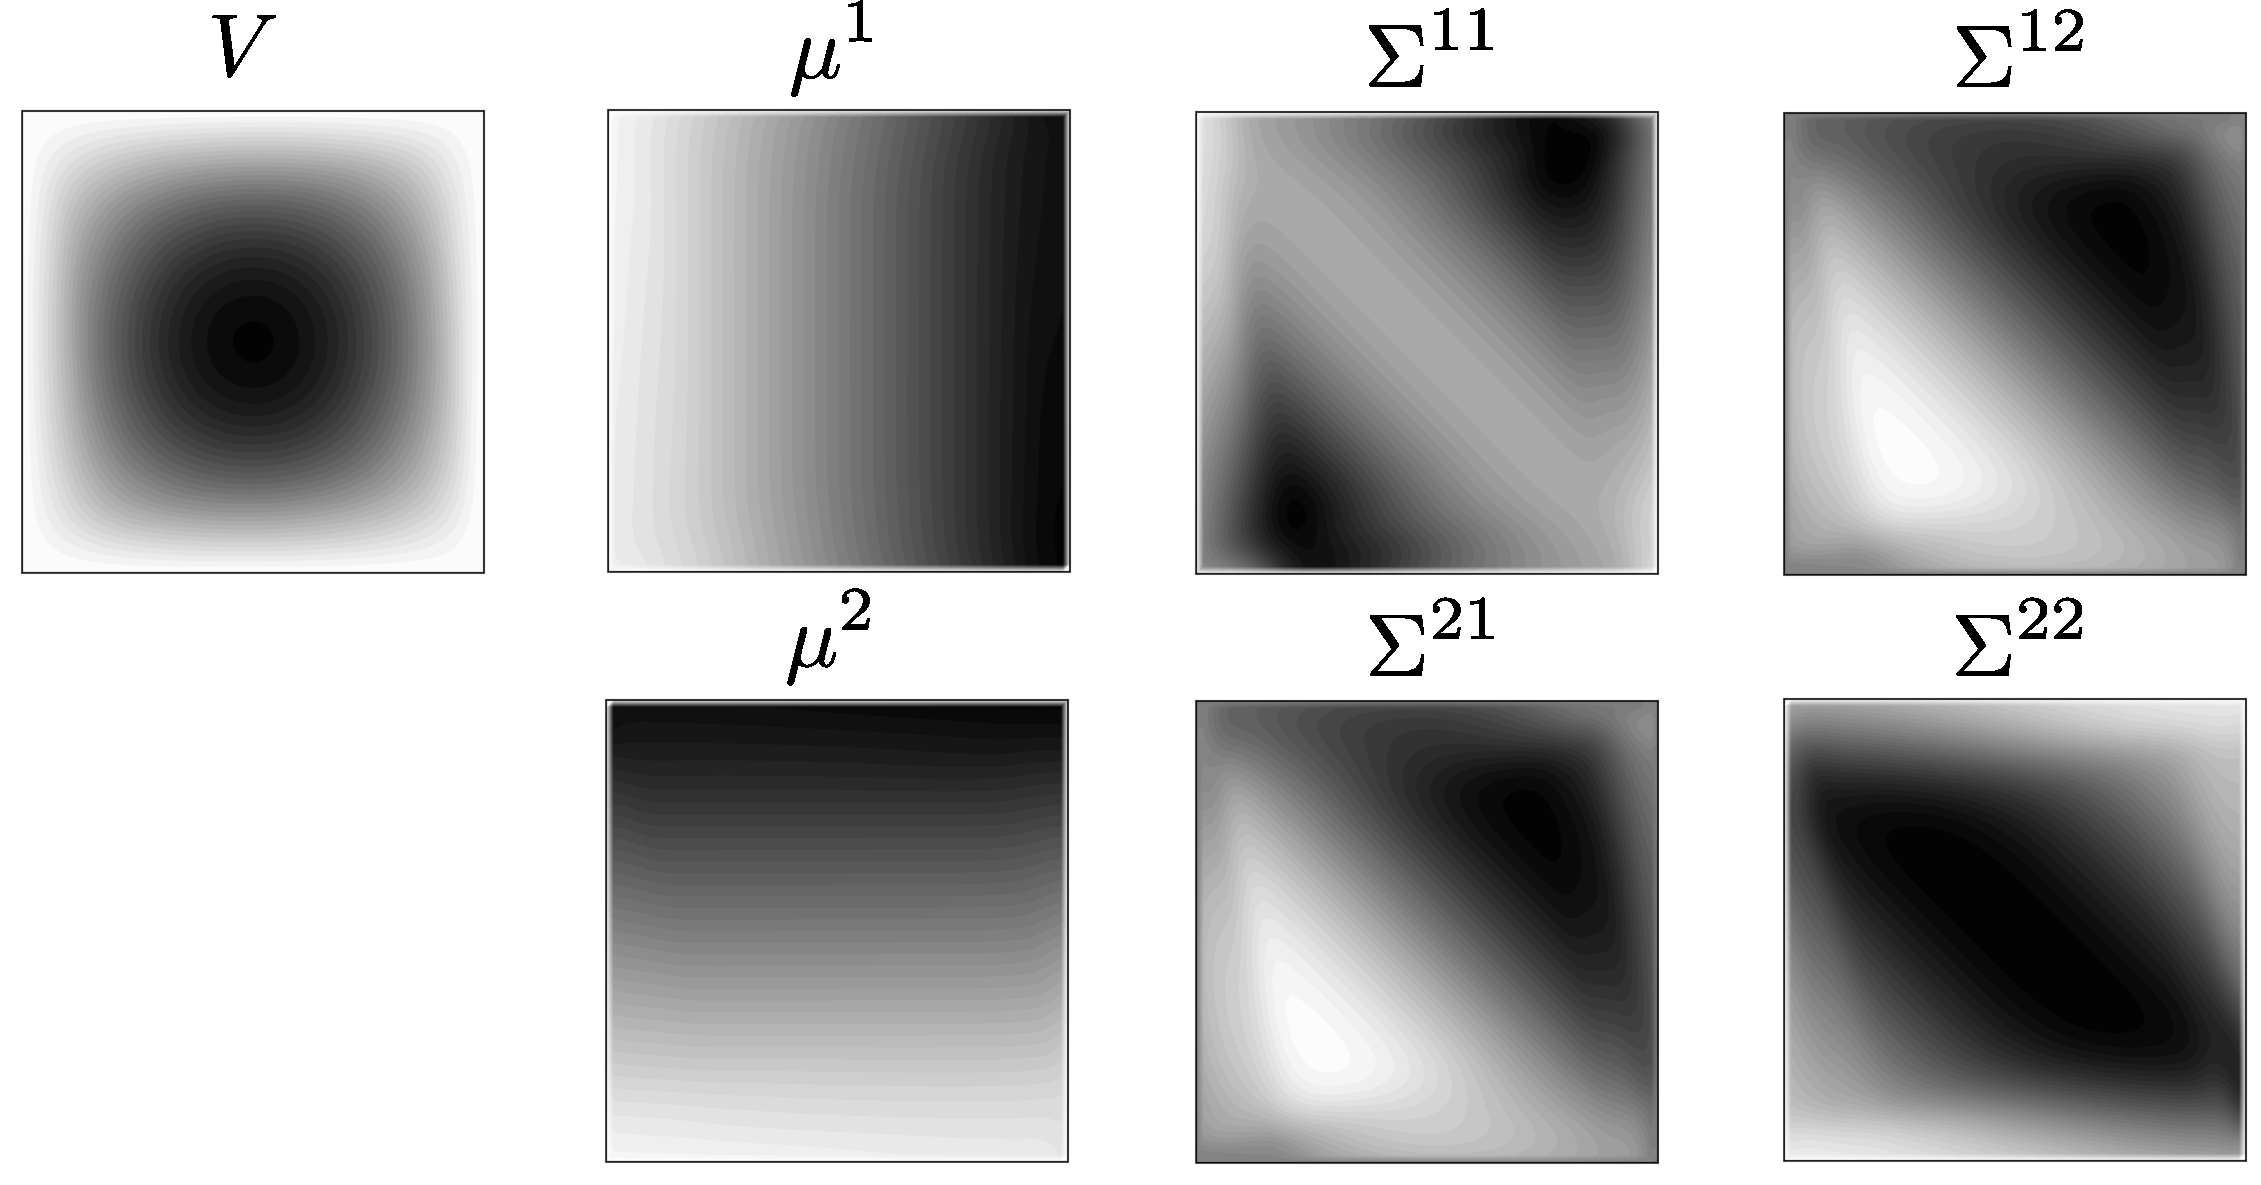
\includegraphics[scale=0.30]{localpsf_revised_figures/frog_moments3.pdf}};
        \node (2) at (0*\pos-1.1*\pos,  0*\pos-0.28*\pos){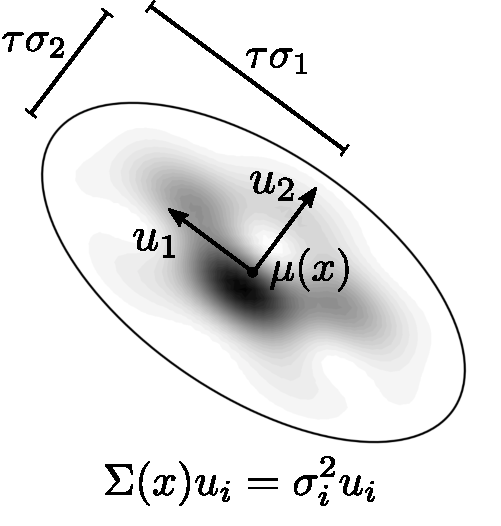
\includegraphics[scale=0.30]{localpsf_revised_figures/frog_ellipsoid_width2.pdf}};
      }
    %\begin{subfigure}[b]{0.34\textwidth}
      %\only<2>{\centering 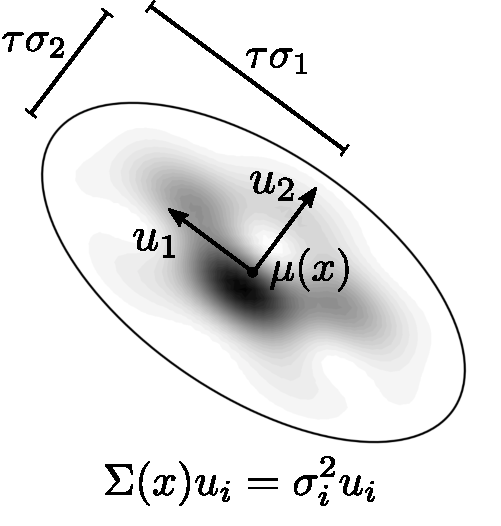
\includegraphics[scale=0.3]{localpsf_revised_figures/frog_ellipsoid_width2.pdf}}
    %\end{subfigure}
    %\caption{Left: Impulse response moments: scaling factor
    %  ($V$), mean ($\mu$), and covariance ($\Sigma$). For each
    %  point $x \in \Omega$, the quantity $V(x)$ is the integral
    %  of $\phi_x$ over $\Omega$, $\mu(x)$ is the location that
    %  $\phi_x$ is centered at, and $\Sigma(x)$ is a matrix with
    %  eigenvectors and eigenvalues that characterize the width of
    %  $\phi_x$ (see Section~\ref{sec:intromoments}). Right:
    %  Ellipsoid support for an impulse response.  This ellipsoid
    %  is the set of points within $\tau$ standard deviations of
    %  the mean of the Gaussian distribution with mean
    %  $\spatialmean(x)$ and covariance $\spatialcov(x)$. The
    %  scaling factor $V(x)$ characterizes the magnitude of
      %  $\phi_x$.  } \label{fig:frog_moments_ellipsoid}
      \end{tikzpicture}
  \end{figure}

  \begin{center}
    \only<1> {Impulse response moments: scaling factor ($V$), mean
    ($\mu$), and covariance ($\Sigma$).}
    \only<2> {Impulse response moments: scaling factor ($V$), mean
    ($\mu$), and covariance ($\Sigma$). Bottom left: Ellipsoid support
    for an impulse response.}
  \end{center}
\end{frame}
  %-------------------------------------------------------------
\begin{frame}
  \frametitle{Stage1: Hessian approximation via PSF}
  \framesubtitle{Illustration of the process to compute one impulse
    response batch}
\begin{figure}
	\centering 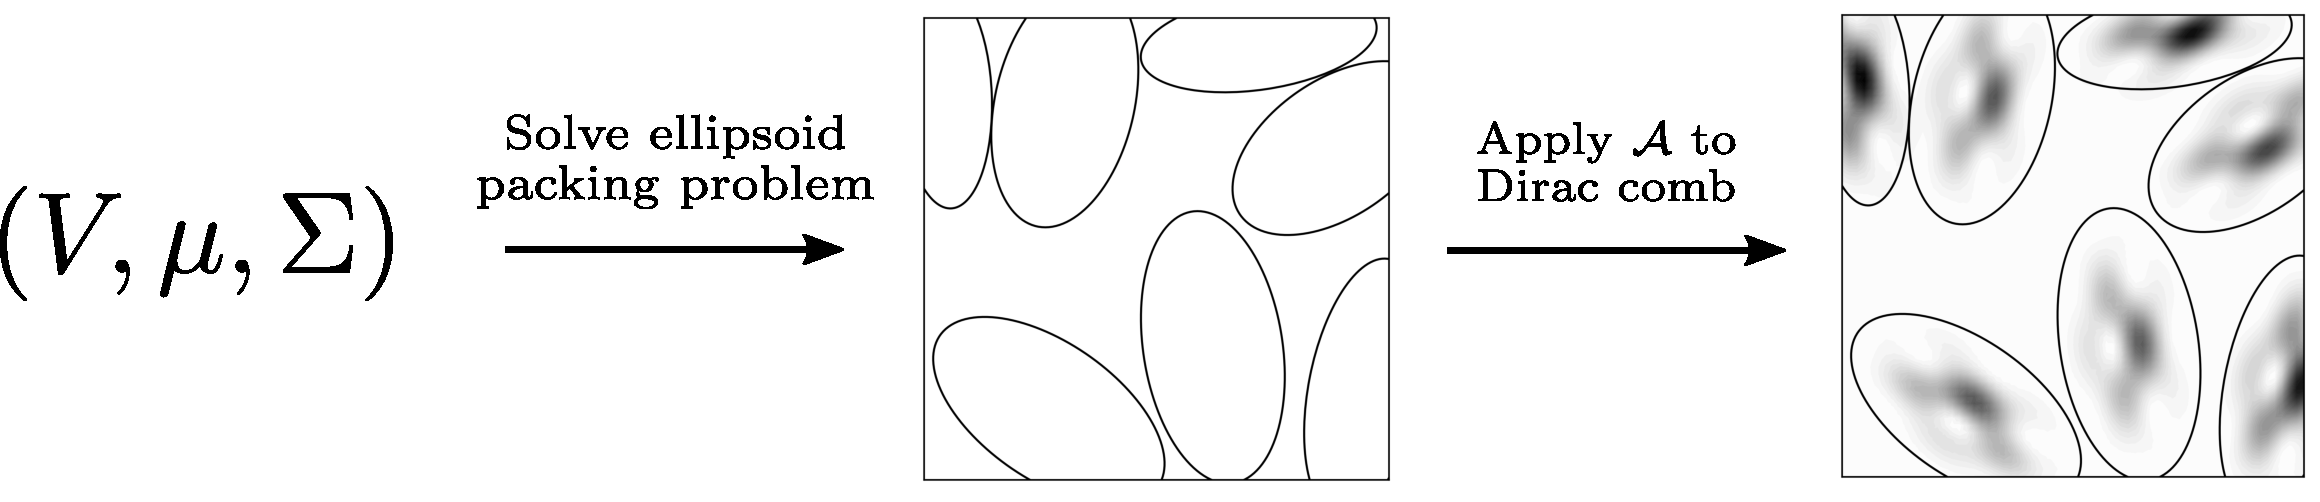
\includegraphics[scale=0.3]{localpsf_revised_figures/frog_batches3.pdf}
	%\caption{Illustration of the process to compute one impulse
        %  response batch. Impulse response moments are first used to
        %  form ellipsoid shaped estimates of the supports of impulse
        %  responses (Equation~\ref{eq:support_ellipsoid}). Then, an
        %  ellipsoid packing problem is solved to choose batches of
        %  non-overlapping support ellipsoids
        %  (Section~\ref{sec:sample_point_selection}).  Finally,
        %  $\Aop$ is applied to a Dirac comb associated with the
        %  points $x_i$, which correspond to the ellipsoids
        %  (Section~\ref{sec:get_impulse_response}). The process is
        %  repeated to form more batches.}
	%\label{fig:frog_batches}
\end{figure}

\begin{enumerate}
\item Impulse response moments are first used to form ellipsoid shaped
  estimates of the supports of impulse responses
\item Then, an ellipsoid
  packing problem is solved to choose batches of non-overlapping
  support ellipsoids.
\item Finally,  $\Aop$ is applied to a Dirac comb associated with the
  points $x_i$, which correspond to the ellipsoids
\item  The process is
  repeated to form more batches.
\end{enumerate}

\end{frame}
%-------------------------------------------------------------
\begin{frame}
  \frametitle{Stage1: Hessian approximation via PSF}
\framesubtitle{Kernel entry approximation via radial basis function interpolation}
\begin{figure}
	\centering 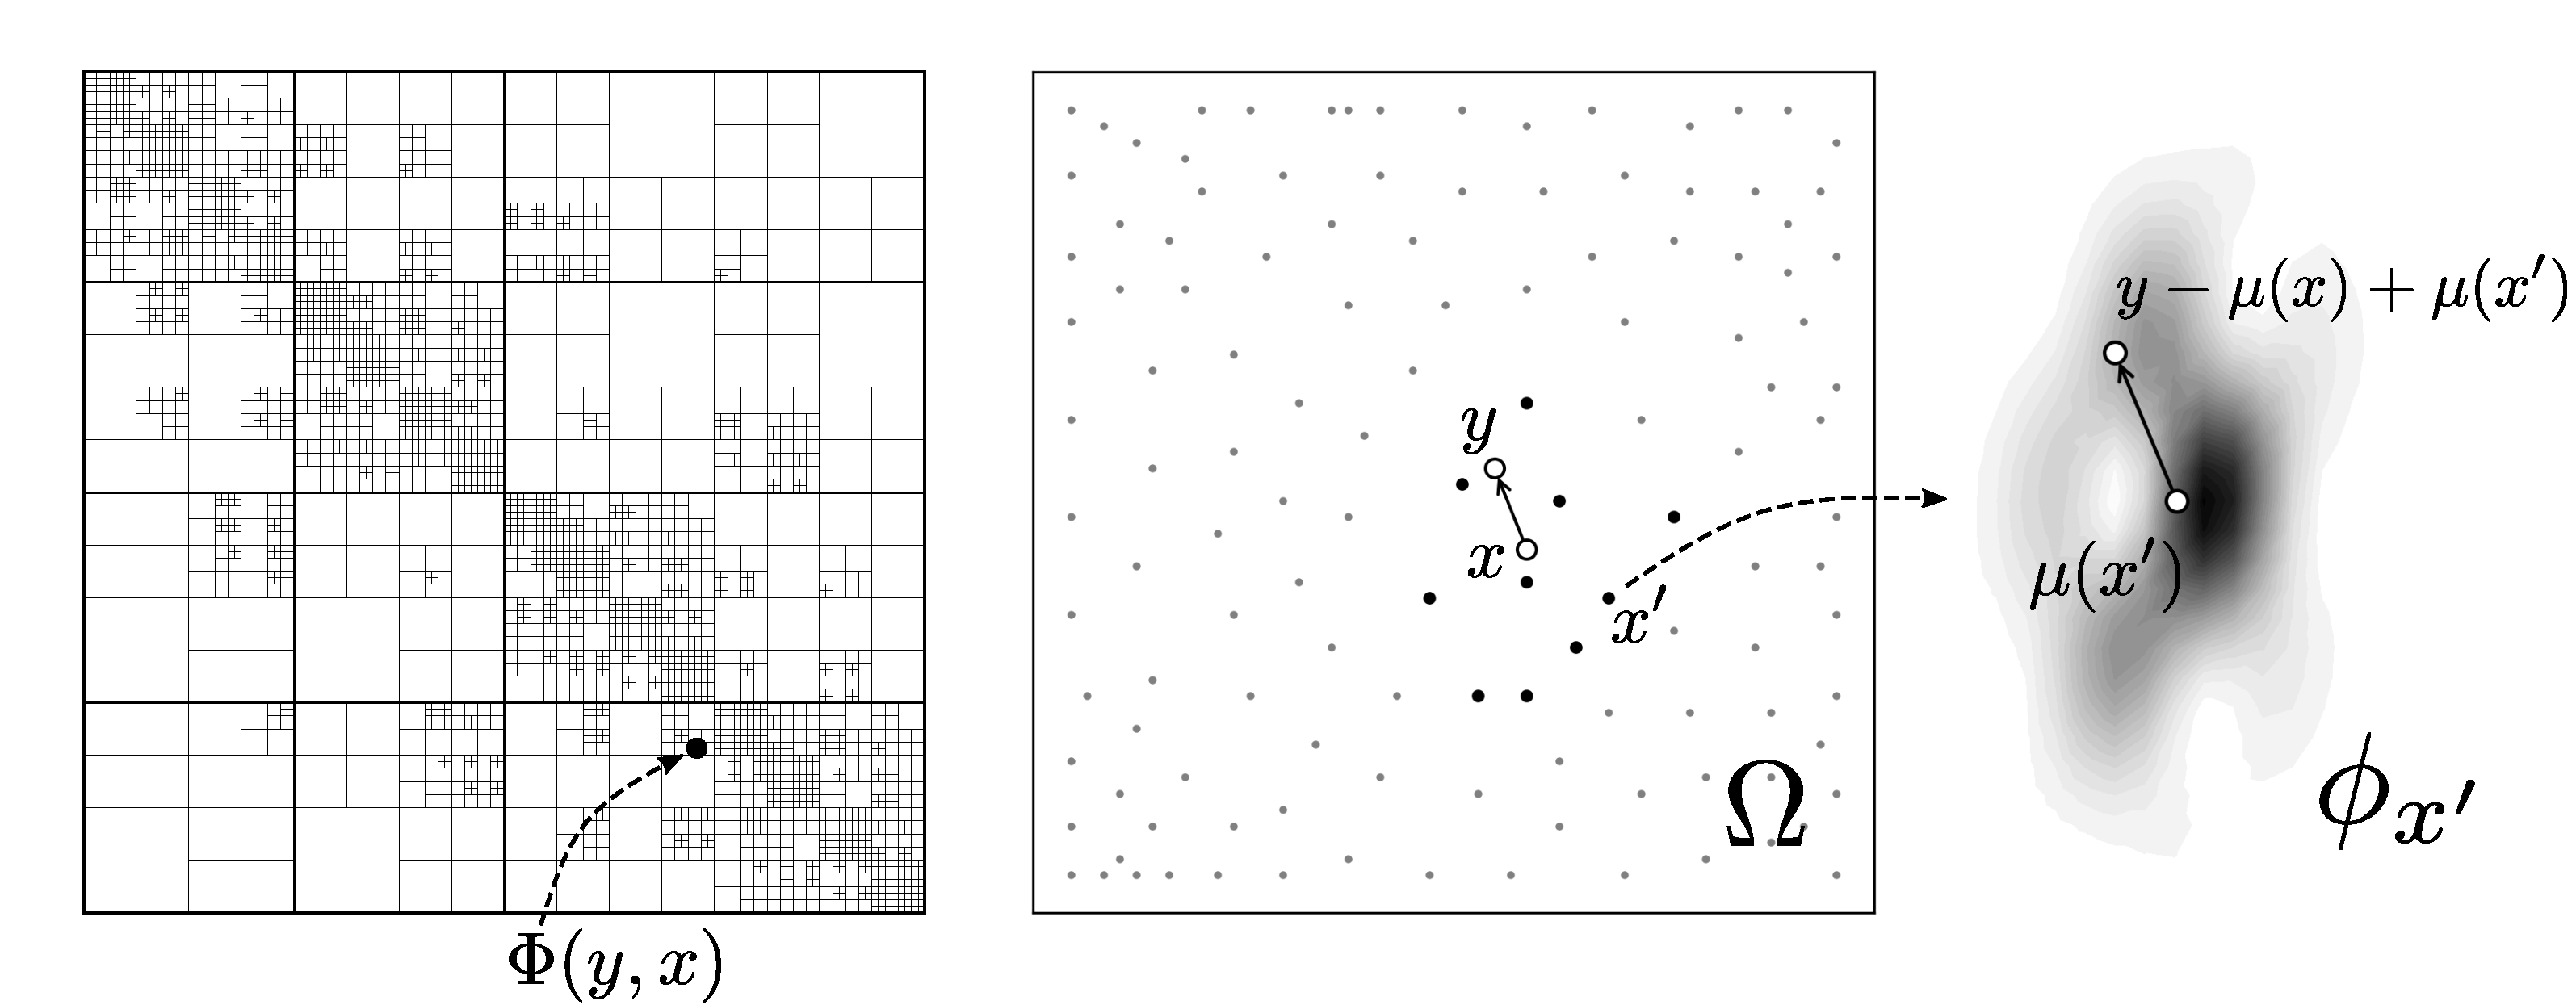
\includegraphics[scale=0.2]{localpsf_revised_figures/frog_hmatrix_knn_impulse3.pdf}
	%\caption{Left: H-matrix structure for $\Aker$. Computing an
        %  entry of this matrix requires evaluating the integral
        %  kernel, $\Phi(y,x)$, at a pair of points $(y,x) \in \Omega
        %  \times \Omega$.  Center: Kernel evaluation points $x$ and
        %  $y$ (black circles), sample points for the approximation
        %  (light gray and black dots), and the $k_n$ sample points,
        %  $x'$, that are nearest to $x$ (black dots). Right: Known
        %  impulse response at $x'$. Using radial basis function
        %  interpolation, the desired kernel entry is approximated as
        %  a weighted linear combination of translated and scaled
        %  versions of impulse responses at the points $x'$
        %  (Section~\ref{sec:approximate_kernel_entries}).
        %  } \label{fig:hmatrix_neighbors_frog}
\end{figure}

\begin{center}
  Left: H-matrix structure for $\Aker$. Center: Kernel evaluation
  points $x$ and $y$ (black circles), sample points for the
  approximation (light gray and black dots), and the $k_n$ sample
  points, $x'$, that are nearest to $x$ (black dots). Right: Known
  impulse response at $x'$.
\end{center}

%\begin{center}
%  Using radial basis function interpolation, the desired kernel entry
%  is approximated as a weighted linear combination of translated and
%  scaled versions of impulse responses at the points $x'$
%\end{center}
\end{frame}

%---------------------------------------------------------------------
\begin{frame}
  \frametitle{Stage1: Hessian approximation via PSF}
  \framesubtitle{Quality of the approximation}
  
  \begin{figure}
    \centering
    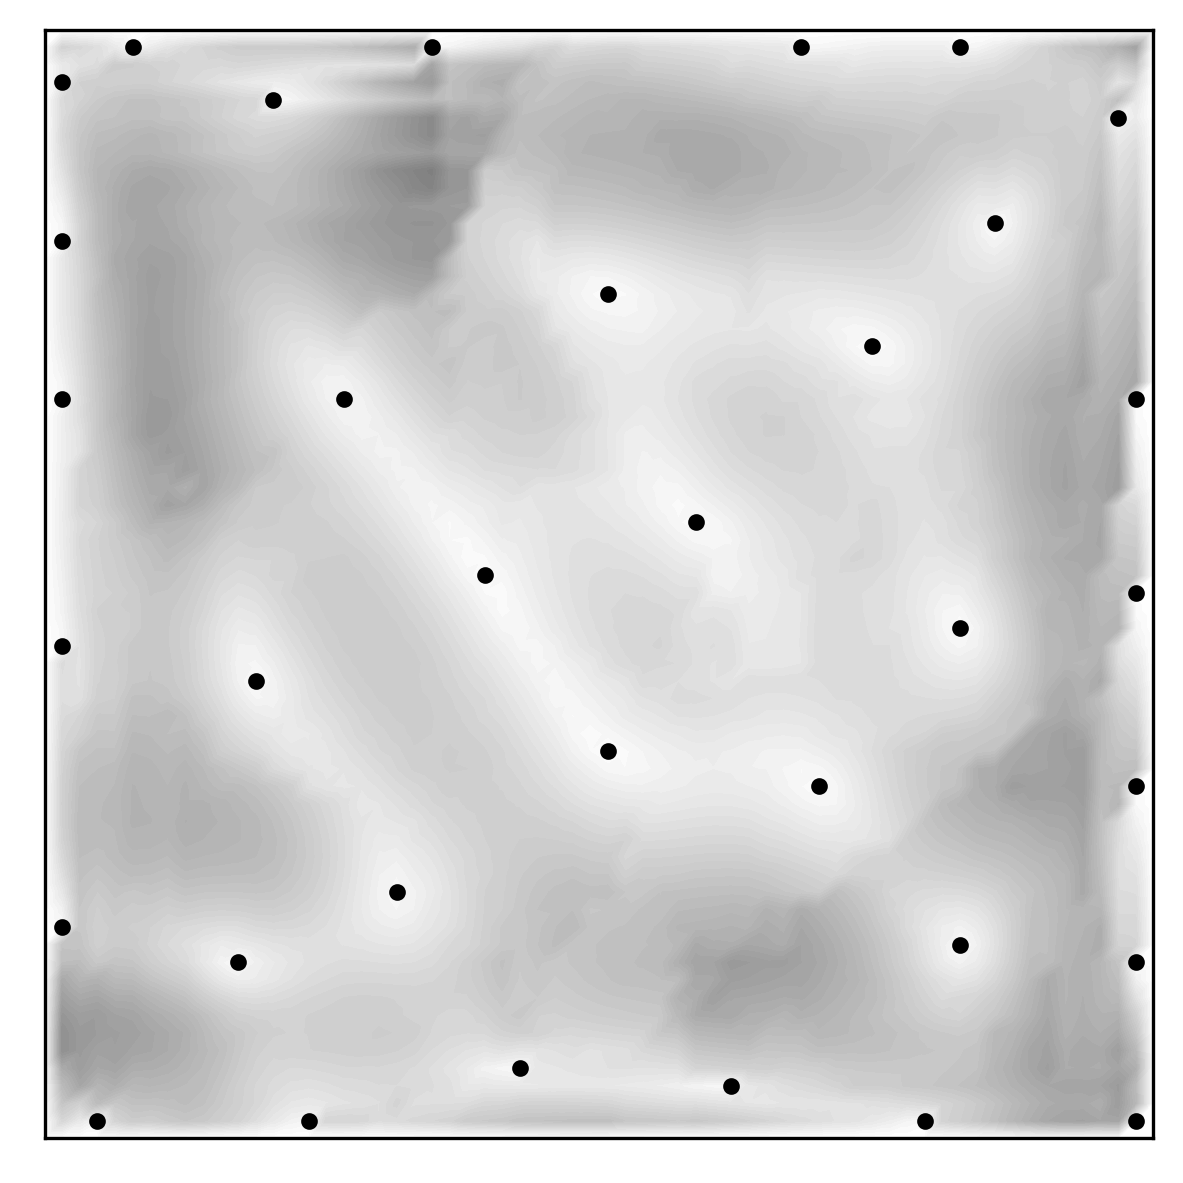
\includegraphics[scale=0.35]{localpsf_revised_figures/frog_column_errors_psf5.png}
    \hfill
    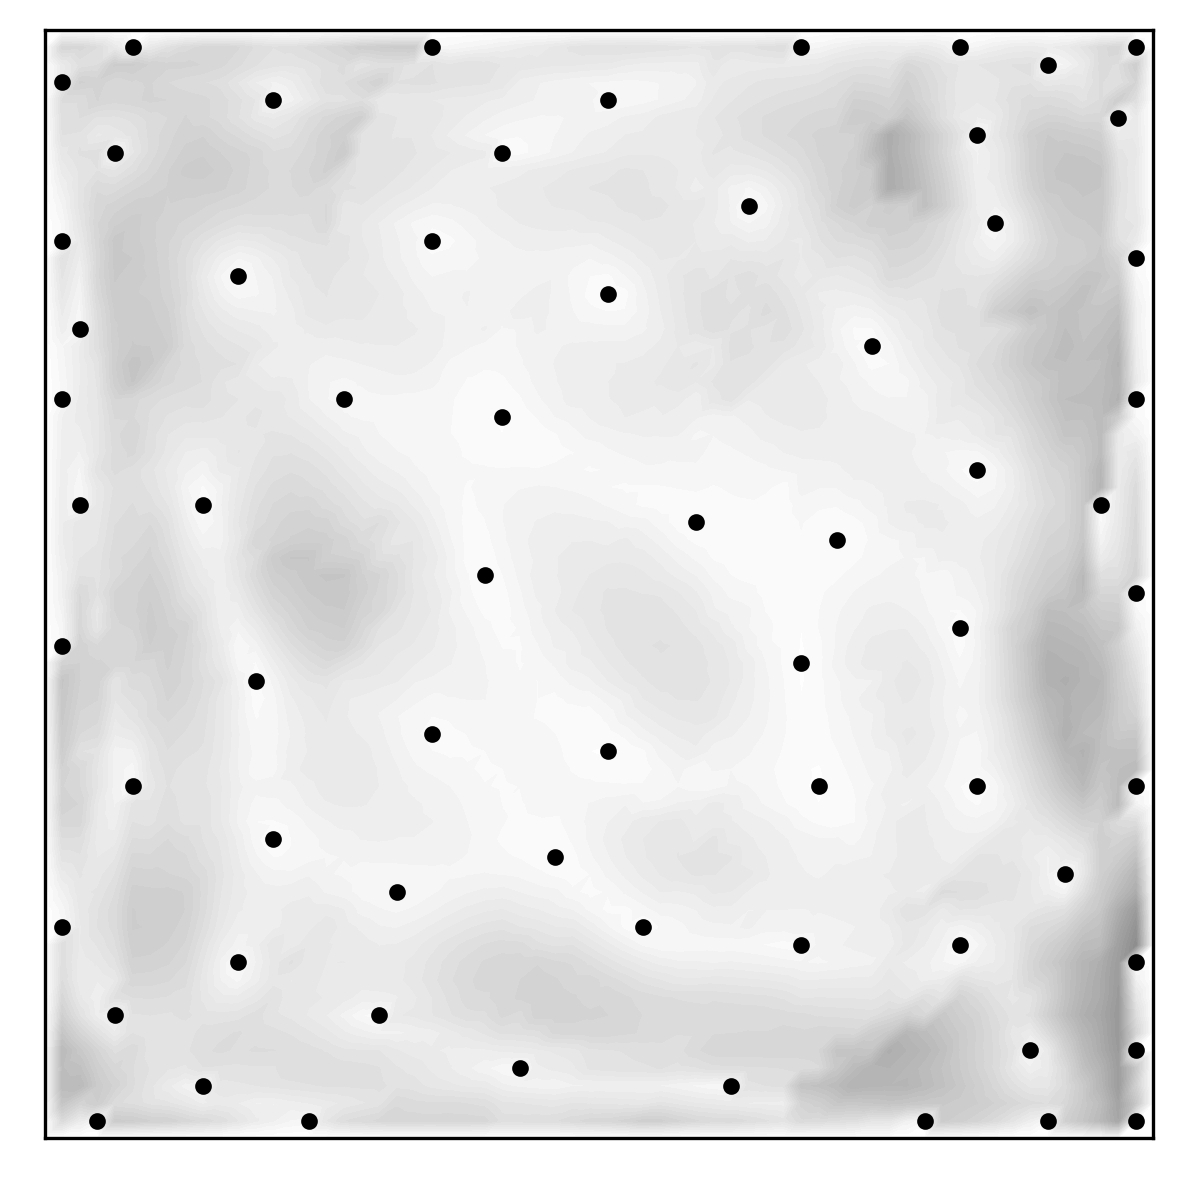
\includegraphics[scale=0.35]{localpsf_revised_figures/frog_column_errors_psf10.png}
    \hfill
    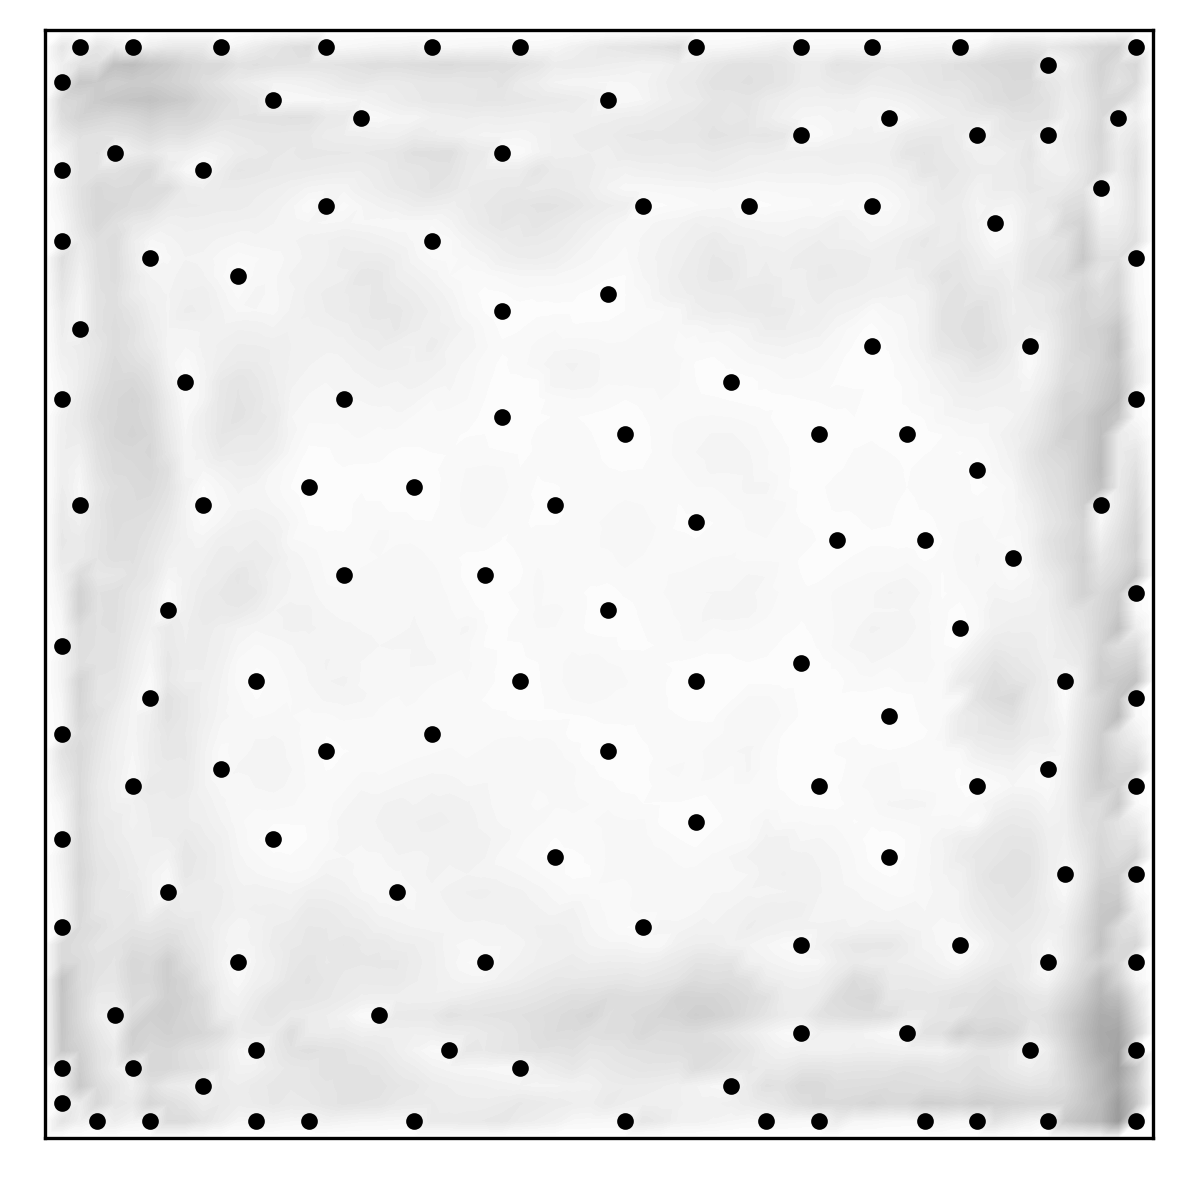
\includegraphics[scale=0.35]{localpsf_revised_figures/frog_column_errors_psf20.png}
    \hfill
    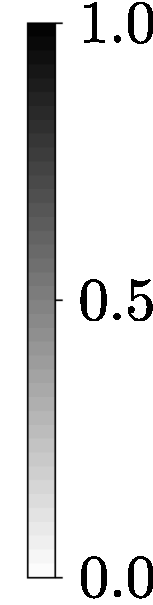
\includegraphics[scale=0.35]{localpsf_revised_figures/frog_colorbar_edited1.pdf}
    %\caption{Relative error, $||\Phi(\cdot,x) -
    %  \widetilde{\Phi}(\cdot,x)||/||\Phi(\cdot,x)||$, in the
    %  approximation of the ``column'' of the integral kernel
    %  associated with $x$, using 5 (left), 10 (center) and 20
    %  (right) impulse response batches. Sample points are
    %  indicated by black dots. The error associated with the point
    %  $x$ is the shade of the image at location $x$, with white
    %  indicating zero error and black indicating $100\%$ error. At
    %  the sample points, the error is zero. The further the point
    %  $x$ is from the samples points, the larger the error. Adding
    %  more batches yields a more accurate approximation.  }
  \end{figure}

  \begin{center}
    Relative error, $||\Phi(\cdot,x) -
      \widetilde{\Phi}(\cdot,x)||/||\Phi(\cdot,x)||$, in the
      approximation of the ``column'' of the integral kernel
      associated with $x$, using 5 (left), 10 (center) and 20
      (right) impulse response batches.
  \end{center}
\end{frame}
%--------------------------------------------------------------------------
\begin{frame}
  \frametitle{Ellipsoid estimates for the supports
    of impulse responses} \framesubtitle{Blur kernel (left two
    columns) and a Ricker wavelet-type kernel (right two columns)}
  \begin{figure}
    \centering
	{
	  \begin{tabular}{cccc}
	    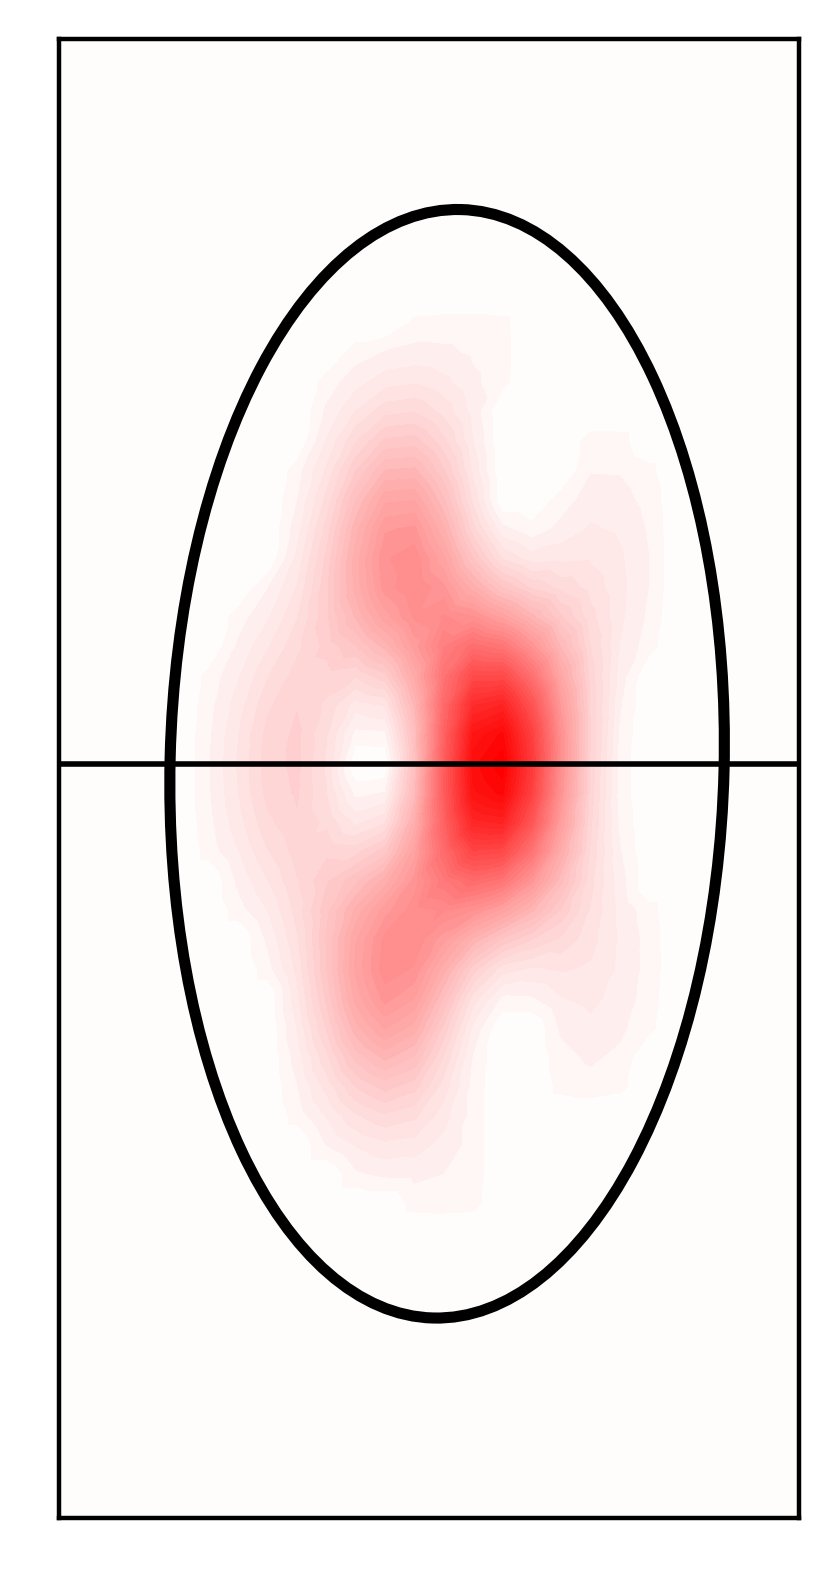
\includegraphics[scale=0.2]{localpsf_revised_figures/frog_ellipsoid_a=1.0.png} & 
	    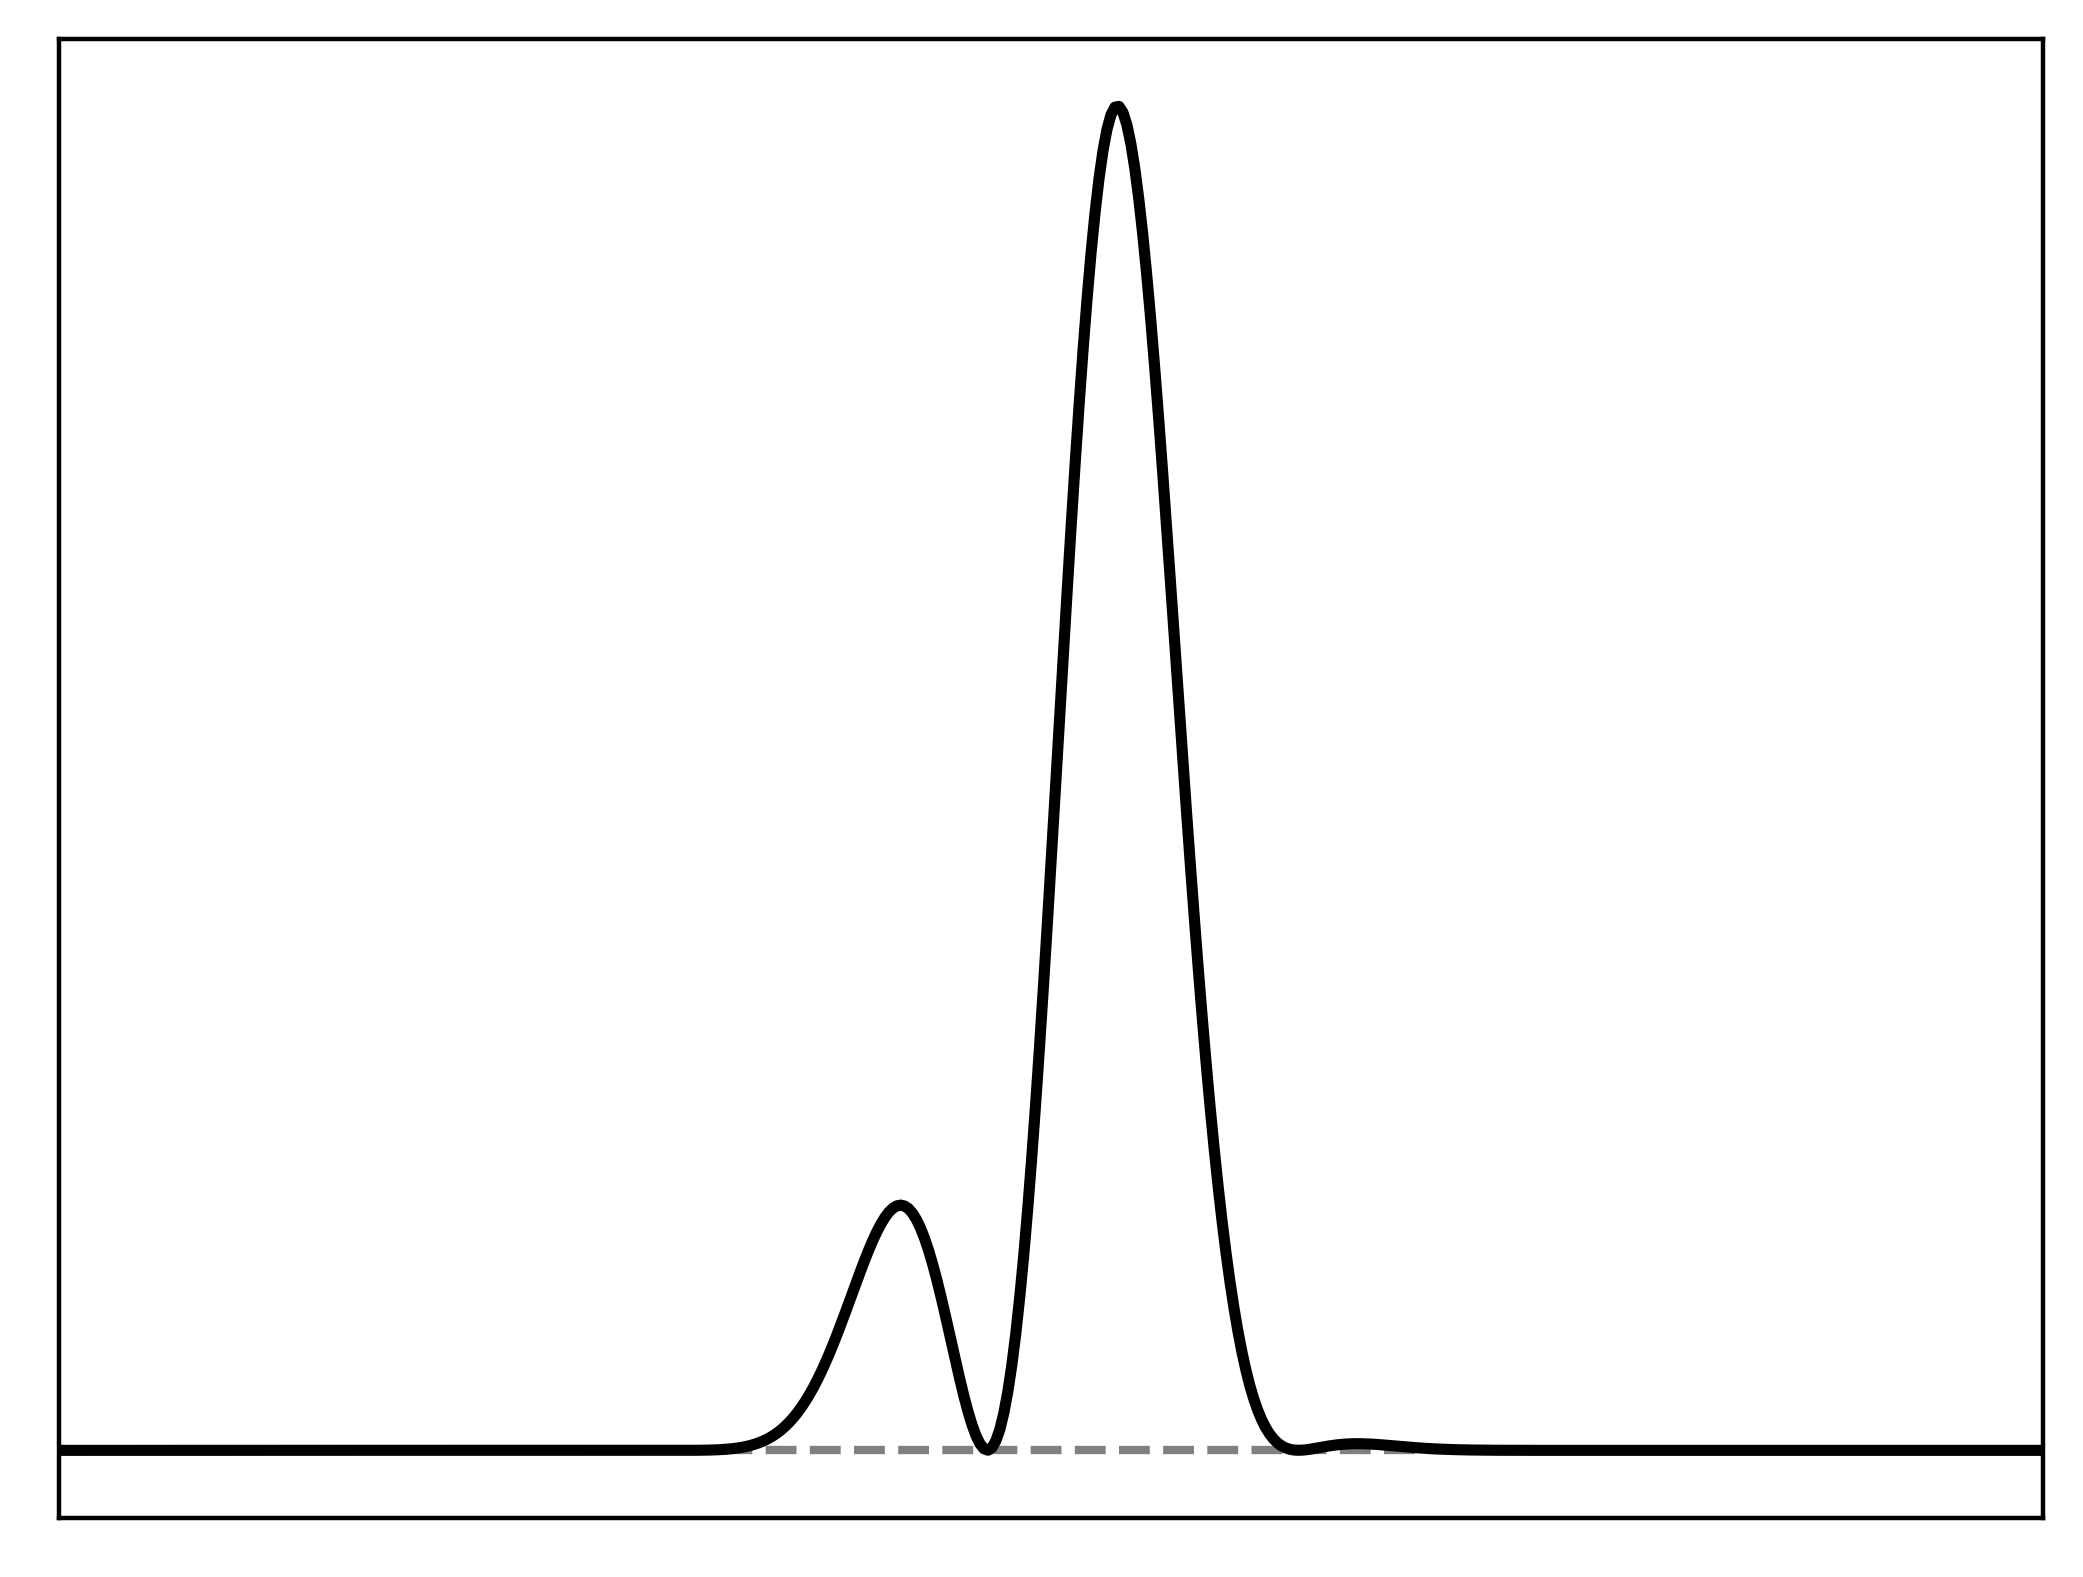
\includegraphics[scale=0.2]{localpsf_revised_figures/frog_1d_a=1.0.png} & 
	    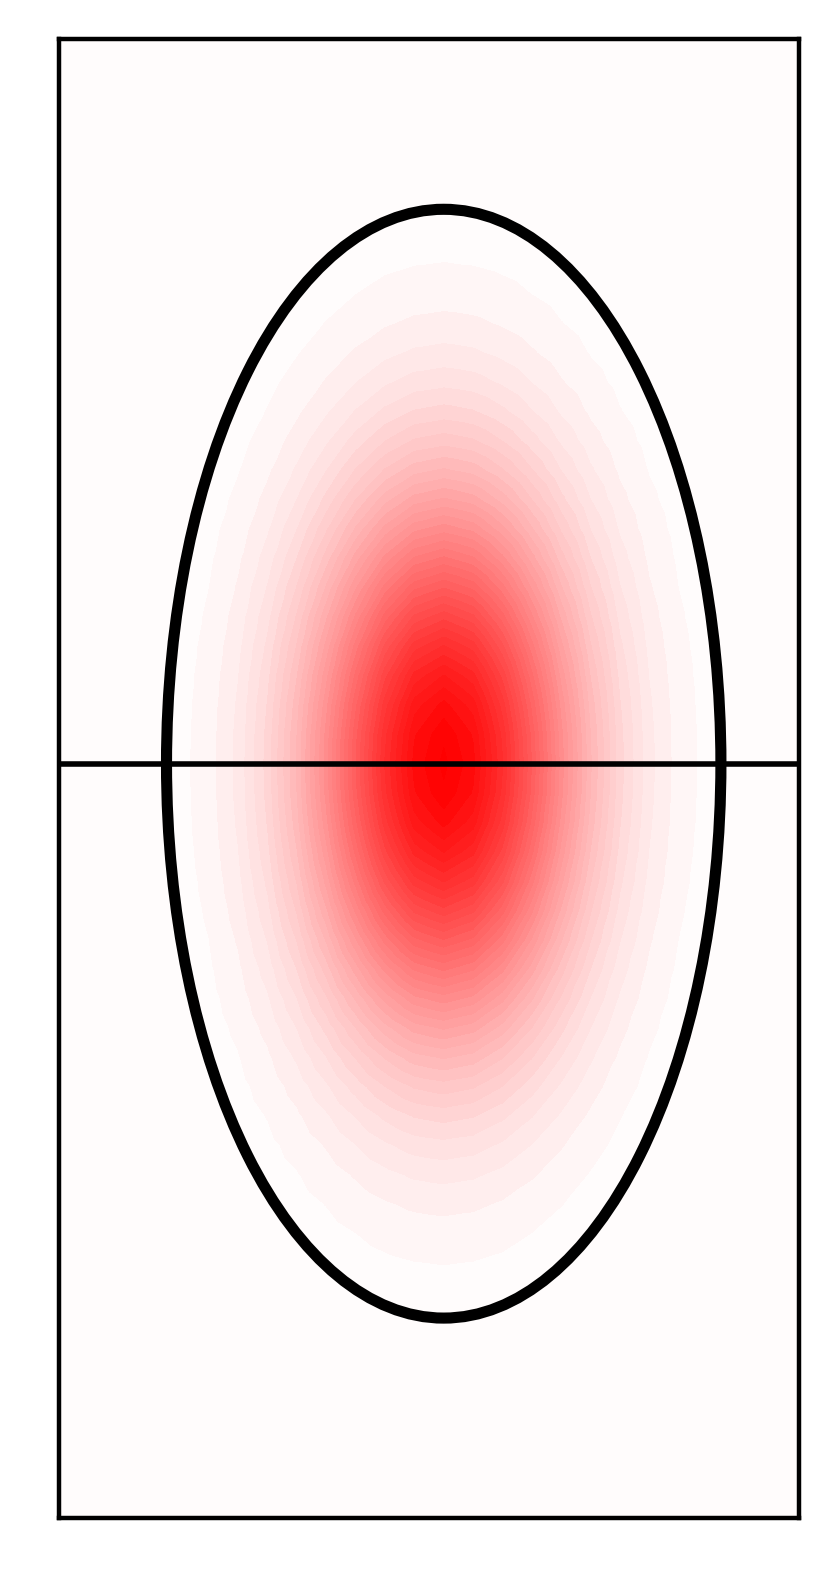
\includegraphics[scale=0.2]{localpsf_revised_figures/ricker_ellipsoid_a=0.0.png} & 
	    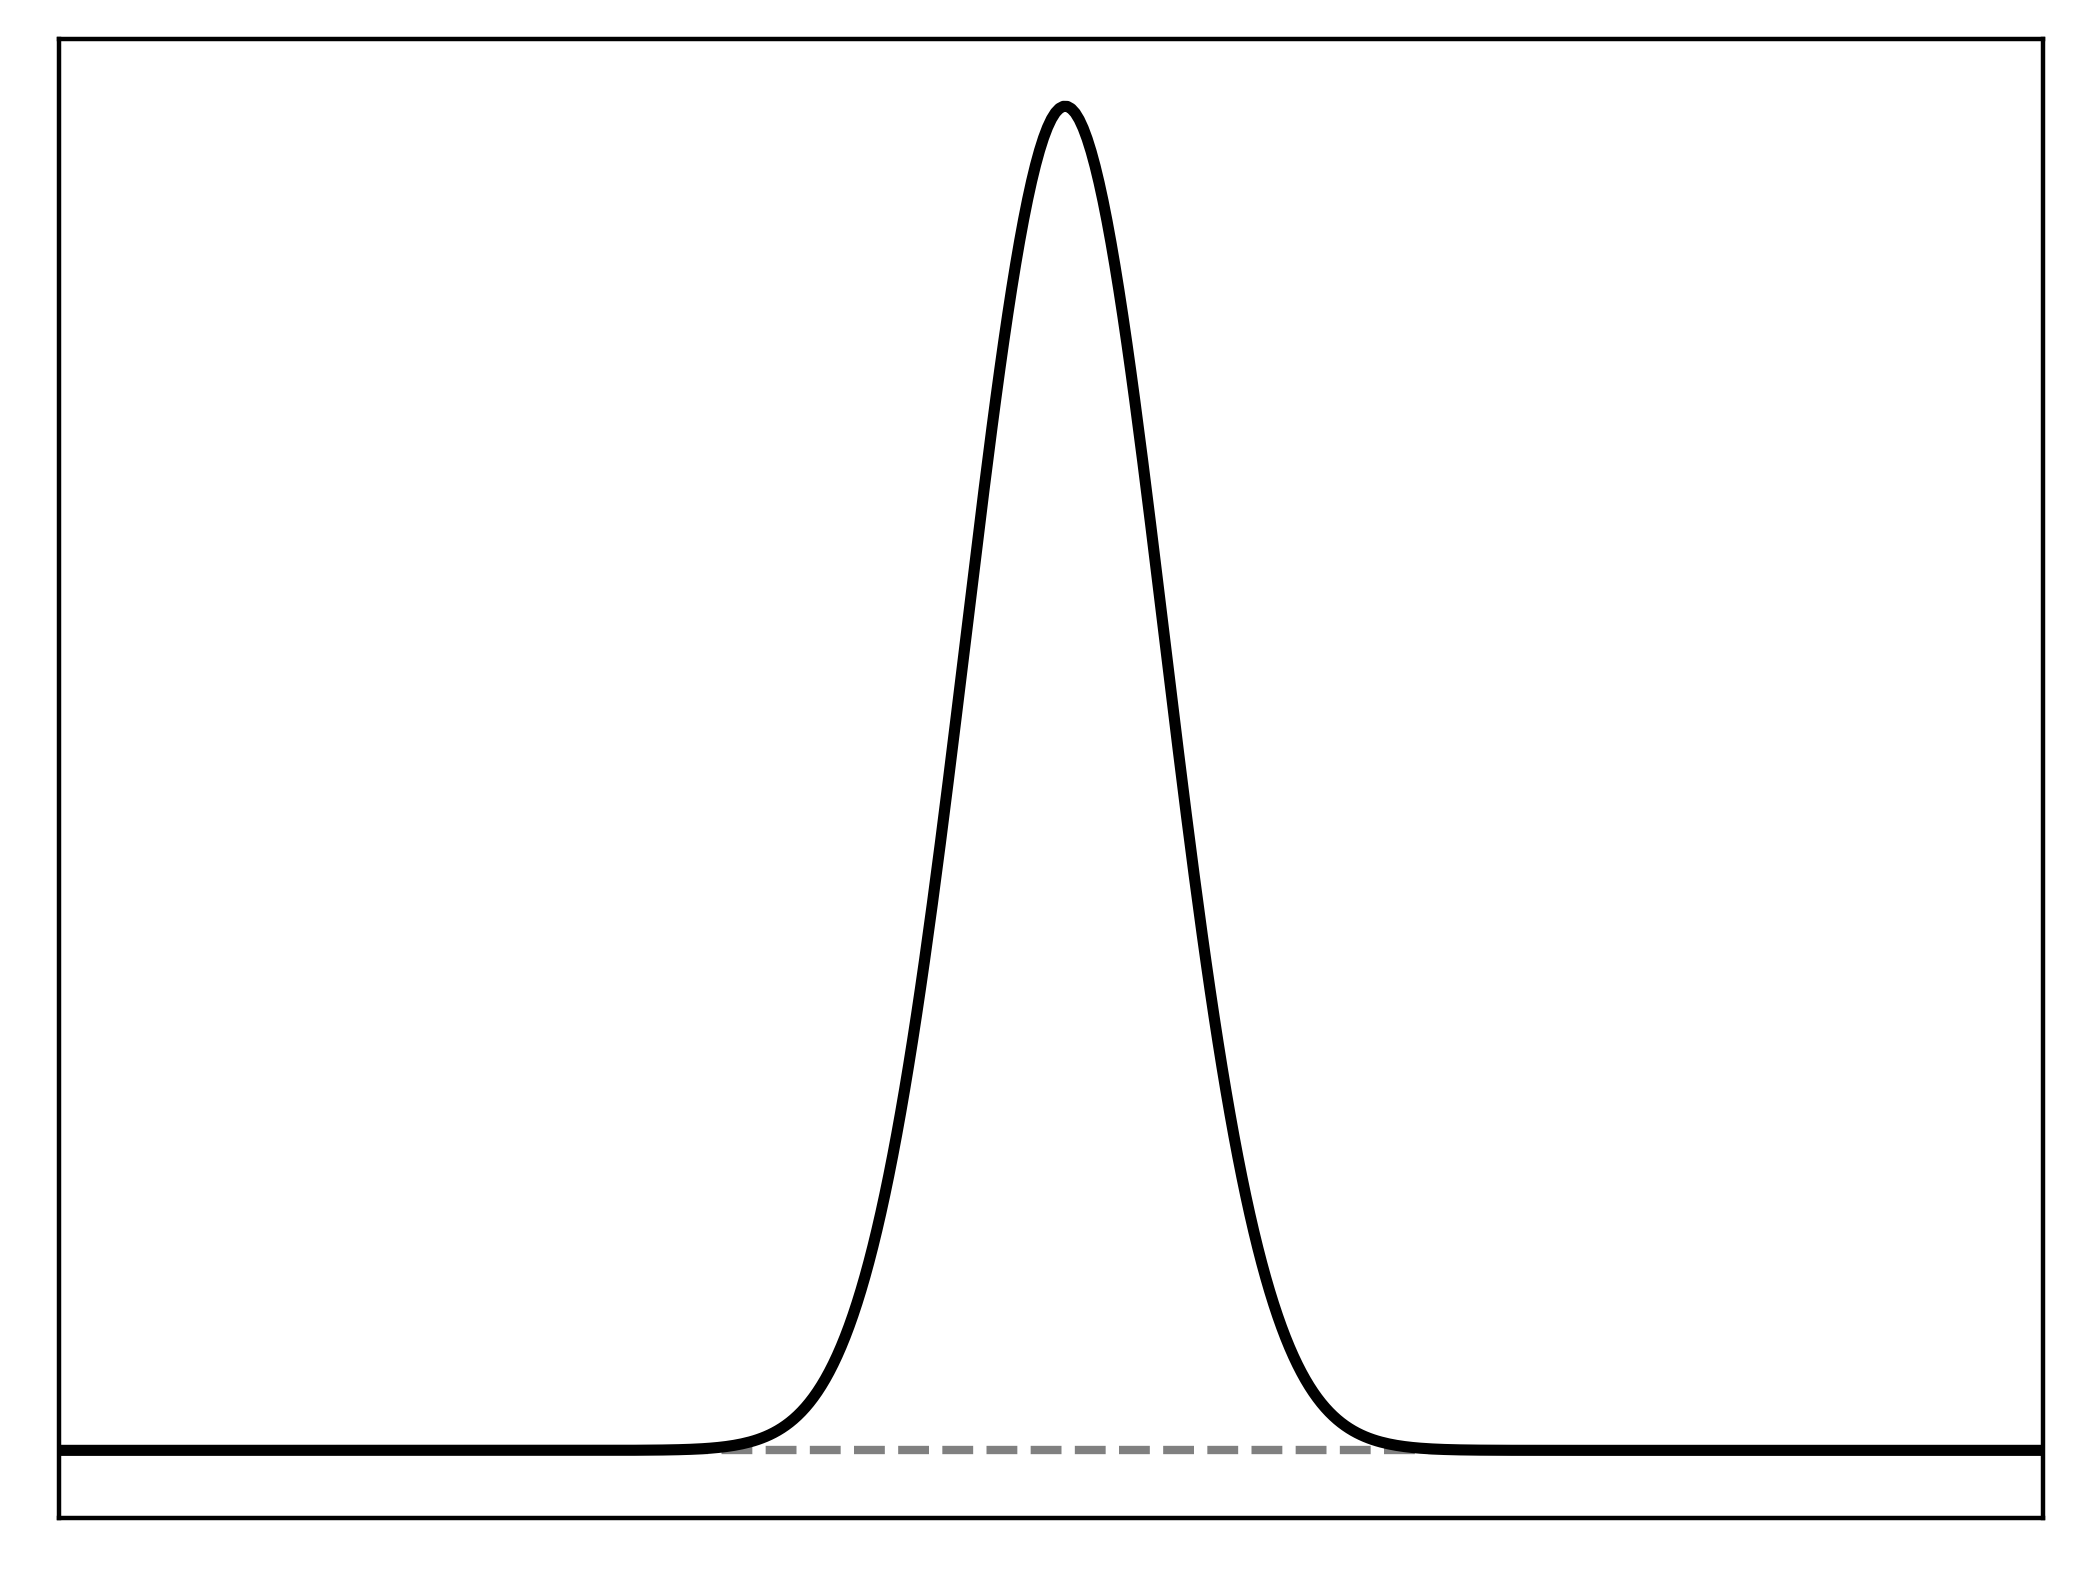
\includegraphics[scale=0.2]{localpsf_revised_figures/ricker_1d_a=0.0.png} \\
	    %
	    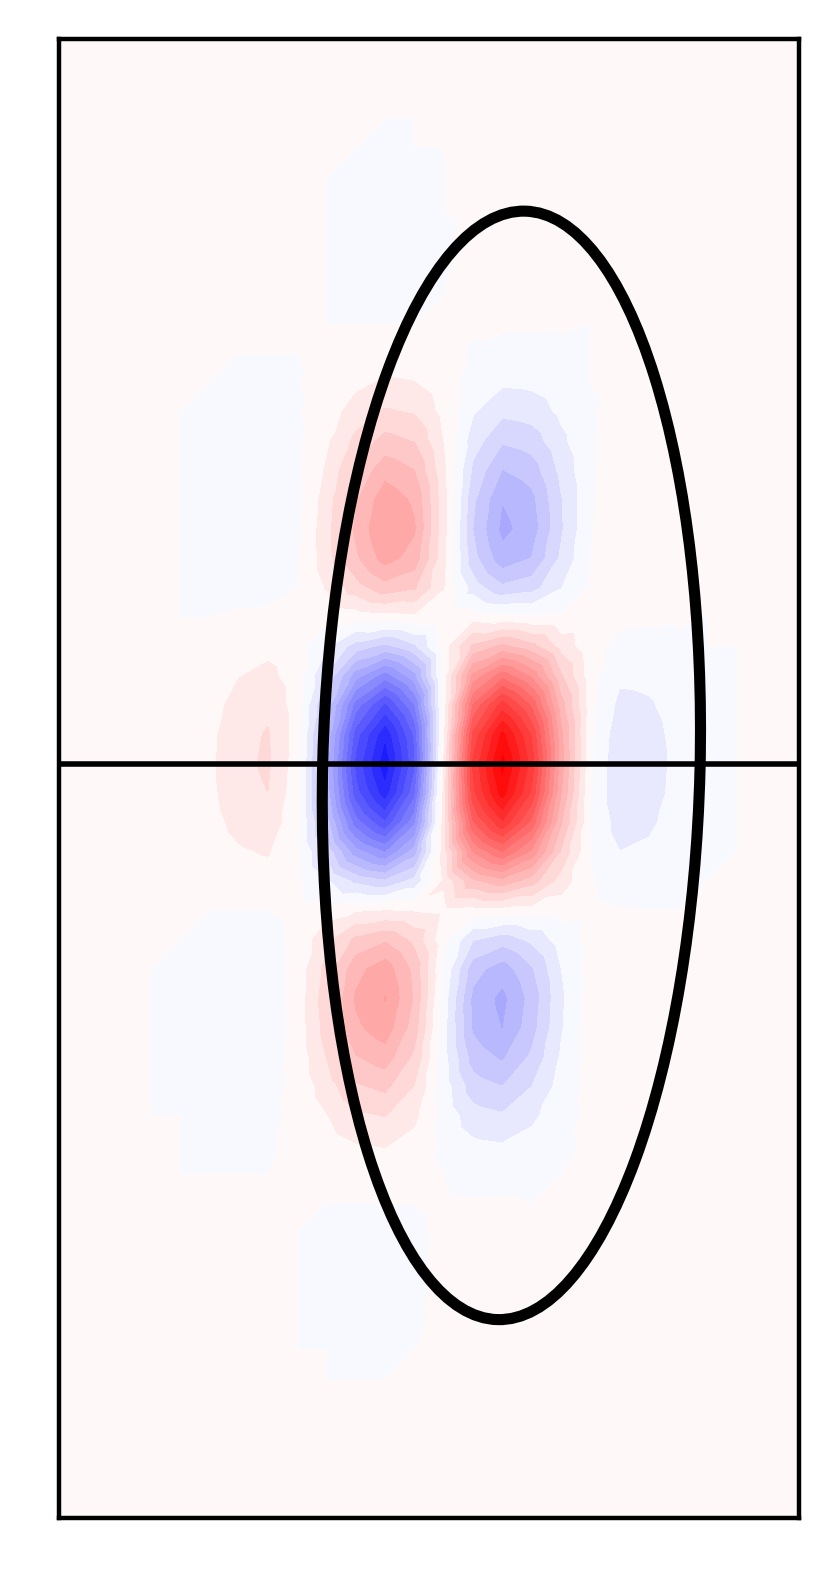
\includegraphics[scale=0.2]{localpsf_revised_figures/frog_ellipsoid_a=20.0.png} & 
	    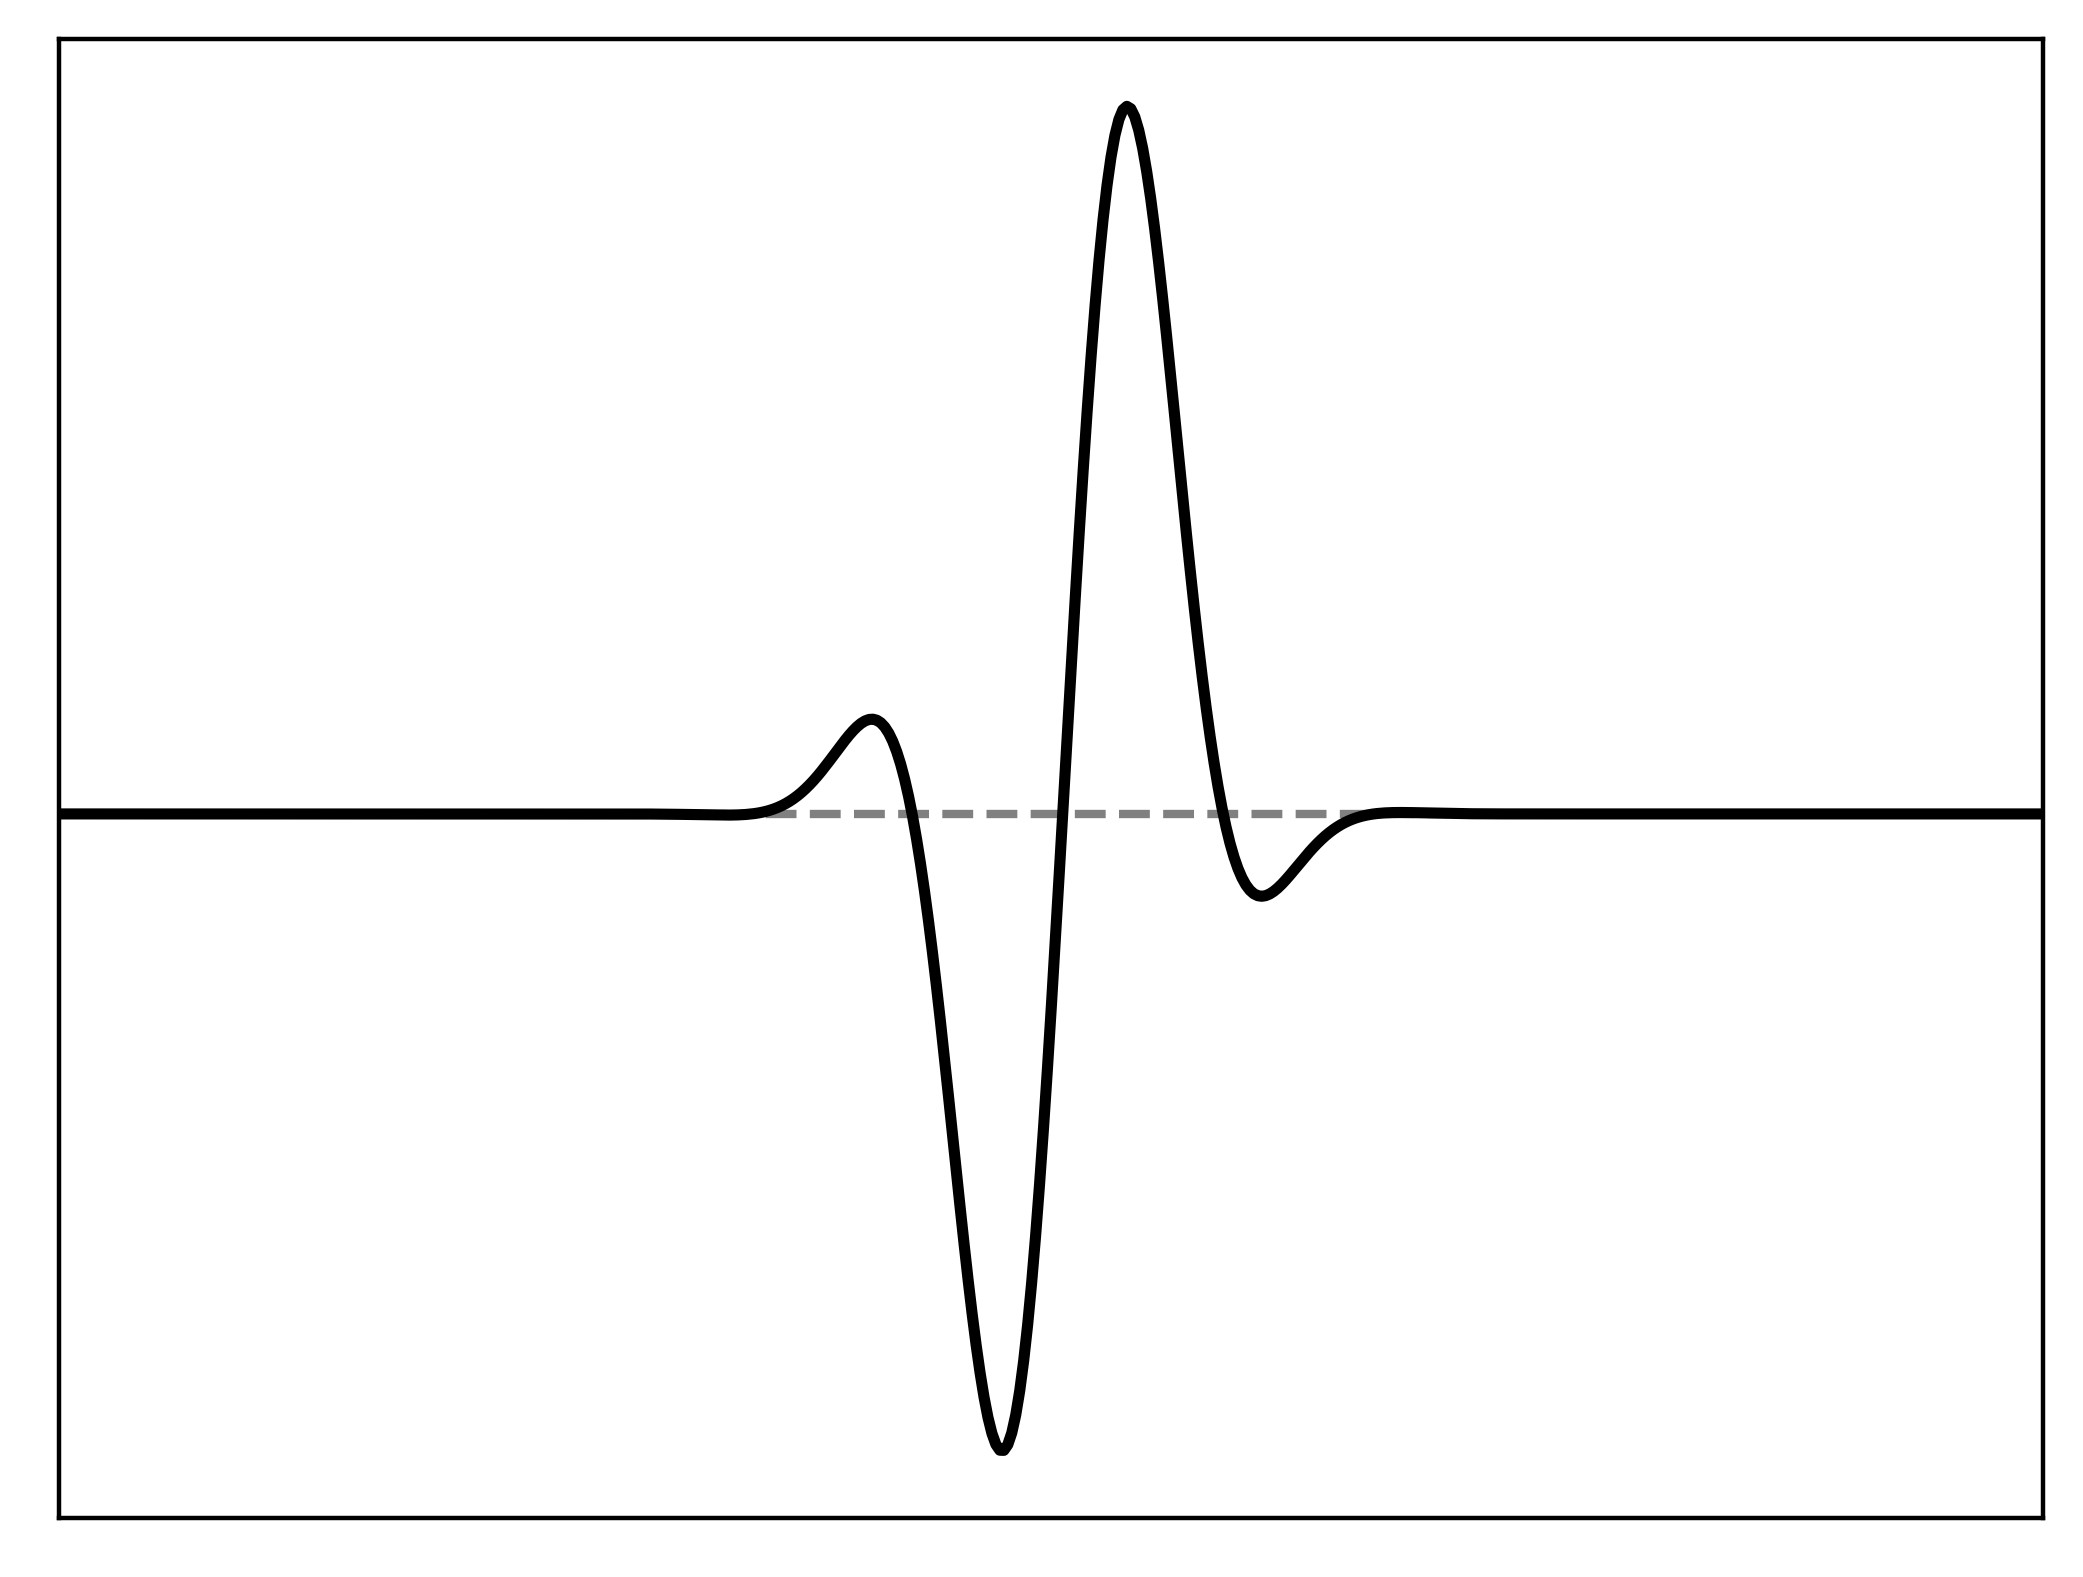
\includegraphics[scale=0.2]{localpsf_revised_figures/frog_1d_a=20.0.png} & 
	    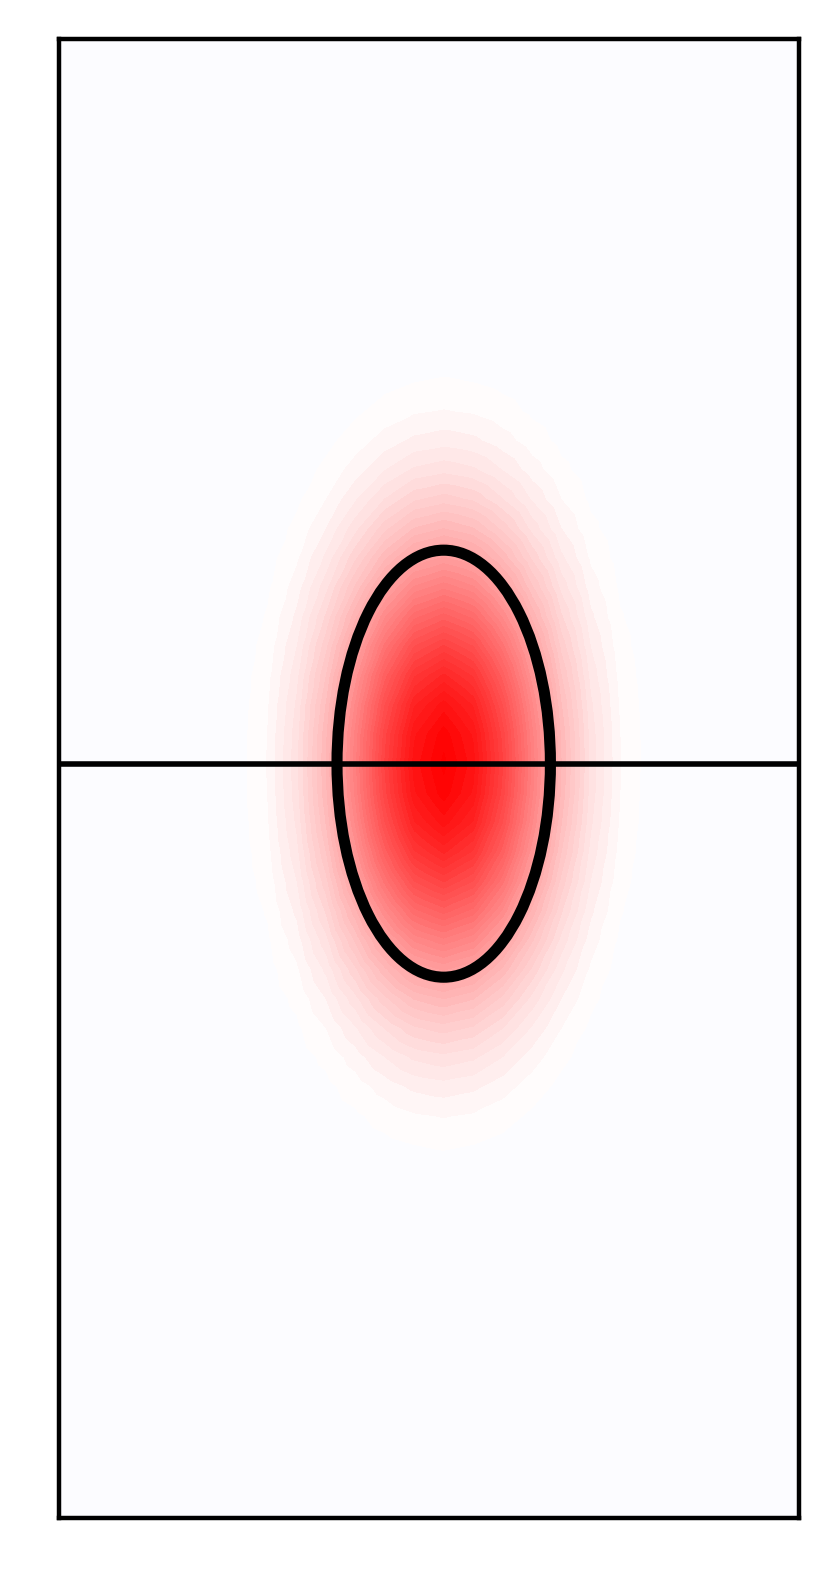
\includegraphics[scale=0.2]{localpsf_revised_figures/ricker_ellipsoid_a=0.23.png} & 
	    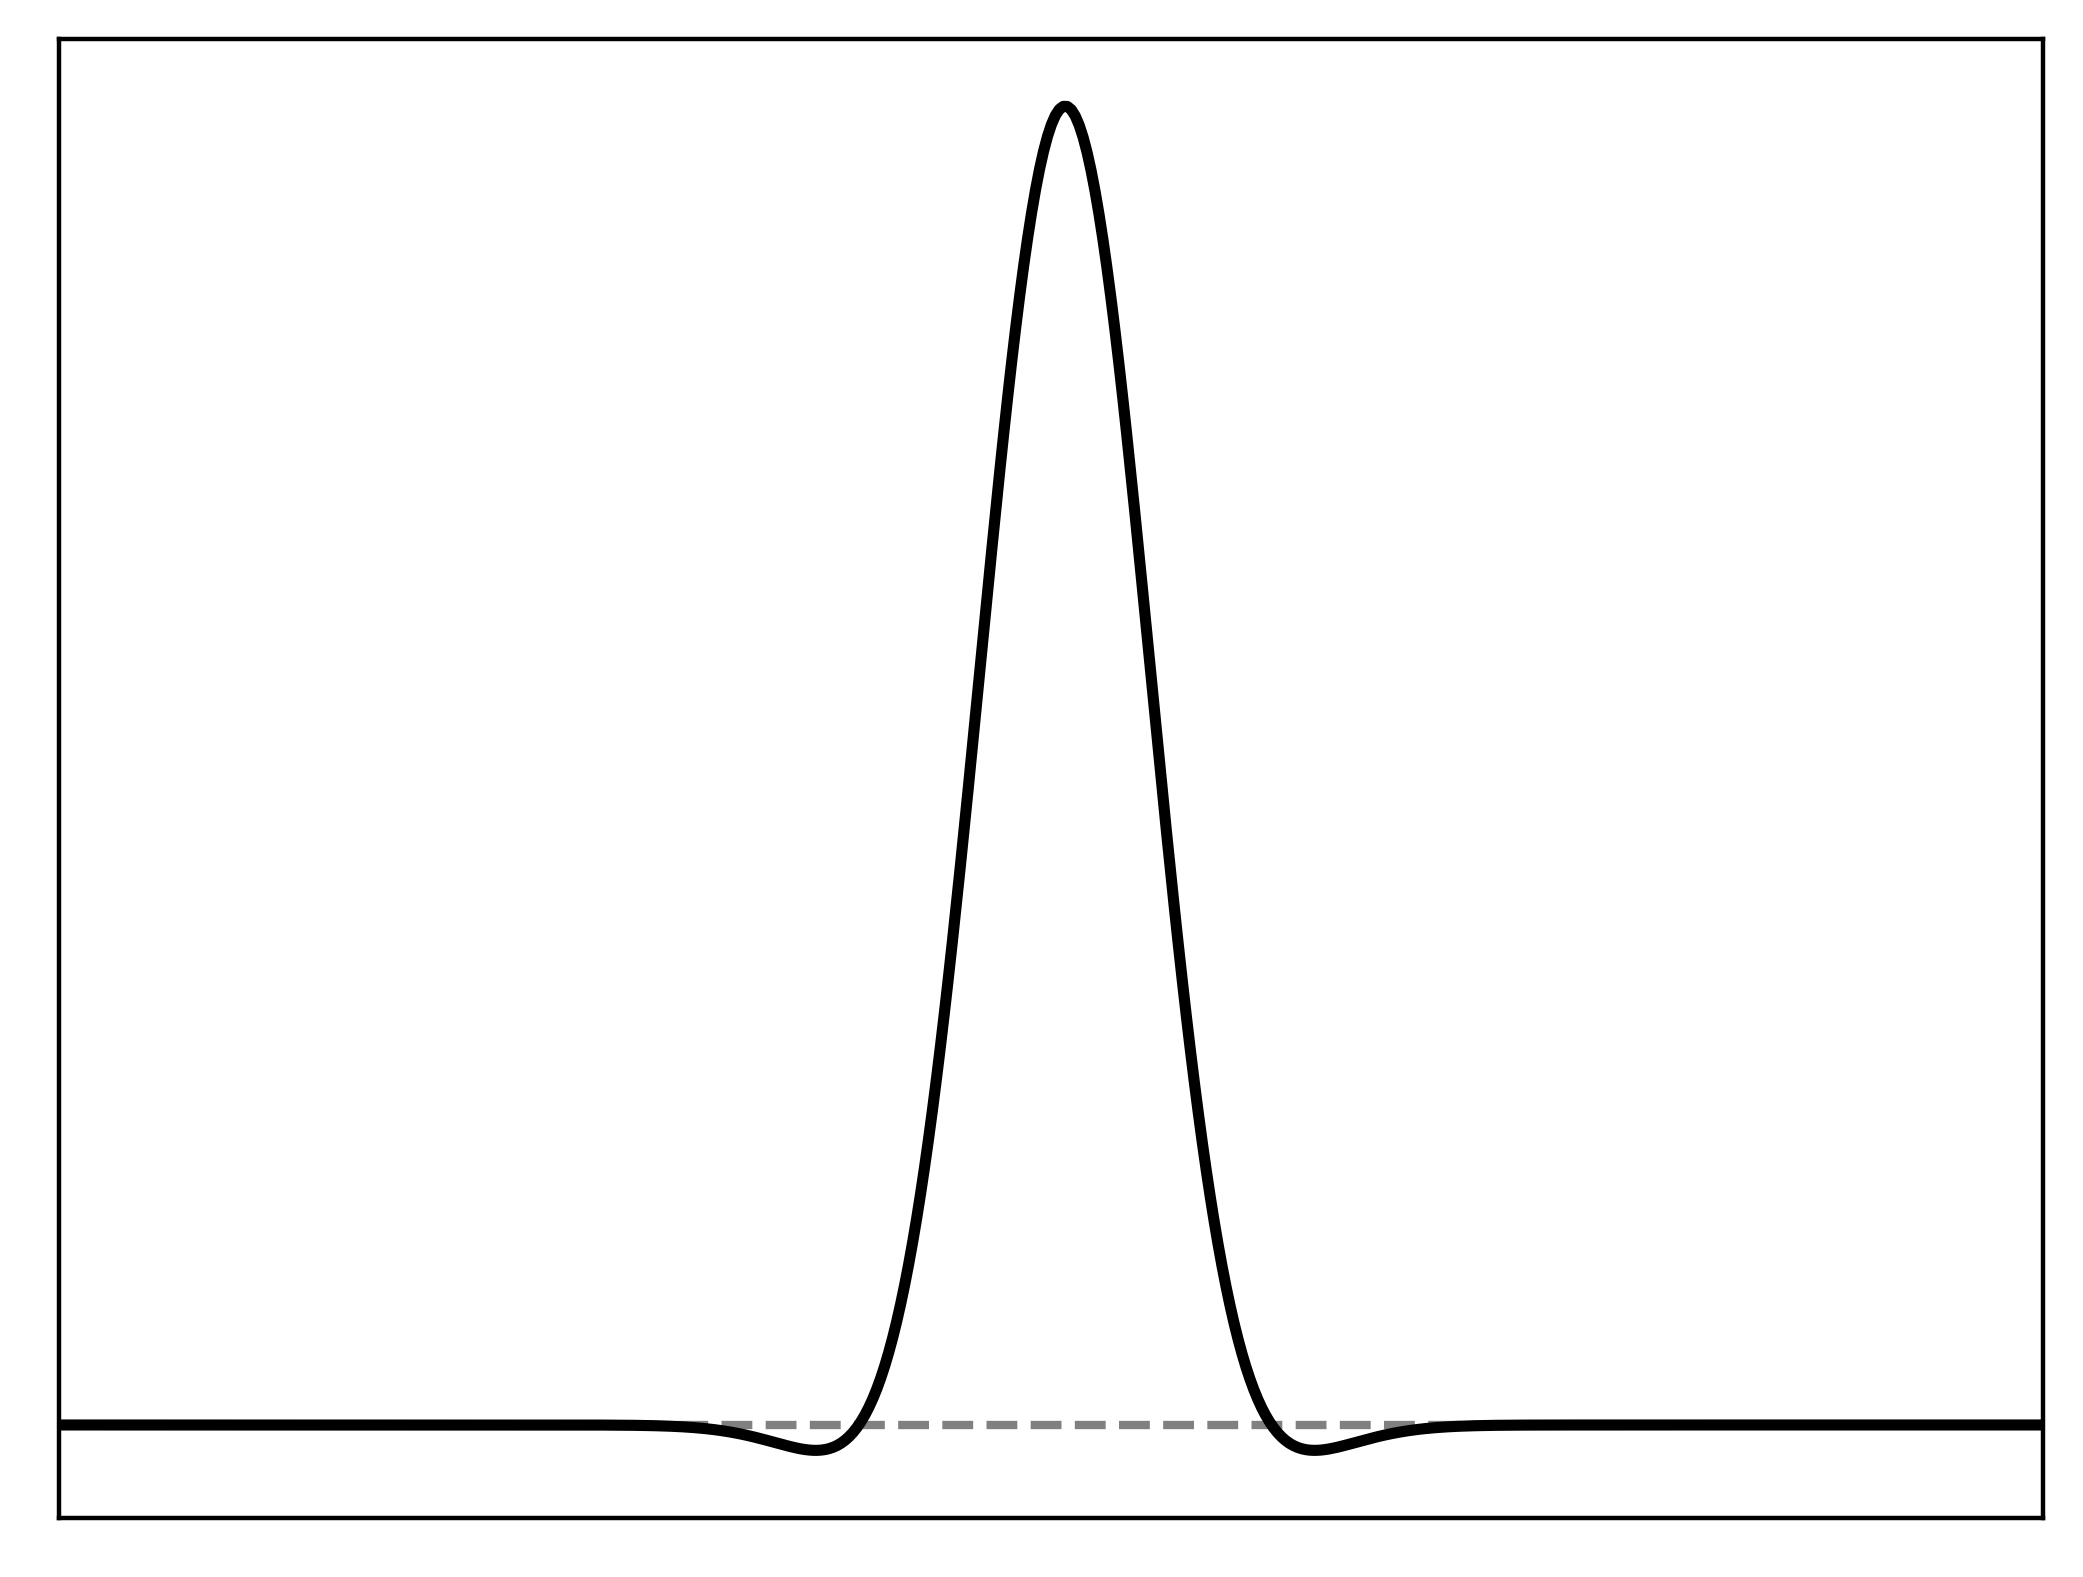
\includegraphics[scale=0.2]{localpsf_revised_figures/ricker_1d_a=0.23.png} \\
	    %
	    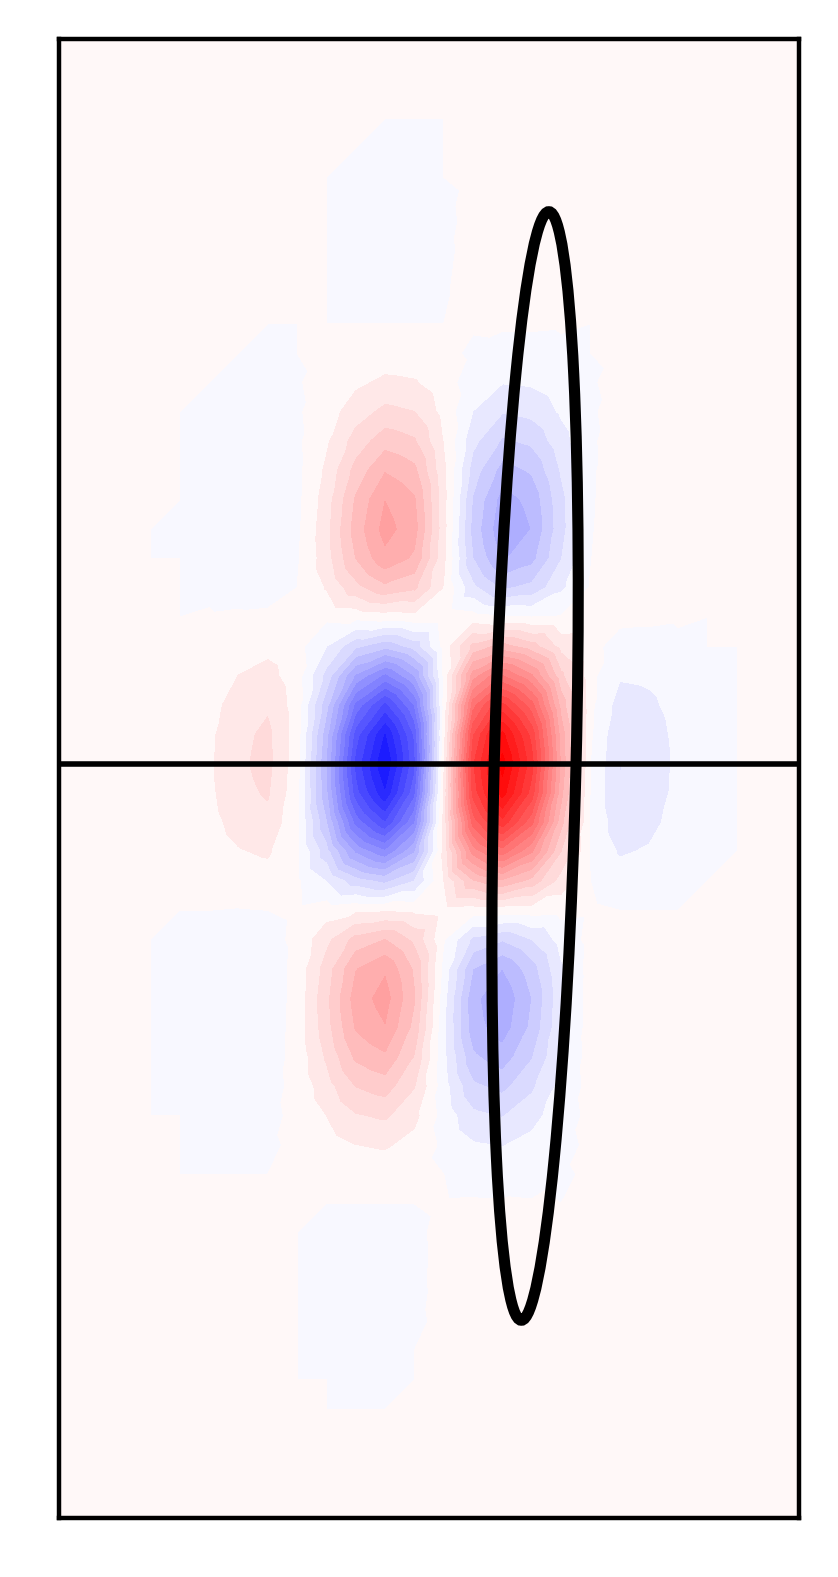
\includegraphics[scale=0.2]{localpsf_revised_figures/frog_ellipsoid_a=27.0.png} & 
	    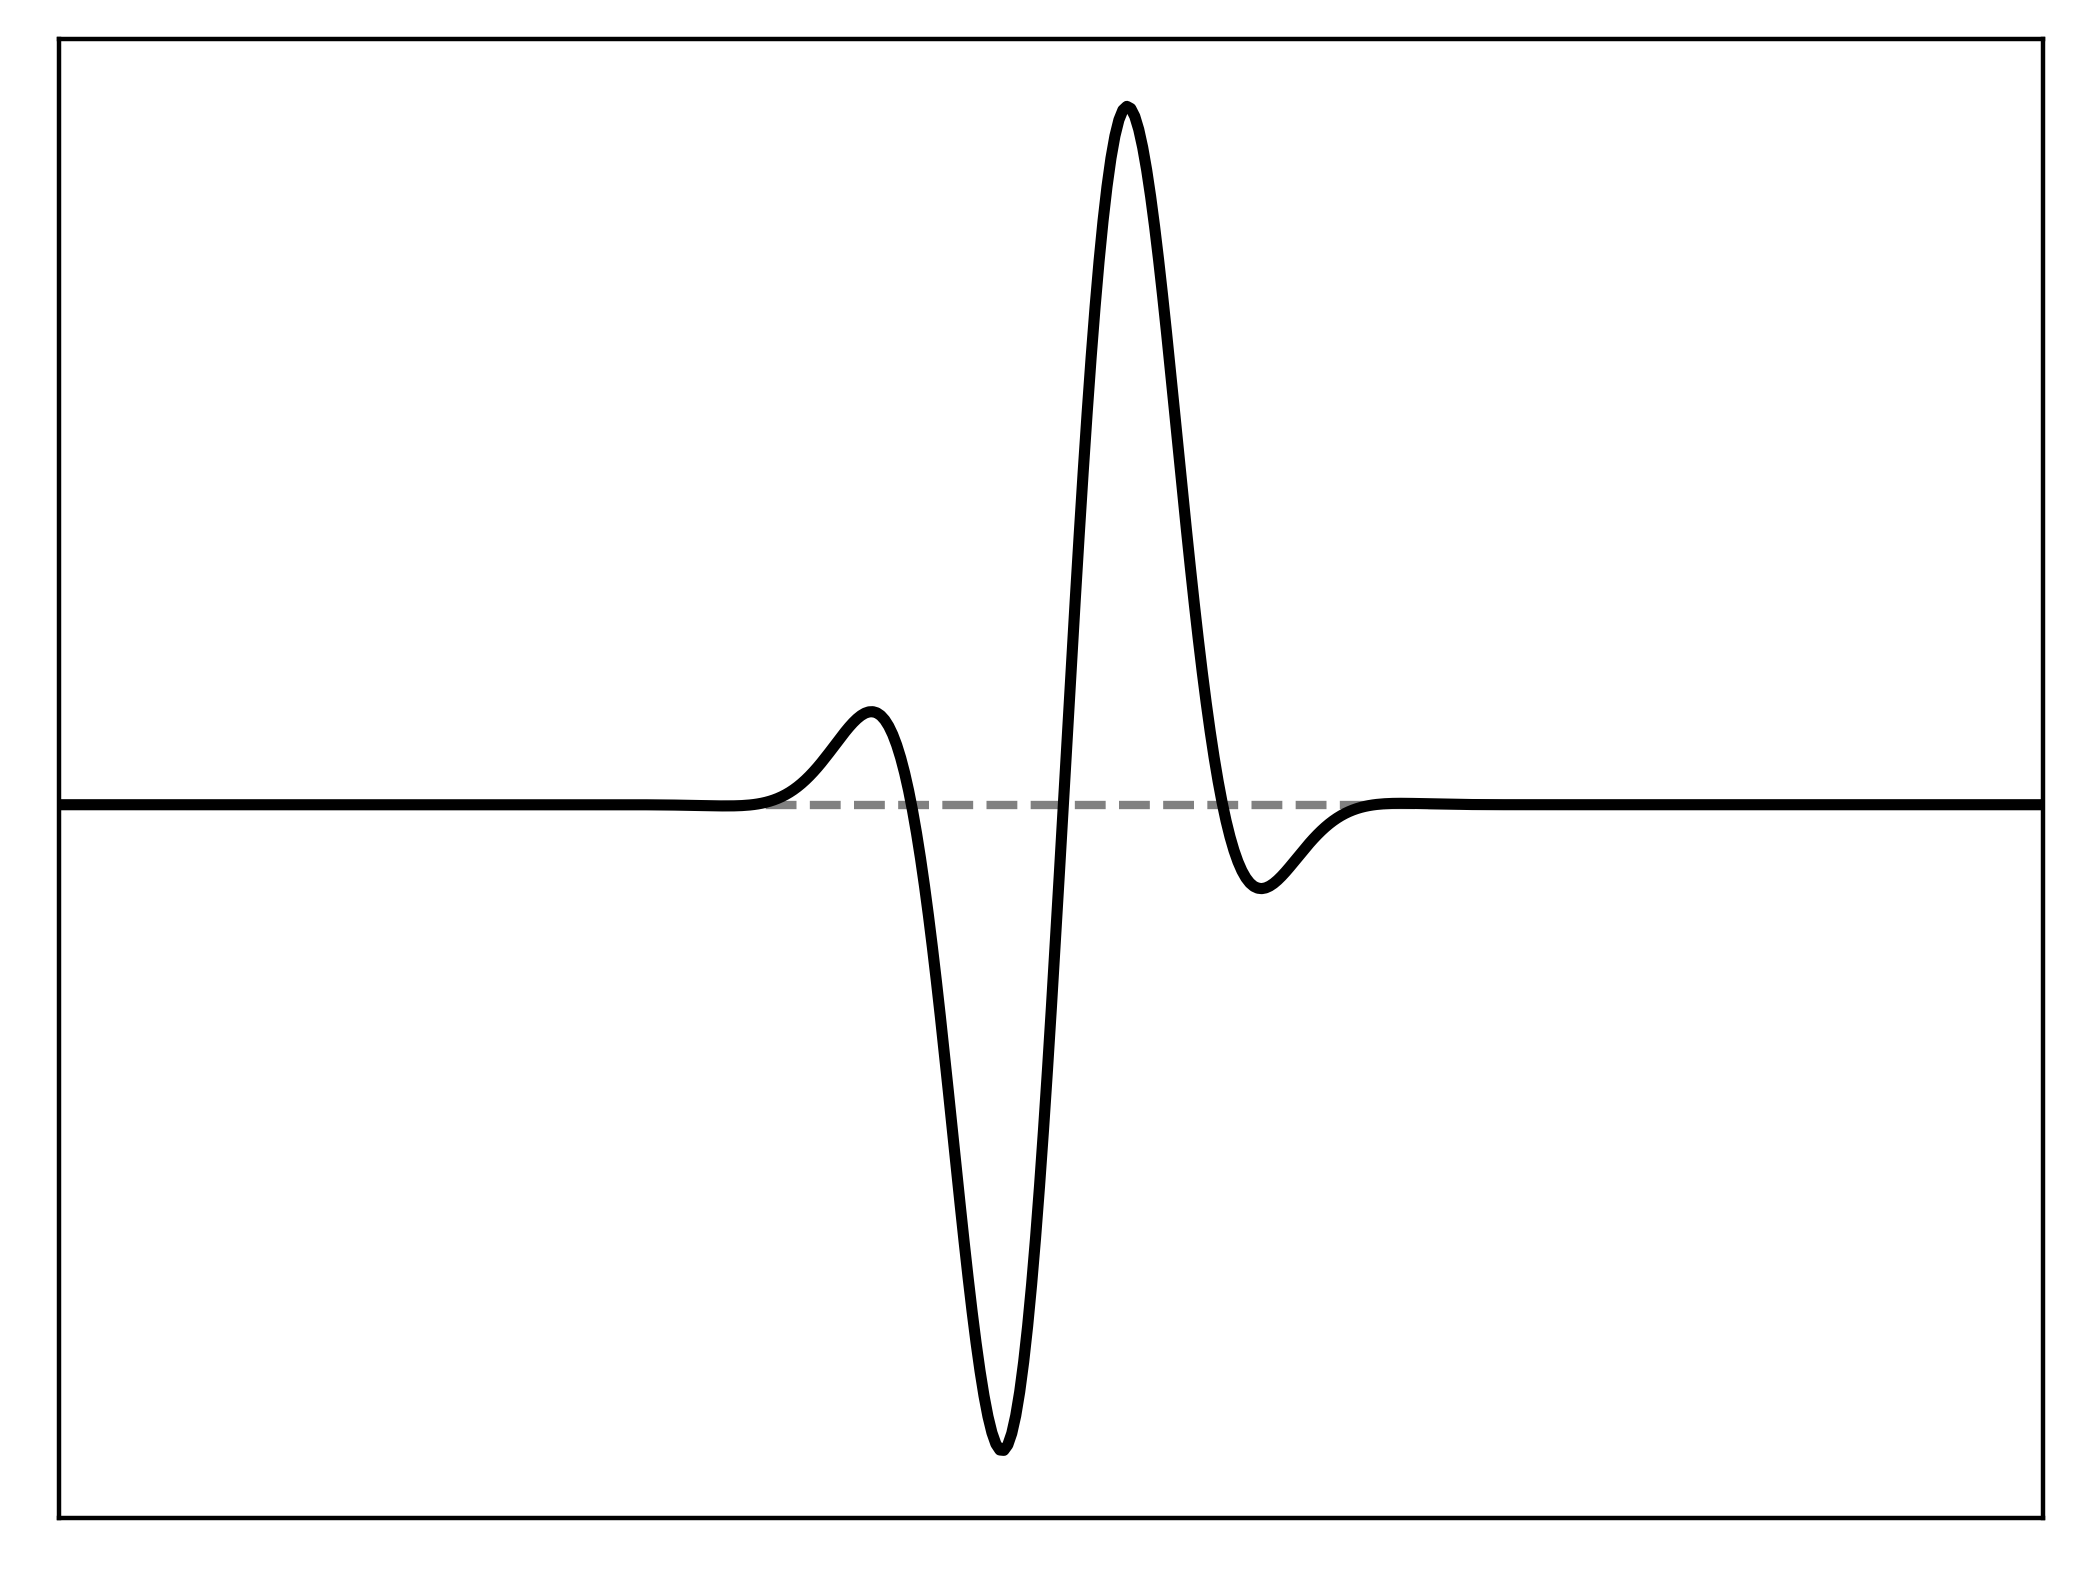
\includegraphics[scale=0.2]{localpsf_revised_figures/frog_1d_a=27.0.png} & 
	    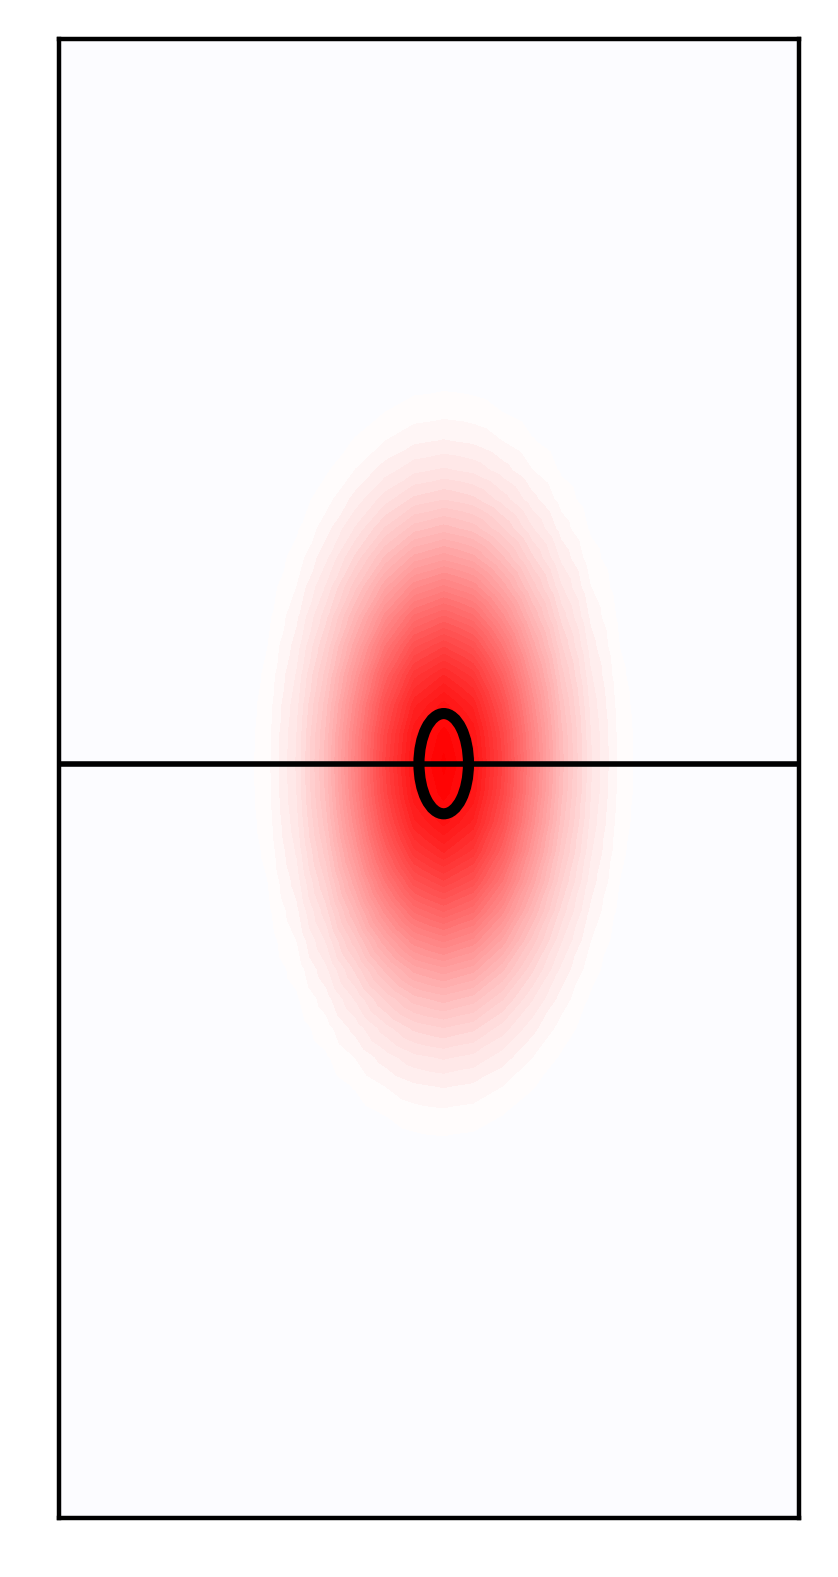
\includegraphics[scale=0.2]{localpsf_revised_figures/ricker_ellipsoid_a=0.249.png} & 
	    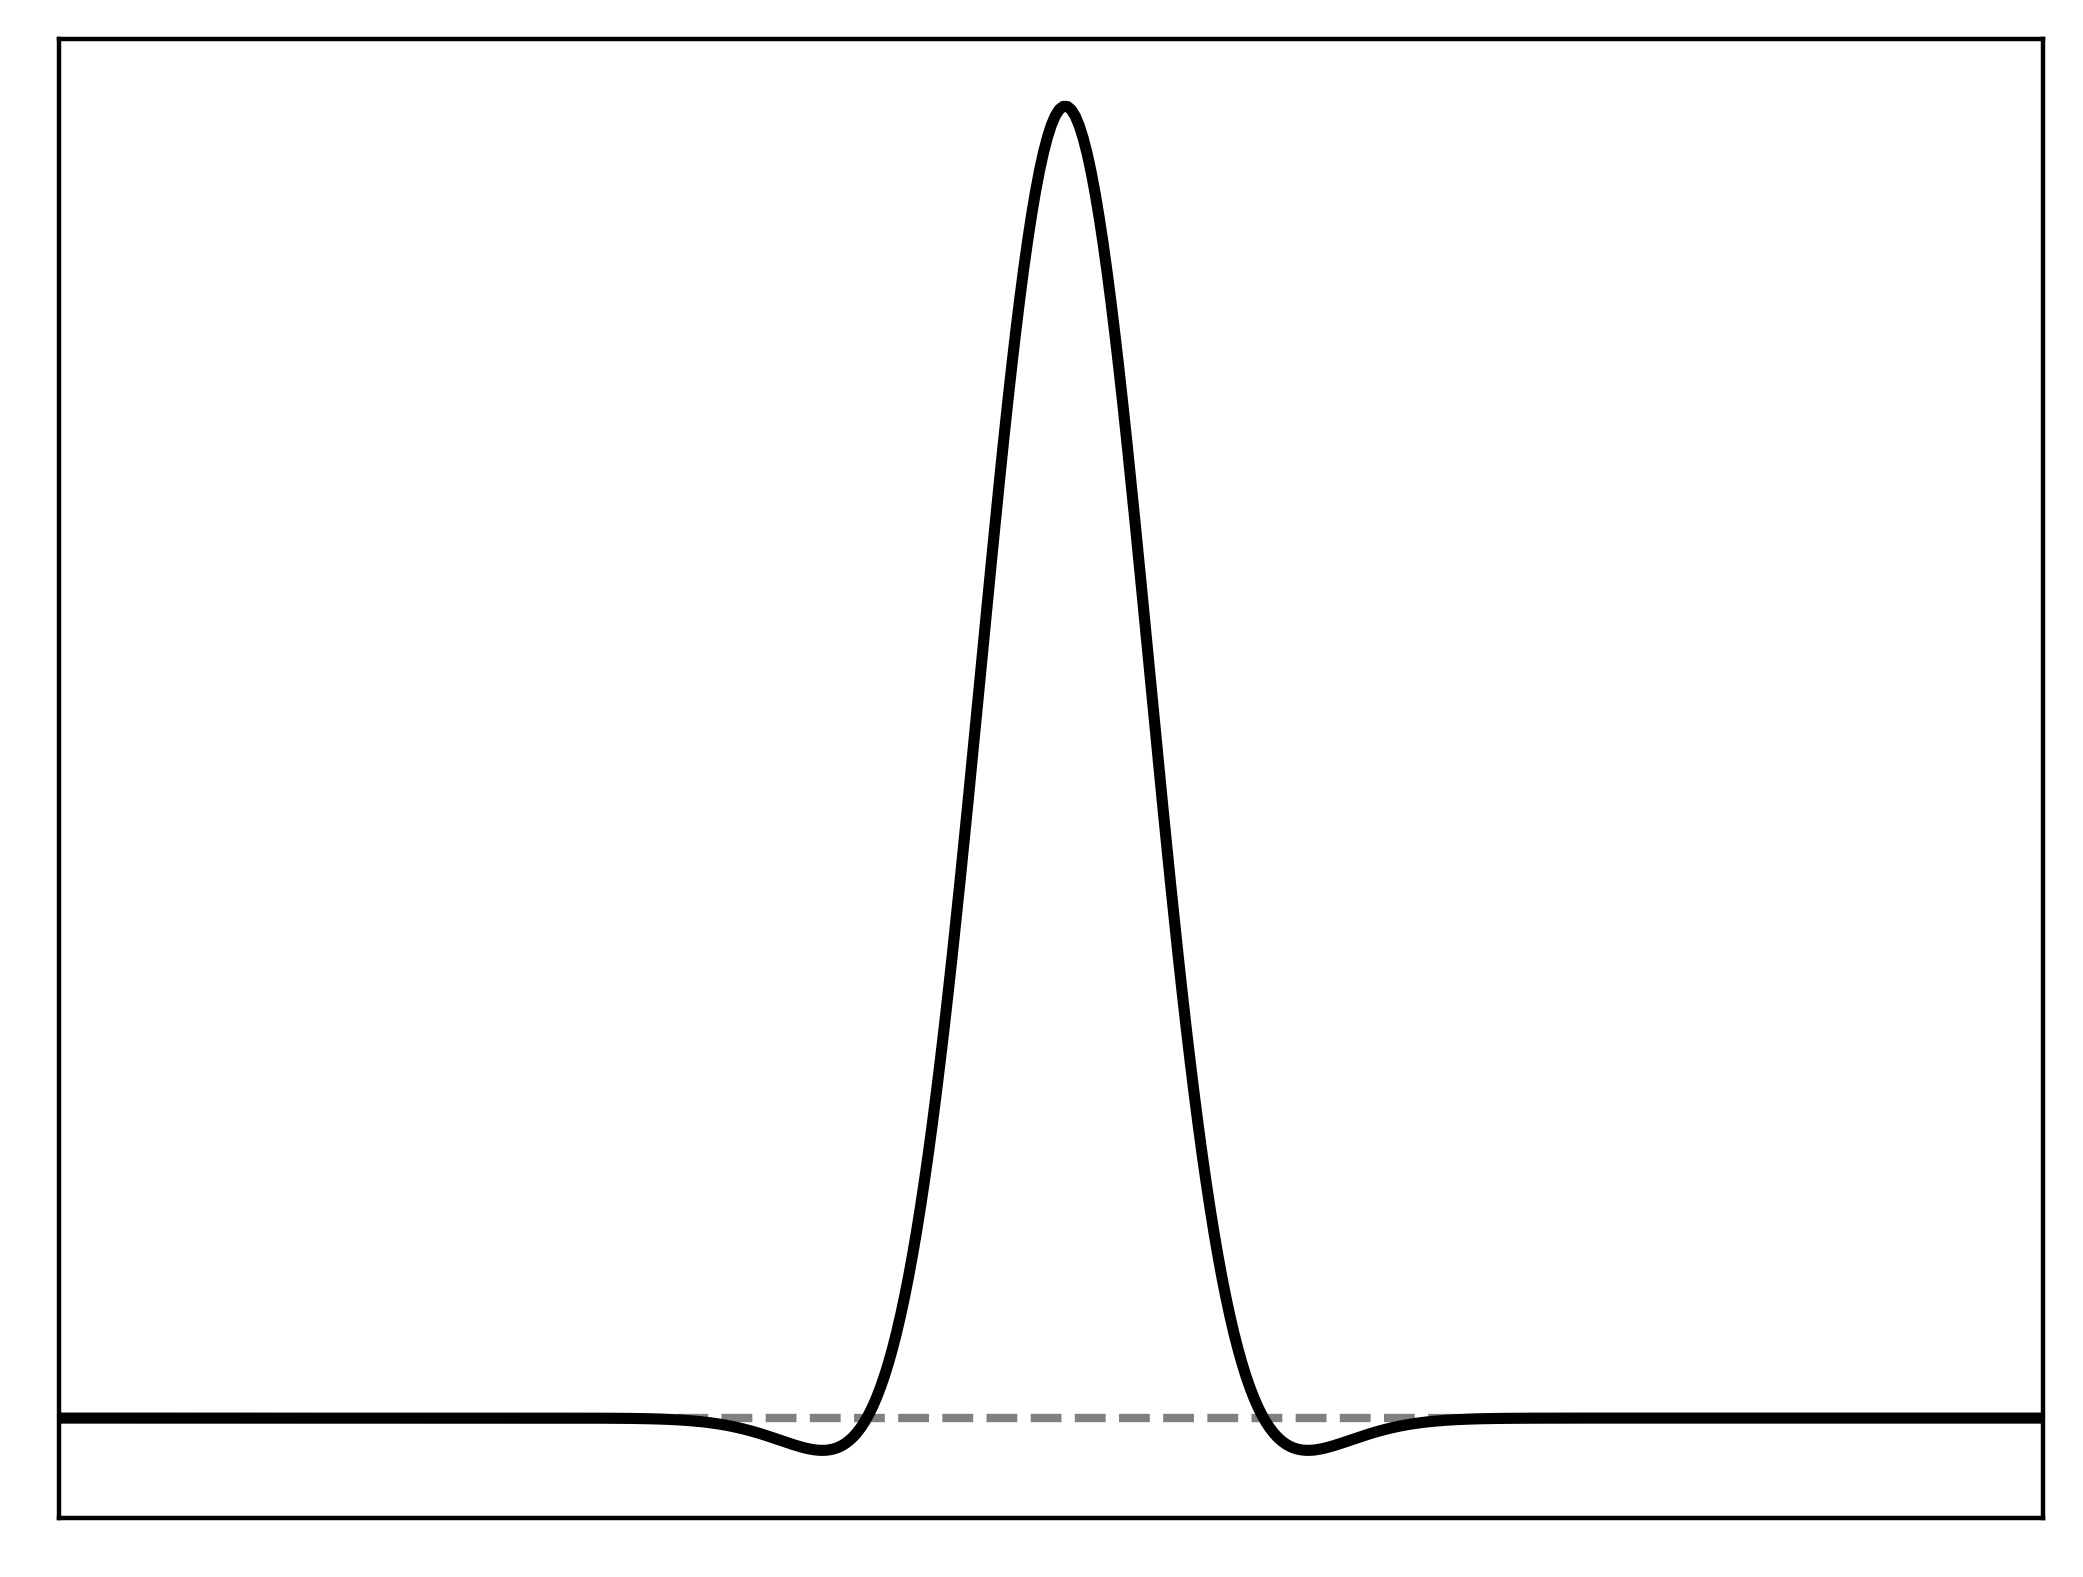
\includegraphics[scale=0.2]{localpsf_revised_figures/ricker_1d_a=0.249.png} 
	  \end{tabular}
	}
	%\caption{Illustration of the influence of negative numbers in
        %  the integral kernel on the robustness of the ellipsoid
        %  estimates for the supports of impulse responses. Left two
        %  columns: spatially variant blur kernel given in Equation
        %  \ref{eq:frog_kernel}. Right two columns: Ricker wavelet-type
        %  kernel given by $\Aker(y,x) = (1 - a
        %  \gamma)\exp\left(-\gamma/2\right)$, where $\gamma=(y-x)^T
        %  \Sigma^{-1} (y-x)$, and
        %  $\Sigma=\operatorname{diag}\left(0.0025,
        %  0.01\right)$. Ordered from top to bottom, the results are
        %  obtained with $a\in\{1.0, 20.0, 27.0\}$ for the left two
        %  columns, and $a\in \{0.0, 0.23, 0.249\}$ for the right two
        %  columns. Columns 1 and 3: impulse responses with estimated
        %  support ellipsoids indicated by the black ellipses. Red and
        %  blue represent positive and negative numbers in the integral
        %  kernel, respectively. Columns 2 and 4: one-dimensional slice
        %  along the horizontal line indicated in the two-dimensional
        %  plots. The dashed gray line is at zero.  }
	%\label{fig:robustness_to_negatives}
  \end{figure}
  
  \begin{center}
    Spatially variant blur kernel (left two columns) and a Ricker
    wavelet-type kernel (right two columns) for progressively more
    significant negative numbers in the integral kernel (top to
    bottom).
  \end{center}

\end{frame}

%---------------------------------------------------------------------
\begin{frame}
  \frametitle{Relative error in the PSF approximation of the kernel}
  %\framesubtitle{Relative error in the PSF approximation of the kernel}

  \begin{figure}
	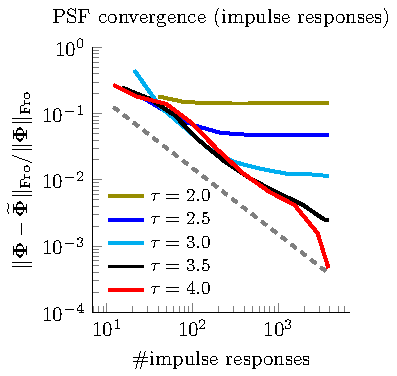
\includegraphics[scale=0.96]{localpsf_revised_figures/frog_tau_impulses.pdf}
	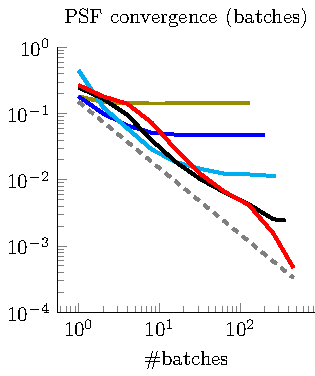
\includegraphics[scale=0.96]{localpsf_revised_figures/frog_tau_batches.pdf}
  \end{figure}

  \begin{center}
    Left: Relative error vs. the total number of impulse responses
    used in the approximation. Right: Relative error vs. the number of
    impulse response batches.The dashed gray lines show linear
    convergence rates.
  \end{center}
 
\end{frame}
%---------------------------------------------------------------------
%\begin{frame}
%  \frametitle{Exploiting the problem structure}
%  \framesubtitle{Local mean-displacement invariance}
%  
%  \begin{figure}
%	\centering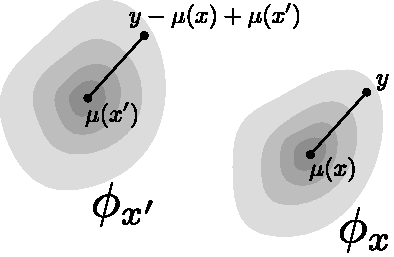
\includegraphics[scale=0.75]{figures/mean_displacement_invariance.pdf}
%  \end{figure}
%
%  \begin{center}
%    Impulse responses that arise from applying $\Aop$ to point sources \\at two points, $x$ and $x'$.
%  \end{center}
%   %\footnotesize
%   \begin{itemize}
%   \item The operator $\Aop$ is locally mean displacement invariant if
%     $\impulseresponse_{x}(y) \approx \impulseresponse_{x'}\left(y -
%     \spatialmean(x) + \spatialmean(x')\right)$ when $x$ is close to
%     $x'$.
%   \item Here $\spatialmean(z)$ denotes the mean (center of mass) of $\phi_z$.
%   \end{itemize}
%
%\end{frame}
%---------------------------------------------------------------------
\begin{frame}
  \frametitle{Example: Ice sheet inverse problem}

  \begin{figure}
	\centering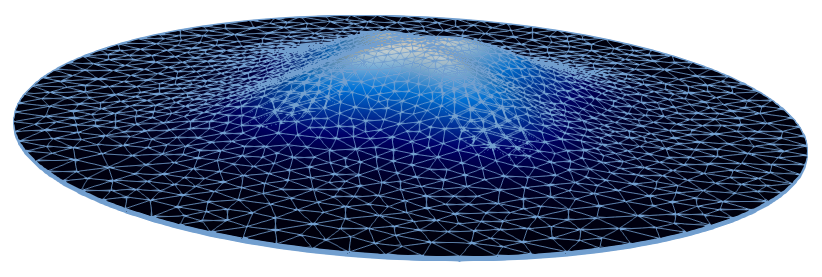
\includegraphics[scale=0.22]{figures/meshHeight_view2_edges.png}\\
	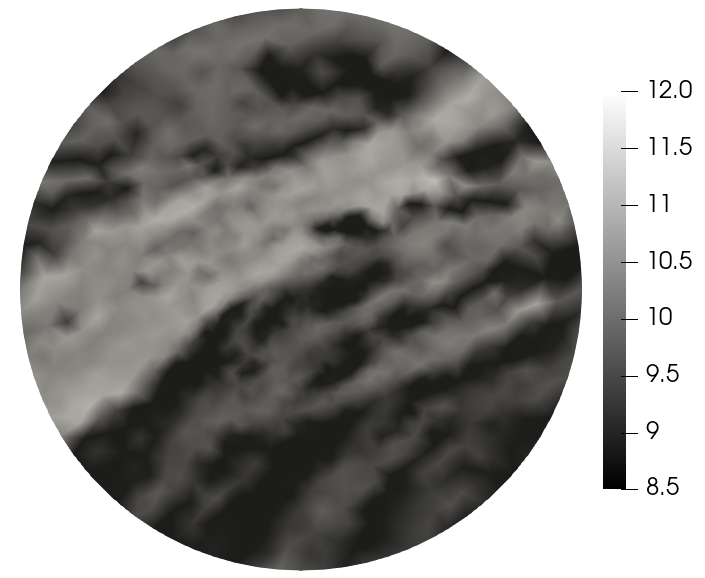
\includegraphics[scale=0.18]{figures/mtrue_withColorBar.png}
	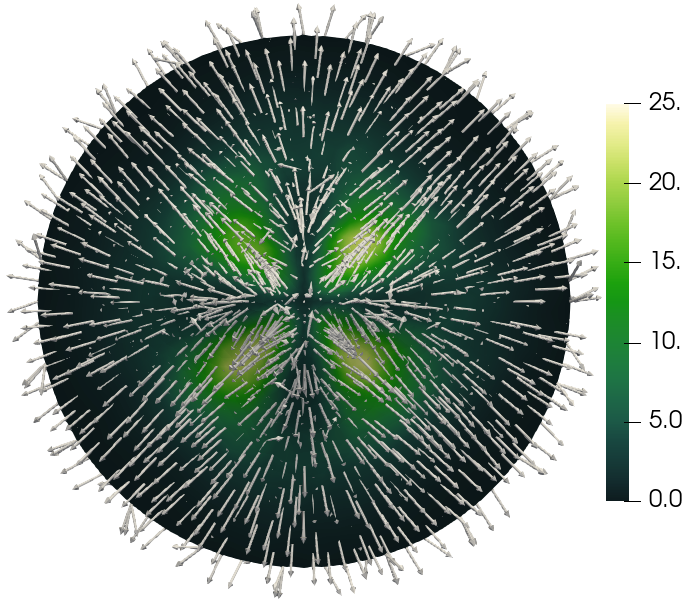
\includegraphics[scale=0.18]{figures/trueVelocity2_glyphs.png}
  \end{figure}
  \begin{center}
    The ice sheet geometry and discretization (top), the ``true''
    parameter (bottom left) and the corresponding velocity field
    (bottom right).
  \end{center}
\end{frame}
%---------------------------------------------------------------------
\begin{frame}
  \frametitle{Example: Ice sheet inverse problem}
  \framesubtitle{Impulse responses}

  \begin{figure}
	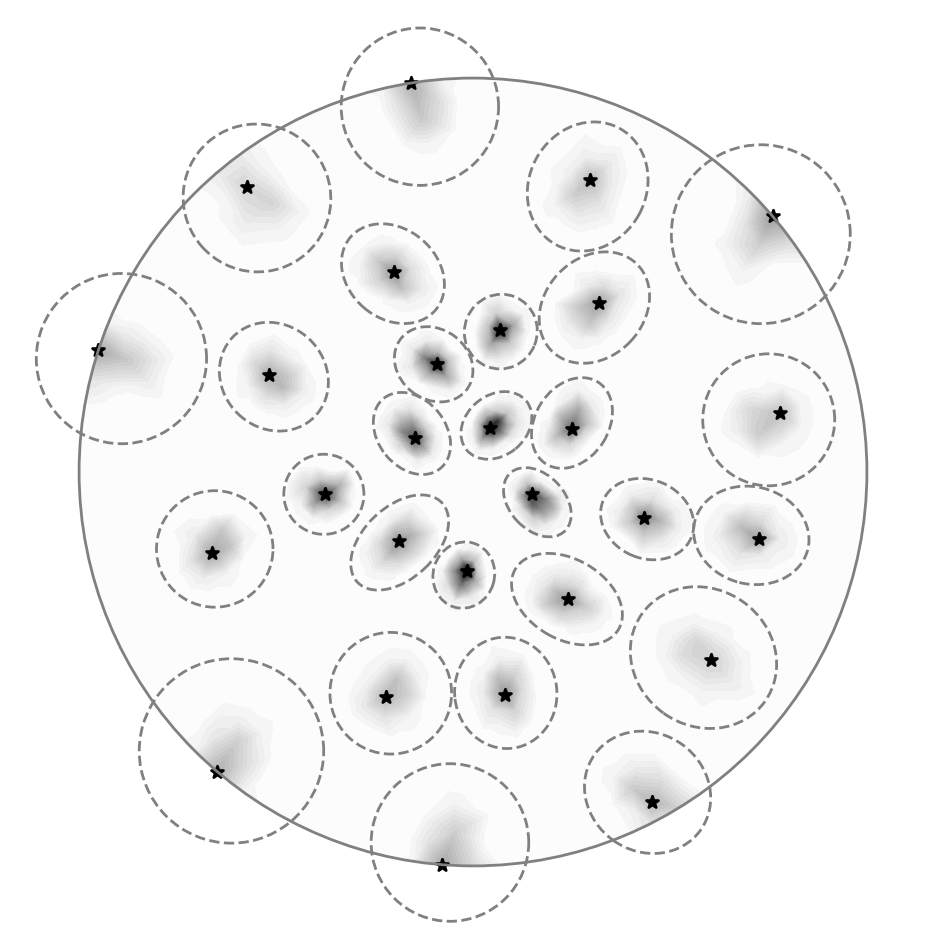
\includegraphics[width=0.32\columnwidth]{figures/impulse_batch1.png}
	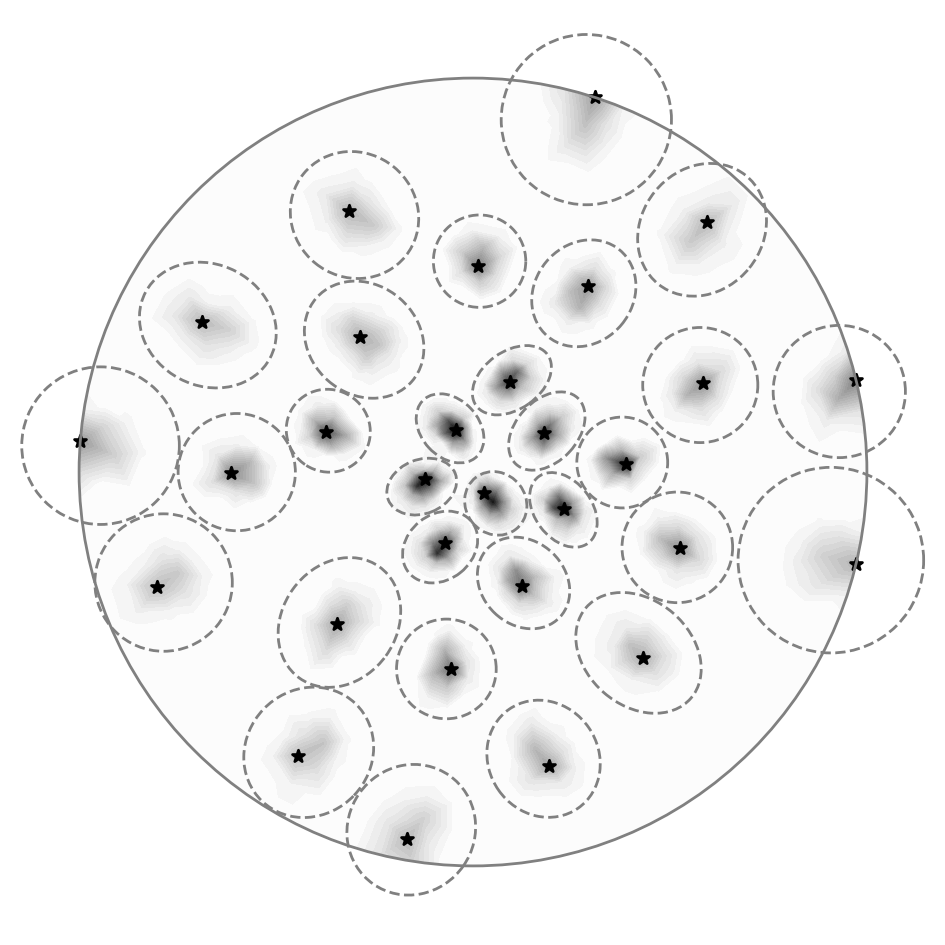
\includegraphics[width=0.32\columnwidth]{figures/impulse_batch2.png}
	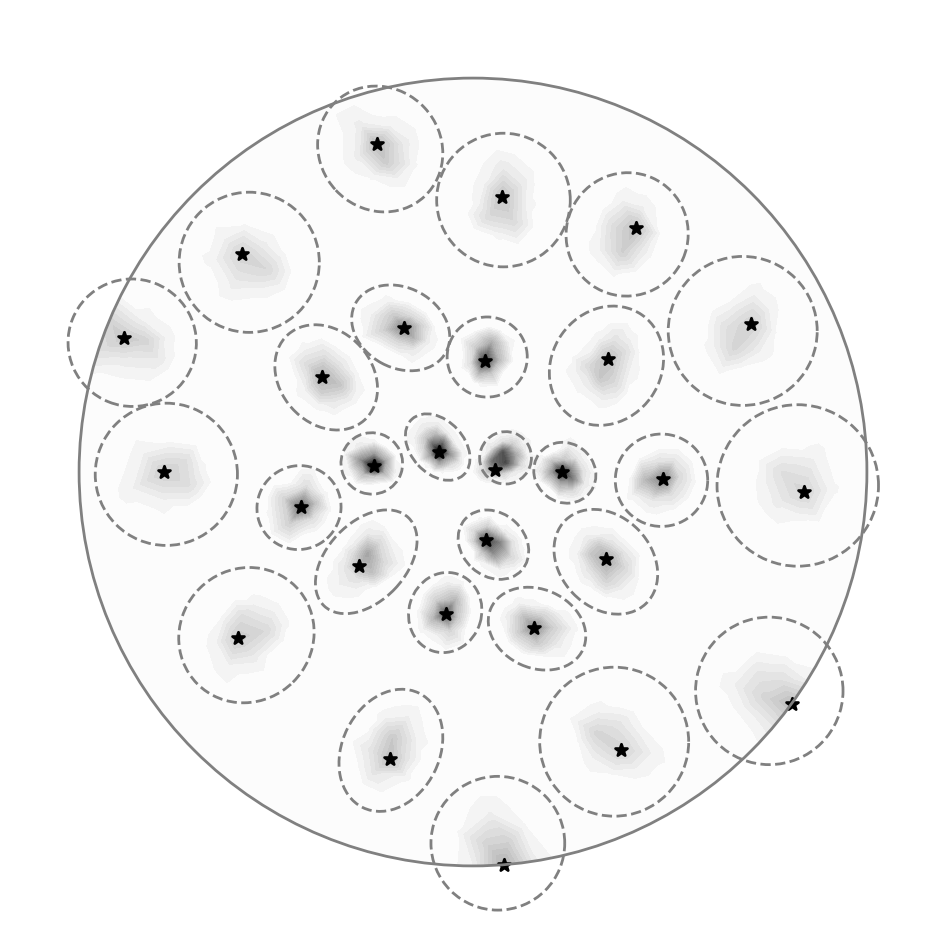
\includegraphics[width=0.32\columnwidth]{figures/impulse_batch3.png}
  \end{figure}

   %\footnotesize
   \begin{itemize}
   \item Black stars are point source locations.
   \item Shading shows the magnitude of the normalized impulse
     responses (darker means larger function values).
   \item Dashed gray ellipses are estimated impulse
     response support ellipsoids based on the moment method.
   \end{itemize}

\end{frame}
%---------------------------------------------------------------------
\begin{frame}
  \frametitle{Example: Ice sheet inverse problem}

  \begin{figure}
    %[width=0.8\columnwidth]
    \centering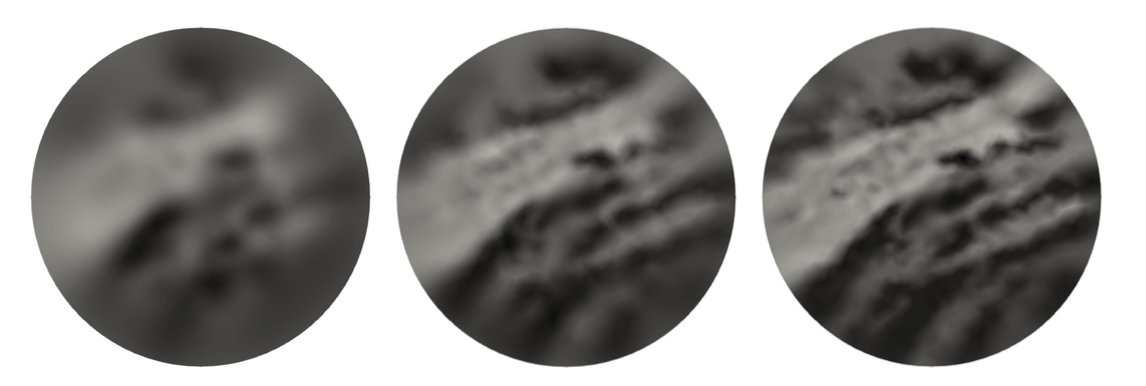
\includegraphics[scale=0.6]{extraplots/reconstructions-ice.png}
	%\centering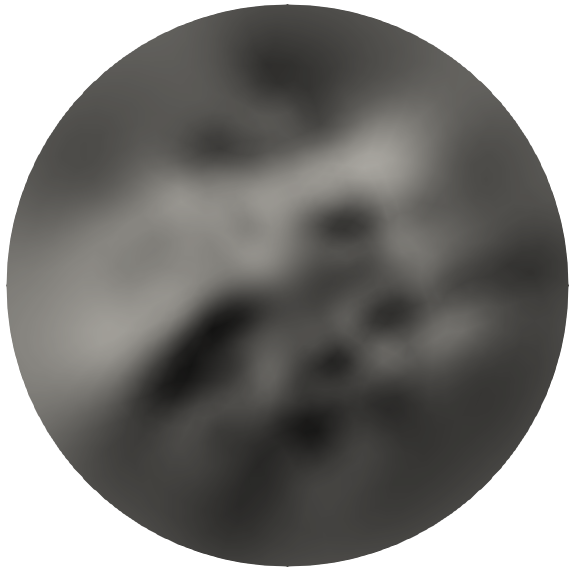
\includegraphics[scale=0.18]{figures/mstar_0.25noise_cropped.png}
	%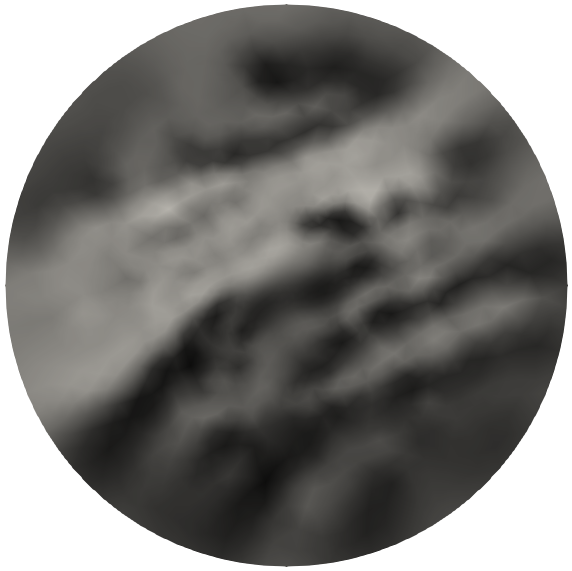
\includegraphics[scale=0.18]{figures/mstar_0.05noise_cropped.png}
	%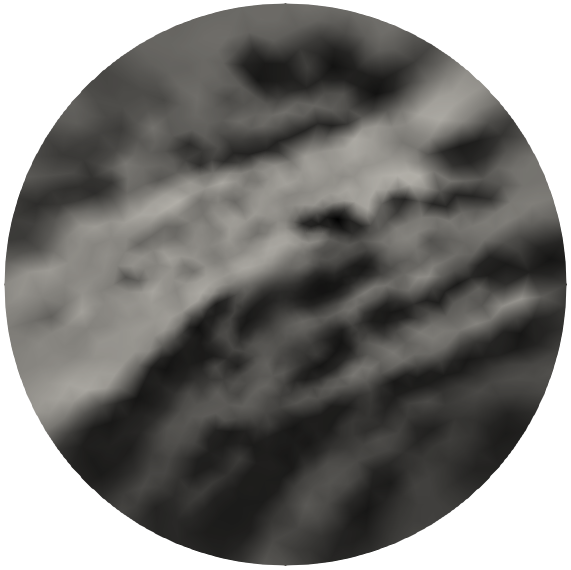
\includegraphics[scale=0.18]{figures/mstar_0.01noise_cropped.png}
  \end{figure}
  \begin{center}
    The log basal sliding parameter computed from the PDE-constrained
    optimization problem with noise levels: $25\%$ (left), $5.0\%$
    (middle), and $1.0\%$ (right).
  \end{center}
\end{frame}
%---------------------------------------------------------------------
\begin{frame}
  \frametitle{Example: Ice sheet inverse problem}
  \framesubtitle{Convergence history for solving the Stokes inverse problem using inexact Newton PCG}

  \only<1>{
  \begin{table}
	{\small
		\begin{center}
			\begingroup
			\setlength{\tabcolsep}{3pt}
			\renewcommand{\arraystretch}{1.1}
			\begin{tabular}{c| c c c | c c c | c c c}
				&  \multicolumn{3}{|c|}{PSF (5)} & \multicolumn{3}{|c|}{REG} & \multicolumn{3}{|c}{NONE} \\
				\hline
				Iter & 
				\#CG & \#Stokes & $\|\mathbf{g}\|$ & 
				\#CG & \#Stokes & $\|\mathbf{g}\|$ & 
				\#CG & \#Stokes & $\|\mathbf{g}\|$ \\
				0 &
				1 & 4 & 1.9e+7 &
				3 & 8 & 1.9e+7 &
				1 & 4 & 1.9e+7 \\
				1 &
				2 & 6  & 6.1e+6 &
				8 & 18 & 8.4e+6 &
				2 & 6  & 6.1e+6 \\
				2 &
				4 & 10 & 2.6e+6 &
				16 & 34 & 4.1e+6 &
				4 & 10 & 2.6e+6 \\
				3 &
				2 & 6+22 & 6.9e+5 &
				34 & 70 & 1.8e+6 &
				14 & 30 & 6.9e+5 \\
				4 &
				3 & 8 & 4.4e+4 &
				52 & 106 & 5.6e+5 &
				29 & 60 & 1.3e+5 \\
				5 &
				5 & 12 & 2.2e+3 &
				79 & 160 & 9.4e+4 &
				38 & 78 & 1.0e+4 \\
				6 &
				0 & 2 & 1.1e+1 &
				102 & 206 & 6.5e+3 &
				58 & 118 & 1.8e+2 \\
				7 &
				--- & --- & --- &
				151 & 304 & 1.2e+2 &
				0 & 2 & 5.5e-1 \\
				8 & 
				--- & --- & --- &
				0 & 2 & 2.9e-1 &
				--- & --- & --- \\
				\hline
				Total & 
				17 & 70 & --- &
				445 & 908 & --- &
				146 & 308 & --- \\
			\end{tabular}
			\endgroup
		\end{center}
	}
\end{table}
  }

  \only<2>{
    \begin{table}
	{\small
		\begin{center}
			\begingroup
			\setlength{\tabcolsep}{3pt}
			\renewcommand{\arraystretch}{1.1}
			\begin{tabular}{c| c c c | c c c | c c c}
				&  \multicolumn{3}{|c|}{PSF (5)} & \multicolumn{3}{|c|}{REG} & \multicolumn{3}{|c}{NONE} \\
				\hline
				Iter & 
				\#CG & \#Stokes & $\|\mathbf{g}\|$ & 
				\#CG & \#Stokes & $\|\mathbf{g}\|$ & 
				\#CG & \#Stokes & $\|\mathbf{g}\|$ \\
				0 &
				1 & 4 & 1.9e+7 &
				3 & 8 & 1.9e+7 &
				1 & 4 & 1.9e+7 \\
				1 &
				2 & 6  & 6.1e+6 &
				8 & 18 & 8.4e+6 &
				2 & 6  & 6.1e+6 \\
				2 &
				4 & 10 & 2.6e+6 &
				16 & 34 & 4.1e+6 &
				4 & 10 & 2.6e+6 \\
				3 &
				2 & 6+22 & 6.9e+5 &
				34 & 70 & 1.8e+6 &
				14 & 30 & 6.9e+5 \\
				4 &
				3 & 8 & 4.4e+4 &
				52 & 106 & 5.6e+5 &
				29 & 60 & 1.3e+5 \\
				5 &
				5 & 12 & 2.2e+3 &
				79 & 160 & 9.4e+4 &
				38 & 78 & 1.0e+4 \\
				6 &
				0 & 2 & 1.1e+1 &
				102 & 206 & 6.5e+3 &
				58 & 118 & 1.8e+2 \\
				7 &
				--- & --- & --- &
				151 & 304 & 1.2e+2 &
				0 & 2 & 5.5e-1 \\
				8 & 
				--- & --- & --- &
				0 & 2 & 2.9e-1 &
				--- & --- & --- \\
				\hline
				Total & 
				17 & {\bf \alert{70}} & --- &
				445 & {\bf \alert{908}} & --- &
				146 & {\bf \alert{308}} & --- \\
			\end{tabular}
			\endgroup
		\end{center}
	}
\end{table}  
  }
  
  \footnotesize
  \begin{itemize}
  \item \#CG:  the number of PCG iterations used to solve the Newton system.
  \item \#Stokes:the total number of Stokes PDE solves performed in each Newton iteration.
  \item $\|\mathbf{g}\|$: the $l^2$ norm of the gradient.
  \end{itemize}
\end{frame}
%---------------------------------------------------------------------
\begin{frame}
  \frametitle{Example: Ice sheet inverse problem}
  \framesubtitle{Convergence history and eigenvalue clustering}

  \begin{figure}
    \begin{center}
    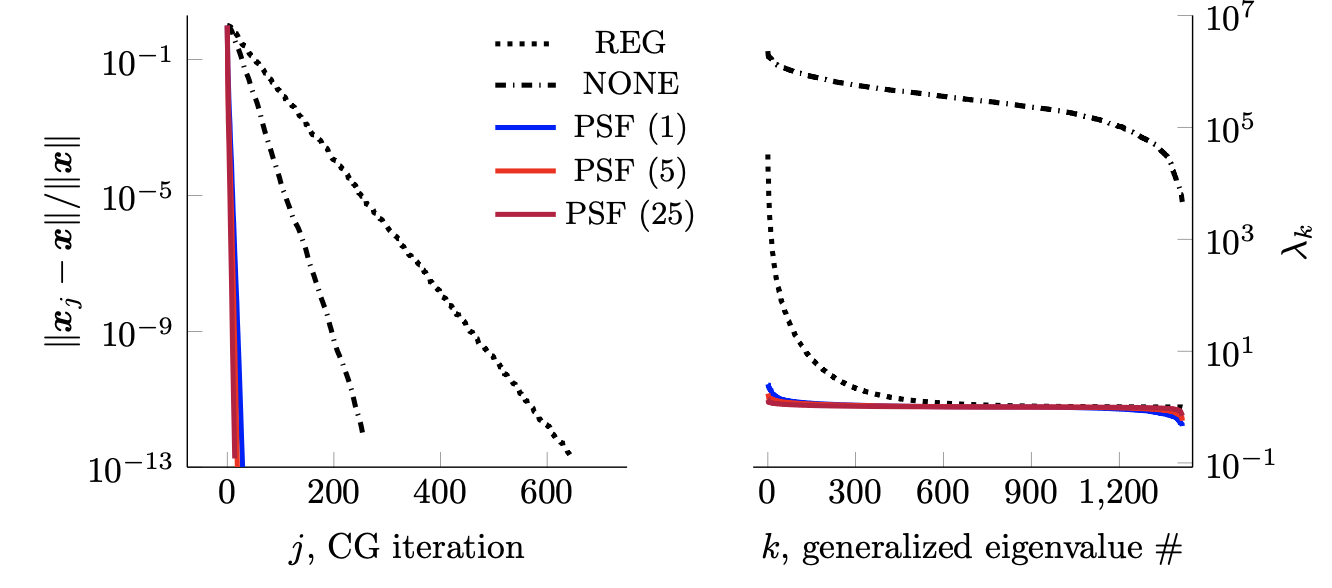
\includegraphics[width=0.85\columnwidth]{extraplots/bbb}
    \end{center}
  \end{figure}
  \begin{center}
    Left: convergence history for solving $\mathbf{H} \mathbf{x} = \mathbf{b}$
    using PCG, where $\mathbf{b}$ has i.i.d. random entries drawn from the
    standard Gaussian distribution and $\mathbf{H}$ is evaluated at the
    solution of the inverse problem. Right: generalized eigenvalues
    for generalized eigenvalue problem $\mathbf{H} \mathbf{u}_{k}=\lambda_{k}
    \mathbf{\preconditioner} \mathbf{u}_{k}$.
  \end{center}
\end{frame}
%---------------------------------------------------------------------
\begin{frame}
  \frametitle{Example: Ice sheet inverse problem}

  \begin{table}
    \begin{center}
      \begingroup
      \setlength{\tabcolsep}{4pt}
      \renewcommand{\arraystretch}{1.25}
      \begin{tabular}{c| c c c c c}
	noise    & \multicolumn{5}{c}{COND$(\mathbf{\preconditioner}^{-1} \mathbf{H})$ } \\ \cline{2-6}
	level    & REG     &	NONE  & PSF $(1)$ & PSF $(5)$ & PSF $(25)$ \\ \hline 
	$25\%$   & 1.01e+3 & 2.96e+3  & 1.34e+0   & 1.30e+0   & 1.18e+0    \\ 
	$11\%$   & 7.40e+3 & 1.05e+3  & 2.27e+0   & 1.55e+0   & 1.31e+0    \\   
	$5.0\%$  & 3.29e+4 & 4.96e+2  & 5.61e+0   & 3.06e+0   & 1.92e+0    \\ 
	$2.2\%$  & 1.66e+5 & 8.89e+2  & 1.58e+1   & 8.07e+0   & 4.03e+0    \\  
	$1.0\%$  & 5.36e+5 & 1.61e+3  & 7.17e+1   & 1.93e+1   & 9.19e+0    \\   
      \end{tabular}
      \endgroup
    \end{center}
  \end{table}

  \begin{center}
  Condition number for $\mathbf{\preconditioner}^{-1} \mathbf{H}$ for
  the PSF-based preconditioners with 1, 5, and 25 batches (PSF (1),
  PSF (5), and PSF(25), respectively), no preconditioner (NONE) and
  regularization (REG).
  \end{center}  
\end{frame}

%------------------------------------------------------------------------------------------------------------
\begin{frame}
  \frametitle{Comparison of cost to approximate the blur kernel}
  
  \begin{table}
    \begin{center}
      {\small
	\begingroup
	\setlength{\tabcolsep}{8pt}
	\renewcommand{\arraystretch}{1.0}
	\begin{tabular}{c| c | c c c c c}
	  & {\bf Error}    &	{\bf \#applies PSF}   & {\bf \#applies HODLR} 	& {\bf \#applies RSVD} 	\\%& rank \\ 
	  \hline 
	  & 20\%    		& 11  				& 592				& 354				\\%& 111  \\ 
	  $L=1$ 		& 10\% 			& 15  				& 772				& 520				\\%& 178  \\ 
	  & 5\% 			& 23   				& 924				& 674				\\%& 244 \\ 
	  \hline
	  & 20\%    		& 8  				& 852 				& 1316				\\%& 417 \\ 
	  $L=1/2$ 	& 10\%    		& 10  				& 1144				& 1916				\\%& 665 \\ 
	  & 5\% 	  		& 12   				& 1404				& 2456				\\%& 903 \\ 
	  \hline
	  & 20\%    	 	& 7					& 932				& 2624				\\%& 845  \\ 
	  $L=1/3$ 	& 10\%    		& 8  				& 1264 				& 3734				\\%& 1321  \\ 
	  & 5\% 			& 8   				& 1520 				& 4660				\\%& 1759  \\ 
	\end{tabular}
	\endgroup
      }
    \end{center}
%\caption{(Spatially variant blur) Comparison of cost to
%  approximate the blur kernel from Equation
%  \eqref{eq:frog_kernel} using the PSF method, the randomized
%  HODLR (hierarchical off diagonal low rank) method, and GLR
%  (global low rank) approximation using randomized SVD. The
%  quantity $L$ scales the width of the impulse responses,
%  hence it influences the rank of the operator. Large $L$
%  means low rank, and small $L$ means high rank. The second
%  column (``Error tol'') is the relative error in the
%  approximation of the kernel measured in the Frobenius norm,
%  $||\Phi - \widetilde{\Phi}||_\text{Fro} /
%  ||\Phi||_\text{Fro}$. The remaining three columns show the
%  number of operator applies required to achieve the given
%  error tolerances, using the PSF, HODLR, and GLR methods.}
%    \label{tab:frog_psf_vs_hodlr_vs_glr}
  \end{table}

  \begin{itemize}
    %\item Comparison of cost to approximate a blur kernel using the
    %  PSF method, the randomized HODLR (hierarchical off diagonal low
    %  rank) method, and GLR (global low rank) approximation using
    %  randomized SVD.
    %\item PSF, HODLR, and GLR
  \item {$L$}: scales the width of the impulse responses (influences the rank)
    %, hence it influences the rank of the operator.
  \item {\bf Error}: is the relative error in the approximation of the
    kernel measured in the Frobenius norm.
  \item {\bf \#applies}: number of operator applies required to achieve
    the given error tolerances, using the {\bf PSF}, {\bf HODLR} (hierarchical
    off diagonal low rank), and {\bf GLR} (global low rank) methods.
  \end{itemize}
  
\end{frame}
 %--------------------------------------------------------------------------
%\begin{frame}
%  \frametitle{Summary and future work}
%
%  \begin{itemize}
%    %\setlength\itemsep{2em}
%  \item Hessian approximations are essential for efficient solution
%    of inverse problems governed by partial differential equations.
%    \vspace{0.05in}
%  \item Low-rank approximations of the Hessian become prohibitive as
%    the data becomes more informative (as is the case for ice sheet
%    inverse problems).
%    \vspace{0.05in}
%  \item Local point spread function interpolation combined with
%    Hierarchical matrix representations yield a highly efficient
%    Hessian approximation.
%
%  \item {\bf Future work:} apply this PSF-based method to the
%    Antarctic ice sheet inverse problem and full Bayesian inversion.
%  \end{itemize}
%
%  \vspace{0.1in}
%  \begin{itemize}
%  \item [] {Details in: N. Alger, T. Hartland, N. Petra,
%    O. Ghattas. ``Point spread function approximation of high rank
%    Hessians with locally supported non-negative integral kernels'',
%    To appear in SIAM Journal on Scientific Computing (SISC).}
%  \end{itemize}
%
%\end{frame}
%--------------------------------------------------------------------------
%\begin{frame}
%  \frametitle{Sessions here at UQ24:}
%  \begin{enumerate}
%    %\setlength\itemsep{2em}
%  \item aaa
%  \end{enumerate}
%
%\end{frame}
%--------------------------------------------------------------------------
\begin{frame}
  \frametitle{The taxonomy of rank-structured matrices}

  \begin{table}
    \begin{center}

      \label{tbl:performance}
      \begin{tabular}{|r|r|r|}
        \hline
        & {\it Weak admissibility}       & {\it Strong admissibility}  \\
        & Simpler data structures. & Lower ranks.\\
        & Good for 1D and 2D.      & Longer interaction lists. \\
        \hline
            {\it General basis matrices:}     & HODLR              & $\Hm$-matrices  \\
            Lower ranks.               &                    & \\
            \hline
                {\it Nested basis matrices:}      & HBS/HSS                & $\Hm^2$-matrices \\
                Enable $O(N)$ complexity.  &                    &\\
                \hline
      \end{tabular}
    \end{center}
  \end{table}

  \vspace{0.1in}
  \small
  \vspace{0.02in}
  \begin{itemize}
  \item HODLR: Hierarchical off-diagonal low-rank matrices
  \item HBS: Hierarchical block separable matrices
  \item HSS: Hierarchically semiseparable matrices

    \vspace{0.05in}
  \item Weak admissibility: all the submatrices except those on the
    diagonal become low-rank.
  \item Strong admissibility: the off-diagonal block is compressed
    only if adjacent blocks are ``well''-separated.
  \end{itemize}

  \vspace{0.1in}
  \scriptsize
  Details in:
  \begin{itemize}
    \scriptsize
  \item [] Per-Gunnar Martinsson, {\it Fast direct solvers for
    elliptic PDEs}, SIAM, 2020.
  \item [] J. Ballani and D. Kressner, {\it Matrices with hierarchical
    low-rank structures, Springer, 2016.}
  \end{itemize}
\end{frame}
%--------------------------------------------------------------------------
\begin{frame}
  \frametitle{References}

  \begin{itemize}
    \setlength\itemsep{2em}
  \item N. Alger, T. Hartland, N. Petra, O. Ghattas. ``Point spread
    function approximation of high rank Hessians with locally
    supported non-negative integral kernels'', To appear in {\bf SIAM
      Journal on Scientific Computing (SISC)}
    (\url{http://arxiv.org/abs/2307.03349}).

    \item T. Hartland, G. Stadler, M. Perego, K. Liegeois,
      N. Petra. ``Hierarchical off-diagonal low-rank approximation of
      Hessians in inverse problems, with application to ice sheet
      model initialization'', {\bf Inverse Problems}, 39 (8), 2023.

    \item T. Isaac, N. Petra, G. Stadler, and O. Ghattas. ``Scalable
      and efficient algorithms for the propagation of uncertainty from
      data through inference to prediction for large-scale problems,
      with application to flow of the Antarctic ice sheet'', {\bf
        Journal of Computational Physics (JCP)}, 296, 348-368 (2015).
  \end{itemize}

\end{frame}
%---------------------------------------------------------------------

\end{document}
